\documentclass[twoside]{book}

% Packages required by doxygen
\usepackage{fixltx2e}
\usepackage{calc}
\usepackage{doxygen}
\usepackage[export]{adjustbox} % also loads graphicx
\usepackage{graphicx}
\usepackage[utf8]{inputenc}
\usepackage{makeidx}
\usepackage{multicol}
\usepackage{multirow}
\PassOptionsToPackage{warn}{textcomp}
\usepackage{textcomp}
\usepackage[nointegrals]{wasysym}
\usepackage[table]{xcolor}

% Font selection
\usepackage[T1]{fontenc}
\usepackage[scaled=.90]{helvet}
\usepackage{courier}
\usepackage{amssymb}
\usepackage{sectsty}
\renewcommand{\familydefault}{\sfdefault}
\allsectionsfont{%
  \fontseries{bc}\selectfont%
  \color{darkgray}%
}
\renewcommand{\DoxyLabelFont}{%
  \fontseries{bc}\selectfont%
  \color{darkgray}%
}
\newcommand{\+}{\discretionary{\mbox{\scriptsize$\hookleftarrow$}}{}{}}

% Page & text layout
\usepackage{geometry}
\geometry{%
  a4paper,%
  top=2.5cm,%
  bottom=2.5cm,%
  left=2.5cm,%
  right=2.5cm%
}
\tolerance=750
\hfuzz=15pt
\hbadness=750
\setlength{\emergencystretch}{15pt}
\setlength{\parindent}{0cm}
\setlength{\parskip}{3ex plus 2ex minus 2ex}
\makeatletter
\renewcommand{\paragraph}{%
  \@startsection{paragraph}{4}{0ex}{-1.0ex}{1.0ex}{%
    \normalfont\normalsize\bfseries\SS@parafont%
  }%
}
\renewcommand{\subparagraph}{%
  \@startsection{subparagraph}{5}{0ex}{-1.0ex}{1.0ex}{%
    \normalfont\normalsize\bfseries\SS@subparafont%
  }%
}
\makeatother

% Headers & footers
\usepackage{fancyhdr}
\pagestyle{fancyplain}
\fancyhead[LE]{\fancyplain{}{\bfseries\thepage}}
\fancyhead[CE]{\fancyplain{}{}}
\fancyhead[RE]{\fancyplain{}{\bfseries\leftmark}}
\fancyhead[LO]{\fancyplain{}{\bfseries\rightmark}}
\fancyhead[CO]{\fancyplain{}{}}
\fancyhead[RO]{\fancyplain{}{\bfseries\thepage}}
\fancyfoot[LE]{\fancyplain{}{}}
\fancyfoot[CE]{\fancyplain{}{}}
\fancyfoot[RE]{\fancyplain{}{\bfseries\scriptsize Generated by Doxygen }}
\fancyfoot[LO]{\fancyplain{}{\bfseries\scriptsize Generated by Doxygen }}
\fancyfoot[CO]{\fancyplain{}{}}
\fancyfoot[RO]{\fancyplain{}{}}
\renewcommand{\footrulewidth}{0.4pt}
\renewcommand{\chaptermark}[1]{%
  \markboth{#1}{}%
}
\renewcommand{\sectionmark}[1]{%
  \markright{\thesection\ #1}%
}

% Indices & bibliography
\usepackage{natbib}
\usepackage[titles]{tocloft}
\setcounter{tocdepth}{3}
\setcounter{secnumdepth}{5}
\makeindex

% Hyperlinks (required, but should be loaded last)
\usepackage{ifpdf}
\ifpdf
  \usepackage[pdftex,pagebackref=true]{hyperref}
\else
  \usepackage[ps2pdf,pagebackref=true]{hyperref}
\fi
\hypersetup{%
  colorlinks=true,%
  linkcolor=blue,%
  citecolor=blue,%
  unicode%
}

% Custom commands
\newcommand{\clearemptydoublepage}{%
  \newpage{\pagestyle{empty}\cleardoublepage}%
}

\usepackage{caption}
\captionsetup{labelsep=space,justification=centering,font={bf},singlelinecheck=off,skip=4pt,position=top}

%===== C O N T E N T S =====

\begin{document}

% Titlepage & ToC
\hypersetup{pageanchor=false,
             bookmarksnumbered=true,
             pdfencoding=unicode
            }
\pagenumbering{roman}
\begin{titlepage}
\vspace*{7cm}
\begin{center}%
{\Large Listen\+To\+Me }\\
\vspace*{1cm}
{\large Generated by Doxygen 1.8.11}\\
\end{center}
\end{titlepage}
\clearemptydoublepage
\tableofcontents
\clearemptydoublepage
\pagenumbering{arabic}
\hypersetup{pageanchor=true}

%--- Begin generated contents ---
\chapter{W\+C\+F-\/\+Service Service1 Dokumentation}
\label{index}\hypertarget{index}{}\hypertarget{index_zero}{}\section{Prerequisites}\label{index_zero}
To run Listen\+App, you need
\begin{DoxyItemize}
\item Visual Studio C\# developing environment
\item Windows 10 dektop with Cortana. Some functionalities might be available in Windows 8.\+1+ as well as in Windows Phone Versions, I\textquotesingle{}m not guaranteeing that however, since it\textquotesingle{}s not tested.
\item to be registered as a user in the webform (the userename and password is needed for most methods, except when running in Mock-\/\+Mode)
\item there are a number of other registrations that the App needs and that I have already provided in the background. If I will ever shut down those online services, you will have to create those on your own as follows\+:
\begin{DoxyEnumerate}
\item Microsoft Developer Account
\item L\+U\+IS Account
\item Azure Account
\item Bot Developer Account
\item Cortana Developer Account -\/microphone permission on your device is preferable. Otherwise you will be only able to run the App in text-\/mode.
\end{DoxyEnumerate}
\end{DoxyItemize}\hypertarget{index_first}{}\section{Functionality}\label{index_first}
Listen\+App is the main component of \mbox{\hyperlink{namespace_listen_to_me}{Listen\+To\+Me}} project. It contains a visual representation of the online form E\+SF and an text or speech input line. Input is evaluated by sending the phrases to the online Service L\+U\+IS or to the online Service Bot with Send\+Message(), and then evaluating the response in dertermine\+Response(). The available, enabled input fields at the App as well as radio buttons and dropdown lists are referenced in a Hashtable with their labels as keys. If the App recognizes a match with one of the labels in the App, it will fill in the recognised field value in the phrase into that very field. If it is not sure -\/ sometimes there are several inputs with the same label -\/ it will ask the user for disambiguation. As it is, Listen\+App can\textquotesingle{}t upload the data back to the online form. There is a in GO written component formularinstanzservice that has to be addressed for that and I haven\textquotesingle{}t yet figured out how to do that.\hypertarget{index_second}{}\section{Pecularities}\label{index_second}
The W\+CF Service is implemented in Factory Pattern. The facory is able to produce either in Mock-\/\+Mode or in Real-\/\+Mode output. Mock-\/\+Mode is independant from the availability of the form to be parsed. It reads from a text file called Sections.\+json which is included in the project. Real-\/\+Mode however, does call the domain of the webform to archieve the same purpose.

If the app is throwing a C\+O\+M\+Exception, the problem is that it can\textquotesingle{}t find the W\+CF Service on which it depends. The workaround for this is to delete the service reference in the app, rebuild the W\+CF Service project and create a new service reference to the Service1.\+svc of W\+CF Service project in this app.\hypertarget{index_third}{}\section{To\+Dos}\label{index_third}

\begin{DoxyItemize}
\item Die Buttons zum Hinzufügen von Tabellenzeilen bei den favorisierten Bildungsanbietern sind nicht ohne weiteres darstellbar. Aufgrund der Tabellenstruktur im H\+T\+M\+L-\/\+Code, die sehr schwer mit X\+P\+A\+TH auslesbar sein wird, sind die Feldbeschriftungen zugeteilt.
\item Testen, ob cut\+Leading\+Numbers in W\+C\+F\+Service tatsächlich die führenden Nummern aus den Feldern Gründungsdatum ect. schneidet. Wichtig für Bot.
\item Der Selenium\+Browser von W\+CF Service wird nicht beendet
\item Das Formular in Polnisch und Englisch abrufen -\/$>$ neue Dummyelemente generieren
\item Der W\+CF Service ist extrem spezifisch auf das vorliegende Formular hörig. Da er als Grundlage die Html-\/\+Seite parst, hat er keinen zugriff auf die Dahinterliegende Logik, zum Beispiel die Angular-\/\+Direktiven, die dafür sorgen, dass in einem bestimmten Feld eine Summe eingetragen wird, sobald ein anderes ausgefüllt ist. Die Darstellung der dynamischen Inhalte kann er nicht abbilden, z.\+B. Berechnungen, wieviele Zeichen noch übrig sind, Fehlermeldungen und Button-\/\+Aktionen.
\item Ressource Binding läuft für die Checkboxes und Radio\+Buttons nicht glatt
\item up\+Load\+To\+Jason() wirft
\end{DoxyItemize}


\begin{DoxyCode}
StatusCode: 400, ReasonPhrase: 'BadArgument', Version: 1.1, Content: System.Net.Http.StreamContent,
       Headers:
\{
  Request-Context: appId=cid-v1:26a3540d-a02a-4998-a060-715488fd769b
  Strict-Transport-Security: max-age=31536000; includeSubDomains; preload
  Request-Id: c60c9469-68e3-40a5-bb8e-beaa61870875
  Cache-Control: no-store, proxy-revalidate, no-cache, max-age=0, private
  Date: Thu, 14 Dec 2017 07:51:09 GMT
  X-Frame-Options: SAMEORIGIN
  X-Powered-By: ASP.NET
  X-Content-Type-Options: nosniff
  Pragma: no-cache
  Apim-Request-Id: c60c9469-68e3-40a5-bb8e-beaa61870875
  Content-Length: 152
  Content-Type: application/json; charset=utf-8
\}
\end{DoxyCode}



\begin{DoxyItemize}
\item das Codesnippet in den Bot einbauen, das die Cortana information zur email und username abruft, möglich?
\item ändere meine $<$\+Seite$>$ läuft nicht für Seiten, die aus mehr als einem Wort bestehen zum Beispiel \char`\"{}Ändere Listen\+To\+Me Registereintragungen\char`\"{} läuft, nicht aber \char`\"{}ändere listentome rggistereintraggunggen\char`\"{} und \char`\"{}Ändere Listen\+To\+Me Sitz des Antragsstellers\char`\"{}
\end{DoxyItemize}

Kann ich nur zuhause/mit Botframework\+Emulator debuggen\+:
\begin{DoxyItemize}
\item die längeren Eingaben funktionieren nicht mehr wenn Cortana auf U\+SA eingestellt ist \char`\"{}\+Ich möchte die Unternehmensangaben im E\+S\+F\+\_\+2 Formular ausfüllen, z.\+B.\char`\"{}
\item dateiupload und helpdialog stürtzen ab 
\end{DoxyItemize}
\chapter{Namespace Index}
\section{Packages}
Here are the packages with brief descriptions (if available)\+:\begin{DoxyCompactList}
\item\contentsline{section}{\hyperlink{namespace_listen_to_me}{Listen\+To\+Me} }{\pageref{namespace_listen_to_me}}{}
\end{DoxyCompactList}

\chapter{Hierarchical Index}
\section{Class Hierarchy}
This inheritance list is sorted roughly, but not completely, alphabetically\+:\begin{DoxyCompactList}
\item \contentsline{section}{Class\+Library.\+model.\+Bot\+Json}{\pageref{class_class_library_1_1model_1_1_bot_json}}{}
\item Dictionary\begin{DoxyCompactList}
\item \contentsline{section}{Class\+Library.\+model.\+Message}{\pageref{class_class_library_1_1model_1_1_message}}{}
\item \contentsline{section}{Class\+Library.\+model.\+Node}{\pageref{class_class_library_1_1model_1_1_node}}{}
\end{DoxyCompactList}
\item \contentsline{section}{Class\+Library.\+model.\+Form}{\pageref{class_class_library_1_1model_1_1_form}}{}
\item I\+Notify\+Property\+Changed\begin{DoxyCompactList}
\item \contentsline{section}{Class\+Library.\+model.\+Element}{\pageref{class_class_library_1_1model_1_1_element}}{}
\end{DoxyCompactList}
\item \contentsline{section}{Class\+Library.\+model.\+Property}{\pageref{class_class_library_1_1model_1_1_property}}{}
\item \contentsline{section}{Class\+Library.\+model.\+Section}{\pageref{class_class_library_1_1model_1_1_section}}{}
\end{DoxyCompactList}

\chapter{Class Index}
\section{Class List}
Here are the classes, structs, unions and interfaces with brief descriptions\+:\begin{DoxyCompactList}
\item\contentsline{section}{\hyperlink{class_listen_to_me_1_1_app}{Listen\+To\+Me.\+App} \\*contains application specific methods for starting the application. Initializations and state-\/related actions are includes. }{\pageref{class_listen_to_me_1_1_app}}{}
\item\contentsline{section}{\hyperlink{class_listen_to_me_1_1_cortana_model_methods}{Listen\+To\+Me.\+Cortana\+Model\+Methods} \\*Contains methods that update the cortana voice command definition file to make it more dynamic. Note\+: This doesn\textquotesingle{}t work as intendet, because phrase lists are only allowing one word entries and the form headings are mostly more than one word long. }{\pageref{class_listen_to_me_1_1_cortana_model_methods}}{}
\item\contentsline{section}{\hyperlink{class_listen_to_me_1_1_common_1_1_date_time_offset_converter}{Listen\+To\+Me.\+Common.\+Date\+Time\+Offset\+Converter} \\*Convert a Date\+Time to a Date\+Time\+Offset for use by a Date\+Picker, and back to allow for two-\/day data-\/binding. }{\pageref{class_listen_to_me_1_1_common_1_1_date_time_offset_converter}}{}
\item\contentsline{section}{\hyperlink{class_listen_to_me_1_1_view_1_1_disambiguate_view}{Listen\+To\+Me.\+View.\+Disambiguate\+View} \\*}{\pageref{class_listen_to_me_1_1_view_1_1_disambiguate_view}}{}
\item\contentsline{section}{\hyperlink{class_listen_to_me_1_1_dynamic_page}{Listen\+To\+Me.\+Dynamic\+Page} \\*This is a page that can be dynamically filled in \hyperlink{class_listen_to_me_1_1_main_page}{Main\+Page}. It is used to display the components that the wcf service finds per section on the form }{\pageref{class_listen_to_me_1_1_dynamic_page}}{}
\item\contentsline{section}{\hyperlink{class_listen_to_me_1_1_model_1_1_entity}{Listen\+To\+Me.\+Model.\+Entity} \\*subclass of Root\+Object. Note\+: these classes were easily pasted in C\# using the visual studio tools for converting J\+S\+ON }{\pageref{class_listen_to_me_1_1_model_1_1_entity}}{}
\item\contentsline{section}{\hyperlink{class_listen_to_me_1_1_model_1_1_form}{Listen\+To\+Me.\+Model.\+Form} \\*able to store Sections of the form. $<$reference$>$Adventure\+Works in U\+WP sample projects at github$<$/reference$>$ /summary$>$ }{\pageref{class_listen_to_me_1_1_model_1_1_form}}{}
\item\contentsline{section}{\hyperlink{interface_listen_to_me_1_1_common_1_1_i_navigation_service}{Listen\+To\+Me.\+Common.\+I\+Navigation\+Service} \\*Navigation service interface, allows a test implementation to be substituted in its place. }{\pageref{interface_listen_to_me_1_1_common_1_1_i_navigation_service}}{}
\item\contentsline{section}{\hyperlink{class_listen_to_me_1_1_model_1_1_intent}{Listen\+To\+Me.\+Model.\+Intent} \\*subclass of Root\+Object. Note\+: these classes were easily pasted in C\# using the visual studio tools for converting J\+S\+ON }{\pageref{class_listen_to_me_1_1_model_1_1_intent}}{}
\item\contentsline{section}{\hyperlink{class_listen_to_me_1_1_model_1_1_listen_to_me_voice_command}{Listen\+To\+Me.\+Model.\+Listen\+To\+Me\+Voice\+Command} \\*class for storing arguments. used by \hyperlink{class_listen_to_me_1_1_app}{App} to bind launch arguments (e.\+g. from Cortana) }{\pageref{class_listen_to_me_1_1_model_1_1_listen_to_me_voice_command}}{}
\item\contentsline{section}{\hyperlink{class_listen_to_me_1_1_common_1_1_load_state_event_args}{Listen\+To\+Me.\+Common.\+Load\+State\+Event\+Args} \\*Class used to hold the event data required when a page attempts to load state. }{\pageref{class_listen_to_me_1_1_common_1_1_load_state_event_args}}{}
\item\contentsline{section}{\hyperlink{class_listen_to_me_1_1_login_page}{Listen\+To\+Me.\+Login\+Page} \\*retrieves and stores login Information in a password vault to\+Do\+: use this for direct\+Line secret as well }{\pageref{class_listen_to_me_1_1_login_page}}{}
\item\contentsline{section}{\hyperlink{class_listen_to_me_1_1_main_page}{Listen\+To\+Me.\+Main\+Page} \\*contains the navigation buttons of the app as well as the speech input field }{\pageref{class_listen_to_me_1_1_main_page}}{}
\item\contentsline{section}{\hyperlink{class_listen_to_me_1_1_common_1_1_navigation_helper}{Listen\+To\+Me.\+Common.\+Navigation\+Helper} \\*aids in navigation between pages. It manages the backstack and integrates Suspension\+Manager to handle process lifetime management and state management when navigating between pages. }{\pageref{class_listen_to_me_1_1_common_1_1_navigation_helper}}{}
\item\contentsline{section}{\hyperlink{class_listen_to_me_1_1_common_1_1_navigation_service}{Listen\+To\+Me.\+Common.\+Navigation\+Service} \\*Navigation system that decouples the \hyperlink{namespace_listen_to_me_1_1_view}{View} \hyperlink{namespace_listen_to_me_1_1_model}{Model} from knowledge of the \hyperlink{namespace_listen_to_me_1_1_view}{View} for navigation purposes. This class can be replaced with a simple mock implementation for test purposes. }{\pageref{class_listen_to_me_1_1_common_1_1_navigation_service}}{}
\item\contentsline{section}{\hyperlink{class_listen_to_me_1_1_model_1_1_proxy}{Listen\+To\+Me.\+Model.\+Proxy} \\*queries L\+U\+I\+Sbot\+Ai with techniques of Collin Blake from \href{https://www.youtube.com/watch?v=ziLkj4PmcCE}{\tt https\+://www.\+youtube.\+com/watch?v=zi\+Lkj4\+Pmc\+CE} }{\pageref{class_listen_to_me_1_1_model_1_1_proxy}}{}
\item\contentsline{section}{\hyperlink{class_listen_to_me_1_1_common_1_1_root_frame_navigation_helper}{Listen\+To\+Me.\+Common.\+Root\+Frame\+Navigation\+Helper} \\*registers for standard mouse and keyboard shortcuts used to go back and forward. There should be only one instance of this class per view, and it should be associated with the root frame. }{\pageref{class_listen_to_me_1_1_common_1_1_root_frame_navigation_helper}}{}
\item\contentsline{section}{\hyperlink{class_listen_to_me_1_1_model_1_1_rootobject}{Listen\+To\+Me.\+Model.\+Rootobject} \\*models the default L\+U\+IS Http-\/answer which consiscts in a json object providing propabilities of intens together with entity model }{\pageref{class_listen_to_me_1_1_model_1_1_rootobject}}{}
\item\contentsline{section}{\hyperlink{class_listen_to_me_1_1_common_1_1_save_state_event_args}{Listen\+To\+Me.\+Common.\+Save\+State\+Event\+Args} \\*Class used to hold the event data required when a page attempts to save state. }{\pageref{class_listen_to_me_1_1_common_1_1_save_state_event_args}}{}
\item\contentsline{section}{\hyperlink{class_listen_to_me_1_1_view_1_1_section_details}{Listen\+To\+Me.\+View.\+Section\+Details} \\*Code Behind for a list of Sections, including a Save and Delete button. Associated with the Section\+View\+Model for most behaviors and properties. }{\pageref{class_listen_to_me_1_1_view_1_1_section_details}}{}
\item\contentsline{section}{\hyperlink{class_listen_to_me_1_1_view_1_1_section_list_view}{Listen\+To\+Me.\+View.\+Section\+List\+View} \\*Code Behind for a list of Sections, including an Add button. Associated with the Section\+List\+View\+Model for most behaviors and properties. }{\pageref{class_listen_to_me_1_1_view_1_1_section_list_view}}{}
\item\contentsline{section}{\hyperlink{class_listen_to_me_1_1_view_model_1_1_section_list_view_model}{Listen\+To\+Me.\+View\+Model.\+Section\+List\+View\+Model} \\*\hyperlink{namespace_listen_to_me_1_1_view}{View} \hyperlink{namespace_listen_to_me_1_1_model}{Model} controlling the behavior of a List view of Sections }{\pageref{class_listen_to_me_1_1_view_model_1_1_section_list_view_model}}{}
\item\contentsline{section}{\hyperlink{class_listen_to_me_1_1_view_model_1_1_section_view_model}{Listen\+To\+Me.\+View\+Model.\+Section\+View\+Model} \\*\hyperlink{namespace_listen_to_me_1_1_view}{View} \hyperlink{namespace_listen_to_me_1_1_model}{Model} associated with Section\+Details.\+xaml. Provides access to an individual Section, and Commands for saving new, updating existing, and deleting Sections. Is able to both create brand new Sections, and edit existing Sections, hiding buttons that should not be accessible in some cases. }{\pageref{class_listen_to_me_1_1_view_model_1_1_section_view_model}}{}
\item\contentsline{section}{\hyperlink{class_listen_to_me_1_1_common_1_1_suspension_manager_exception}{Listen\+To\+Me.\+Common.\+Suspension\+Manager\+Exception} \\*occurs when the Suspension\+Manager fails e.\+g. at storing the session state of a frame }{\pageref{class_listen_to_me_1_1_common_1_1_suspension_manager_exception}}{}
\item\contentsline{section}{\hyperlink{class_listen_to_me_1_1_model_1_1_topscoringintent}{Listen\+To\+Me.\+Model.\+Topscoringintent} \\*subclass of Root\+Object. Note\+: these classes were easily pasted in C\# using the visual studio tools for converting J\+S\+ON }{\pageref{class_listen_to_me_1_1_model_1_1_topscoringintent}}{}
\item\contentsline{section}{\hyperlink{class_listen_to_me_1_1_view_model_1_1_view_model_base}{Listen\+To\+Me.\+View\+Model.\+View\+Model\+Base} \\*Base class for all view models. Contains the common implementation of I\+Notify\+Property\+Changed and the notification helper method. }{\pageref{class_listen_to_me_1_1_view_model_1_1_view_model_base}}{}
\item\contentsline{section}{\hyperlink{class_listen_to_me_1_1_view_model_1_1_view_model_locator}{Listen\+To\+Me.\+View\+Model.\+View\+Model\+Locator} \\*\hyperlink{class_listen_to_me_1_1_view_model_1_1_view_model_locator}{View\+Model\+Locator} ensures that viewmodels can be instantiated with a common reference to the Section\+Store. This allows for easier decoupling of the store implementation and the view models, and allows for less viewmodel specific code in the views. }{\pageref{class_listen_to_me_1_1_view_model_1_1_view_model_locator}}{}
\end{DoxyCompactList}

\chapter{File Index}
\section{File List}
Here is a list of all files with brief descriptions\+:\begin{DoxyCompactList}
\item\contentsline{section}{C\+:/\+Users/user/source/repos/\+Hoermirzu/\+Listen\+To\+Me-\/master-\/89f0b49594deaade7bfad24dad062ff16eca36da/\+Listen\+To\+Me/\hyperlink{_app_8xaml_8cs}{App.\+xaml.\+cs} }{\pageref{_app_8xaml_8cs}}{}
\item\contentsline{section}{C\+:/\+Users/user/source/repos/\+Hoermirzu/\+Listen\+To\+Me-\/master-\/89f0b49594deaade7bfad24dad062ff16eca36da/\+Listen\+To\+Me/\hyperlink{_bot_8cs}{Bot.\+cs} }{\pageref{_bot_8cs}}{}
\item\contentsline{section}{C\+:/\+Users/user/source/repos/\+Hoermirzu/\+Listen\+To\+Me-\/master-\/89f0b49594deaade7bfad24dad062ff16eca36da/\+Listen\+To\+Me/\hyperlink{_content_page_8cs}{Content\+Page.\+cs} }{\pageref{_content_page_8cs}}{}
\item\contentsline{section}{C\+:/\+Users/user/source/repos/\+Hoermirzu/\+Listen\+To\+Me-\/master-\/89f0b49594deaade7bfad24dad062ff16eca36da/\+Listen\+To\+Me/\hyperlink{_cortana_model_methods_8cs}{Cortana\+Model\+Methods.\+cs} }{\pageref{_cortana_model_methods_8cs}}{}
\item\contentsline{section}{C\+:/\+Users/user/source/repos/\+Hoermirzu/\+Listen\+To\+Me-\/master-\/89f0b49594deaade7bfad24dad062ff16eca36da/\+Listen\+To\+Me/\hyperlink{_dynamic_page_8xaml_8cs}{Dynamic\+Page.\+xaml.\+cs} }{\pageref{_dynamic_page_8xaml_8cs}}{}
\item\contentsline{section}{C\+:/\+Users/user/source/repos/\+Hoermirzu/\+Listen\+To\+Me-\/master-\/89f0b49594deaade7bfad24dad062ff16eca36da/\+Listen\+To\+Me/\hyperlink{_i_model_methods_8cs}{I\+Model\+Methods.\+cs} }{\pageref{_i_model_methods_8cs}}{}
\item\contentsline{section}{C\+:/\+Users/user/source/repos/\+Hoermirzu/\+Listen\+To\+Me-\/master-\/89f0b49594deaade7bfad24dad062ff16eca36da/\+Listen\+To\+Me/\hyperlink{_login_page_8xaml_8cs}{Login\+Page.\+xaml.\+cs} }{\pageref{_login_page_8xaml_8cs}}{}
\item\contentsline{section}{C\+:/\+Users/user/source/repos/\+Hoermirzu/\+Listen\+To\+Me-\/master-\/89f0b49594deaade7bfad24dad062ff16eca36da/\+Listen\+To\+Me/\hyperlink{_main_page_8xaml_8cs}{Main\+Page.\+xaml.\+cs} }{\pageref{_main_page_8xaml_8cs}}{}
\end{DoxyCompactList}

\chapter{Namespace Documentation}
\hypertarget{namespace_wcf_service1}{}\section{Wcf\+Service1 Namespace Reference}
\label{namespace_wcf_service1}\index{Wcf\+Service1@{Wcf\+Service1}}
\subsection*{Classes}
\begin{DoxyCompactItemize}
\item 
class \hyperlink{class_wcf_service1_1_1_alexa}{Alexa}
\begin{DoxyCompactList}\small\item\em provides code for connecting to an \hyperlink{class_wcf_service1_1_1_alexa}{Alexa} skill. Not tested. reference\+: \href{https://www.robinosborne.co.uk/2016/12/19/connecting-alexa-to-a-botframework-chatbot/}{\tt https\+://www.\+robinosborne.\+co.\+uk/2016/12/19/connecting-\/alexa-\/to-\/a-\/botframework-\/chatbot/} \end{DoxyCompactList}\item 
class \hyperlink{class_wcf_service1_1_1_cortana_direct_line_client}{Cortana\+Direct\+Line\+Client}
\begin{DoxyCompactList}\small\item\em creates Direct\+Line connection to the bot \end{DoxyCompactList}\item 
class \hyperlink{class_wcf_service1_1_1_implementation___mock}{Implementation\+\_\+\+Mock}
\item 
class \hyperlink{class_wcf_service1_1_1_implementation___real}{Implementation\+\_\+\+Real}
\item 
class \hyperlink{class_wcf_service1_1_1_implementation_factory}{Implementation\+Factory}
\begin{DoxyCompactList}\small\item\em reference\+: \href{http://www.c-sharpcorner.com/article/factory-method-design-pattern-in-c-sharp/}{\tt http\+://www.\+c-\/sharpcorner.\+com/article/factory-\/method-\/design-\/pattern-\/in-\/c-\/sharp/} \end{DoxyCompactList}\item 
interface \hyperlink{interface_wcf_service1_1_1_i_service1}{I\+Service1}
\item 
class \hyperlink{class_wcf_service1_1_1_service1}{Service1}
\begin{DoxyCompactList}\small\item\em the class implements the webservice parsing the form. ther is a debug and no-\/debug mode. If Debug is true, the form is build from a json text fine. If not it\textquotesingle{}s delivered fróm a Selenium Browser \hyperlink{class_wcf_service1_1_1_website_crawler}{Website\+Crawler} \end{DoxyCompactList}\item 
class \hyperlink{class_wcf_service1_1_1_service1_factory}{Service1\+Factory}
\item 
class \hyperlink{class_wcf_service1_1_1_service_class}{Service\+Class}
\begin{DoxyCompactList}\small\item\em contains operations of the service1client for parsing the html-\/webform All operations containing a \char`\"{}1\char`\"{} are Dummy-\/\+Operations that only run on files simulating the webform \end{DoxyCompactList}\item 
class \hyperlink{class_wcf_service1_1_1_website_crawler}{Website\+Crawler}
\begin{DoxyCompactList}\small\item\em this class is opening a connection to the web form. I provides methods for retreiving the H\+T\+M\+L-\/\+Code behind a spechific form. \end{DoxyCompactList}\end{DoxyCompactItemize}

\chapter{Class Documentation}
\hypertarget{class_wcf_service1_1_1_alexa}{}\section{Wcf\+Service1.\+Alexa Class Reference}
\label{class_wcf_service1_1_1_alexa}\index{Wcf\+Service1.\+Alexa@{Wcf\+Service1.\+Alexa}}


provides code for connecting to an \hyperlink{class_wcf_service1_1_1_alexa}{Alexa} skill. Not tested. reference\+: \href{https://www.robinosborne.co.uk/2016/12/19/connecting-alexa-to-a-botframework-chatbot/}{\tt https\+://www.\+robinosborne.\+co.\+uk/2016/12/19/connecting-\/alexa-\/to-\/a-\/botframework-\/chatbot/}  




Inheritance diagram for Wcf\+Service1.\+Alexa\+:\nopagebreak
\begin{figure}[H]
\begin{center}
\leavevmode
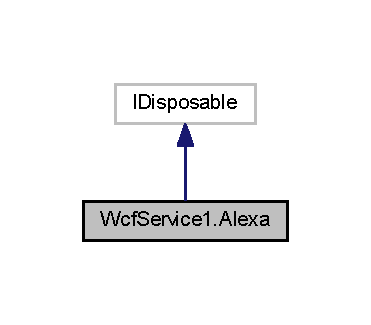
\includegraphics[width=178pt]{class_wcf_service1_1_1_alexa__inherit__graph}
\end{center}
\end{figure}


Collaboration diagram for Wcf\+Service1.\+Alexa\+:\nopagebreak
\begin{figure}[H]
\begin{center}
\leavevmode
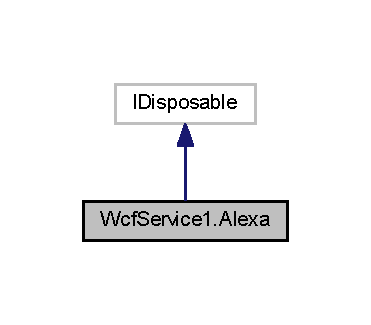
\includegraphics[width=178pt]{class_wcf_service1_1_1_alexa__coll__graph}
\end{center}
\end{figure}
\subsection*{Public Member Functions}
\begin{DoxyCompactItemize}
\item 
\hyperlink{class_wcf_service1_1_1_alexa_a4d589d523e0b283f94c1e2507ef4700f}{Alexa} (string secret, string from)
\item 
async Task$<$ I\+Enumerable$<$ string $>$ $>$ \hyperlink{class_wcf_service1_1_1_alexa_a6222dd6b2c2bc8da8ece2321ad2090ed}{Fetch\+Recent\+Replies} ()
\item 
async Task \hyperlink{class_wcf_service1_1_1_alexa_a6d8d3cc497642584fa380f1cbf053f66}{Send\+Message} (string outgoing\+Text)
\item 
void \hyperlink{class_wcf_service1_1_1_alexa_a7dfa3adcc0c14cf1863daafac2ff5c37}{Dispose} ()
\end{DoxyCompactItemize}
\subsection*{Public Attributes}
\begin{DoxyCompactItemize}
\item 
Http\+Client \hyperlink{class_wcf_service1_1_1_alexa_a62b57286b8d06d2328d1c160bd80f7c5}{Client}
\end{DoxyCompactItemize}
\subsection*{Private Member Functions}
\begin{DoxyCompactItemize}
\item 
async Task$<$ Http\+Client $>$ \hyperlink{class_wcf_service1_1_1_alexa_a2e9aee5a18c8690845046d1da09e60b2}{Create\+Http\+Client} ()
\end{DoxyCompactItemize}
\subsection*{Private Attributes}
\begin{DoxyCompactItemize}
\item 
string \hyperlink{class_wcf_service1_1_1_alexa_abe74124f288adbe9661da5a83ae0051c}{\+\_\+conversation\+Id}
\item 
readonly string \hyperlink{class_wcf_service1_1_1_alexa_a1c94ae34da8665a0918b04cbdfe7707e}{\+\_\+from}
\item 
readonly string \hyperlink{class_wcf_service1_1_1_alexa_a7619c280d871d3abd9db45e733ffaaa5}{\+\_\+secret}
\item 
string \hyperlink{class_wcf_service1_1_1_alexa_a7c8ee921966bce4aa52953d9a148e69b}{Messages\+Path} =$>$ \$\char`\"{}/api/conversations/\{\hyperlink{class_wcf_service1_1_1_alexa_abe74124f288adbe9661da5a83ae0051c}{\+\_\+conversation\+Id}\}/messages\char`\"{}
\end{DoxyCompactItemize}


\subsection{Detailed Description}
provides code for connecting to an \hyperlink{class_wcf_service1_1_1_alexa}{Alexa} skill. Not tested. reference\+: \href{https://www.robinosborne.co.uk/2016/12/19/connecting-alexa-to-a-botframework-chatbot/}{\tt https\+://www.\+robinosborne.\+co.\+uk/2016/12/19/connecting-\/alexa-\/to-\/a-\/botframework-\/chatbot/} 



\subsection{Constructor \& Destructor Documentation}
\index{Wcf\+Service1\+::\+Alexa@{Wcf\+Service1\+::\+Alexa}!Alexa@{Alexa}}
\index{Alexa@{Alexa}!Wcf\+Service1\+::\+Alexa@{Wcf\+Service1\+::\+Alexa}}
\subsubsection[{\texorpdfstring{Alexa(string secret, string from)}{Alexa(string secret, string from)}}]{\setlength{\rightskip}{0pt plus 5cm}Wcf\+Service1.\+Alexa.\+Alexa (
\begin{DoxyParamCaption}
\item[{string}]{secret, }
\item[{string}]{from}
\end{DoxyParamCaption}
)}\hypertarget{class_wcf_service1_1_1_alexa_a4d589d523e0b283f94c1e2507ef4700f}{}\label{class_wcf_service1_1_1_alexa_a4d589d523e0b283f94c1e2507ef4700f}


Here is the call graph for this function\+:\nopagebreak
\begin{figure}[H]
\begin{center}
\leavevmode
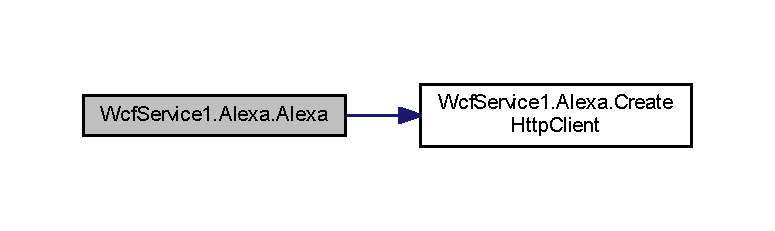
\includegraphics[width=350pt]{class_wcf_service1_1_1_alexa_a4d589d523e0b283f94c1e2507ef4700f_cgraph}
\end{center}
\end{figure}




\subsection{Member Function Documentation}
\index{Wcf\+Service1\+::\+Alexa@{Wcf\+Service1\+::\+Alexa}!Create\+Http\+Client@{Create\+Http\+Client}}
\index{Create\+Http\+Client@{Create\+Http\+Client}!Wcf\+Service1\+::\+Alexa@{Wcf\+Service1\+::\+Alexa}}
\subsubsection[{\texorpdfstring{Create\+Http\+Client()}{CreateHttpClient()}}]{\setlength{\rightskip}{0pt plus 5cm}async Task$<$Http\+Client$>$ Wcf\+Service1.\+Alexa.\+Create\+Http\+Client (
\begin{DoxyParamCaption}
{}
\end{DoxyParamCaption}
)\hspace{0.3cm}{\ttfamily [private]}}\hypertarget{class_wcf_service1_1_1_alexa_a2e9aee5a18c8690845046d1da09e60b2}{}\label{class_wcf_service1_1_1_alexa_a2e9aee5a18c8690845046d1da09e60b2}


Here is the caller graph for this function\+:\nopagebreak
\begin{figure}[H]
\begin{center}
\leavevmode
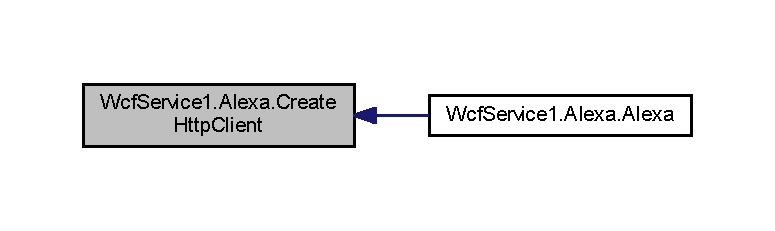
\includegraphics[width=350pt]{class_wcf_service1_1_1_alexa_a2e9aee5a18c8690845046d1da09e60b2_icgraph}
\end{center}
\end{figure}


\index{Wcf\+Service1\+::\+Alexa@{Wcf\+Service1\+::\+Alexa}!Dispose@{Dispose}}
\index{Dispose@{Dispose}!Wcf\+Service1\+::\+Alexa@{Wcf\+Service1\+::\+Alexa}}
\subsubsection[{\texorpdfstring{Dispose()}{Dispose()}}]{\setlength{\rightskip}{0pt plus 5cm}void Wcf\+Service1.\+Alexa.\+Dispose (
\begin{DoxyParamCaption}
{}
\end{DoxyParamCaption}
)}\hypertarget{class_wcf_service1_1_1_alexa_a7dfa3adcc0c14cf1863daafac2ff5c37}{}\label{class_wcf_service1_1_1_alexa_a7dfa3adcc0c14cf1863daafac2ff5c37}
\index{Wcf\+Service1\+::\+Alexa@{Wcf\+Service1\+::\+Alexa}!Fetch\+Recent\+Replies@{Fetch\+Recent\+Replies}}
\index{Fetch\+Recent\+Replies@{Fetch\+Recent\+Replies}!Wcf\+Service1\+::\+Alexa@{Wcf\+Service1\+::\+Alexa}}
\subsubsection[{\texorpdfstring{Fetch\+Recent\+Replies()}{FetchRecentReplies()}}]{\setlength{\rightskip}{0pt plus 5cm}async Task$<$I\+Enumerable$<$string$>$ $>$ Wcf\+Service1.\+Alexa.\+Fetch\+Recent\+Replies (
\begin{DoxyParamCaption}
{}
\end{DoxyParamCaption}
)}\hypertarget{class_wcf_service1_1_1_alexa_a6222dd6b2c2bc8da8ece2321ad2090ed}{}\label{class_wcf_service1_1_1_alexa_a6222dd6b2c2bc8da8ece2321ad2090ed}
\index{Wcf\+Service1\+::\+Alexa@{Wcf\+Service1\+::\+Alexa}!Send\+Message@{Send\+Message}}
\index{Send\+Message@{Send\+Message}!Wcf\+Service1\+::\+Alexa@{Wcf\+Service1\+::\+Alexa}}
\subsubsection[{\texorpdfstring{Send\+Message(string outgoing\+Text)}{SendMessage(string outgoingText)}}]{\setlength{\rightskip}{0pt plus 5cm}async Task Wcf\+Service1.\+Alexa.\+Send\+Message (
\begin{DoxyParamCaption}
\item[{string}]{outgoing\+Text}
\end{DoxyParamCaption}
)}\hypertarget{class_wcf_service1_1_1_alexa_a6d8d3cc497642584fa380f1cbf053f66}{}\label{class_wcf_service1_1_1_alexa_a6d8d3cc497642584fa380f1cbf053f66}


\subsection{Member Data Documentation}
\index{Wcf\+Service1\+::\+Alexa@{Wcf\+Service1\+::\+Alexa}!\+\_\+conversation\+Id@{\+\_\+conversation\+Id}}
\index{\+\_\+conversation\+Id@{\+\_\+conversation\+Id}!Wcf\+Service1\+::\+Alexa@{Wcf\+Service1\+::\+Alexa}}
\subsubsection[{\texorpdfstring{\+\_\+conversation\+Id}{_conversationId}}]{\setlength{\rightskip}{0pt plus 5cm}string Wcf\+Service1.\+Alexa.\+\_\+conversation\+Id\hspace{0.3cm}{\ttfamily [private]}}\hypertarget{class_wcf_service1_1_1_alexa_abe74124f288adbe9661da5a83ae0051c}{}\label{class_wcf_service1_1_1_alexa_abe74124f288adbe9661da5a83ae0051c}
\index{Wcf\+Service1\+::\+Alexa@{Wcf\+Service1\+::\+Alexa}!\+\_\+from@{\+\_\+from}}
\index{\+\_\+from@{\+\_\+from}!Wcf\+Service1\+::\+Alexa@{Wcf\+Service1\+::\+Alexa}}
\subsubsection[{\texorpdfstring{\+\_\+from}{_from}}]{\setlength{\rightskip}{0pt plus 5cm}readonly string Wcf\+Service1.\+Alexa.\+\_\+from\hspace{0.3cm}{\ttfamily [private]}}\hypertarget{class_wcf_service1_1_1_alexa_a1c94ae34da8665a0918b04cbdfe7707e}{}\label{class_wcf_service1_1_1_alexa_a1c94ae34da8665a0918b04cbdfe7707e}
\index{Wcf\+Service1\+::\+Alexa@{Wcf\+Service1\+::\+Alexa}!\+\_\+secret@{\+\_\+secret}}
\index{\+\_\+secret@{\+\_\+secret}!Wcf\+Service1\+::\+Alexa@{Wcf\+Service1\+::\+Alexa}}
\subsubsection[{\texorpdfstring{\+\_\+secret}{_secret}}]{\setlength{\rightskip}{0pt plus 5cm}readonly string Wcf\+Service1.\+Alexa.\+\_\+secret\hspace{0.3cm}{\ttfamily [private]}}\hypertarget{class_wcf_service1_1_1_alexa_a7619c280d871d3abd9db45e733ffaaa5}{}\label{class_wcf_service1_1_1_alexa_a7619c280d871d3abd9db45e733ffaaa5}
\index{Wcf\+Service1\+::\+Alexa@{Wcf\+Service1\+::\+Alexa}!Client@{Client}}
\index{Client@{Client}!Wcf\+Service1\+::\+Alexa@{Wcf\+Service1\+::\+Alexa}}
\subsubsection[{\texorpdfstring{Client}{Client}}]{\setlength{\rightskip}{0pt plus 5cm}Http\+Client Wcf\+Service1.\+Alexa.\+Client}\hypertarget{class_wcf_service1_1_1_alexa_a62b57286b8d06d2328d1c160bd80f7c5}{}\label{class_wcf_service1_1_1_alexa_a62b57286b8d06d2328d1c160bd80f7c5}
\index{Wcf\+Service1\+::\+Alexa@{Wcf\+Service1\+::\+Alexa}!Messages\+Path@{Messages\+Path}}
\index{Messages\+Path@{Messages\+Path}!Wcf\+Service1\+::\+Alexa@{Wcf\+Service1\+::\+Alexa}}
\subsubsection[{\texorpdfstring{Messages\+Path}{MessagesPath}}]{\setlength{\rightskip}{0pt plus 5cm}string Wcf\+Service1.\+Alexa.\+Messages\+Path =$>$ \$\char`\"{}/api/conversations/\{{\bf \+\_\+conversation\+Id}\}/messages\char`\"{}\hspace{0.3cm}{\ttfamily [private]}}\hypertarget{class_wcf_service1_1_1_alexa_a7c8ee921966bce4aa52953d9a148e69b}{}\label{class_wcf_service1_1_1_alexa_a7c8ee921966bce4aa52953d9a148e69b}


The documentation for this class was generated from the following file\+:\begin{DoxyCompactItemize}
\item 
C\+:/\+Users/user/source/repos/\+Hoermirzu/\+Listen\+To\+Me-\/master-\/89f0b49594deaade7bfad24dad062ff16eca36da/\+Wcf\+Service1/\hyperlink{_alexa_8cs}{Alexa.\+cs}\end{DoxyCompactItemize}

\hypertarget{class_wcf_service1_1_1_cortana_direct_line_client}{}\section{Wcf\+Service1.\+Cortana\+Direct\+Line\+Client Class Reference}
\label{class_wcf_service1_1_1_cortana_direct_line_client}\index{Wcf\+Service1.\+Cortana\+Direct\+Line\+Client@{Wcf\+Service1.\+Cortana\+Direct\+Line\+Client}}


creates Direct\+Line connection to the bot  


\subsection*{Public Member Functions}
\begin{DoxyCompactItemize}
\item 
async Task \hyperlink{class_wcf_service1_1_1_cortana_direct_line_client_a71a4d8cff19707b3f6cb0c559b8104f7}{Connect\+Async} ()
\begin{DoxyCompactList}\small\item\em opens a Direct\+Line channel to the bot \end{DoxyCompactList}\item 
async Task$<$ string $>$ \hyperlink{class_wcf_service1_1_1_cortana_direct_line_client_ad9aee7d49dab0e3bb8806349b68716b3}{Talk\+To\+The\+Bot\+Async} (string message)
\begin{DoxyCompactList}\small\item\em sends a message to the bot and retrieves da response for it \end{DoxyCompactList}\end{DoxyCompactItemize}
\subsection*{Private Member Functions}
\begin{DoxyCompactItemize}
\item 
async Task$<$ string $>$ \hyperlink{class_wcf_service1_1_1_cortana_direct_line_client_a0bc2576ae50d7eafd2092bb9cf7e6f7c}{Get\+Response} ()
\begin{DoxyCompactList}\small\item\em retrieves a response from the bot \end{DoxyCompactList}\end{DoxyCompactItemize}
\subsection*{Private Attributes}
\begin{DoxyCompactItemize}
\item 
Direct\+Line\+Client \hyperlink{class_wcf_service1_1_1_cortana_direct_line_client_a2161a12a94efe732c80a2f31f7a91d8d}{\+\_\+direct\+Line}
\begin{DoxyCompactList}\small\item\em client \end{DoxyCompactList}\item 
string \hyperlink{class_wcf_service1_1_1_cortana_direct_line_client_a460c7a68d595773d131142651fa2b213}{\+\_\+conversation\+Id}
\begin{DoxyCompactList}\small\item\em client\textquotesingle{}s conversation id \end{DoxyCompactList}\item 
string \hyperlink{class_wcf_service1_1_1_cortana_direct_line_client_a06b449cbb20e2a97dc873b306371b577}{\+\_\+direct\+Line\+Secret} = Configuration\+Manager.\+App\+Settings\mbox{[}\char`\"{}Direct\+Line\+Secret\char`\"{}\mbox{]}
\begin{DoxyCompactList}\small\item\em the key to the bot\textquotesingle{}s Direct\+Line channel \end{DoxyCompactList}\item 
string \hyperlink{class_wcf_service1_1_1_cortana_direct_line_client_a92b26da0f83e644653c3cd4f8c248b1b}{bot\+Id} = Configuration\+Manager.\+App\+Settings\mbox{[}\char`\"{}Bot\+Id\char`\"{}\mbox{]}
\begin{DoxyCompactList}\small\item\em the bot\textquotesingle{}s microsoft id \end{DoxyCompactList}\item 
readonly string \hyperlink{class_wcf_service1_1_1_cortana_direct_line_client_a5c02c54f3f2ed0d5c508092e516cb5d9}{username} = Configuration\+Manager.\+App\+Settings\mbox{[}\char`\"{}user\+Name\char`\"{}\mbox{]}
\end{DoxyCompactItemize}


\subsection{Detailed Description}
creates Direct\+Line connection to the bot 



\subsection{Member Function Documentation}
\index{Wcf\+Service1\+::\+Cortana\+Direct\+Line\+Client@{Wcf\+Service1\+::\+Cortana\+Direct\+Line\+Client}!Connect\+Async@{Connect\+Async}}
\index{Connect\+Async@{Connect\+Async}!Wcf\+Service1\+::\+Cortana\+Direct\+Line\+Client@{Wcf\+Service1\+::\+Cortana\+Direct\+Line\+Client}}
\subsubsection[{\texorpdfstring{Connect\+Async()}{ConnectAsync()}}]{\setlength{\rightskip}{0pt plus 5cm}async Task Wcf\+Service1.\+Cortana\+Direct\+Line\+Client.\+Connect\+Async (
\begin{DoxyParamCaption}
{}
\end{DoxyParamCaption}
)}\hypertarget{class_wcf_service1_1_1_cortana_direct_line_client_a71a4d8cff19707b3f6cb0c559b8104f7}{}\label{class_wcf_service1_1_1_cortana_direct_line_client_a71a4d8cff19707b3f6cb0c559b8104f7}


opens a Direct\+Line channel to the bot 

\begin{DoxyReturn}{Returns}

\end{DoxyReturn}


Here is the caller graph for this function\+:\nopagebreak
\begin{figure}[H]
\begin{center}
\leavevmode
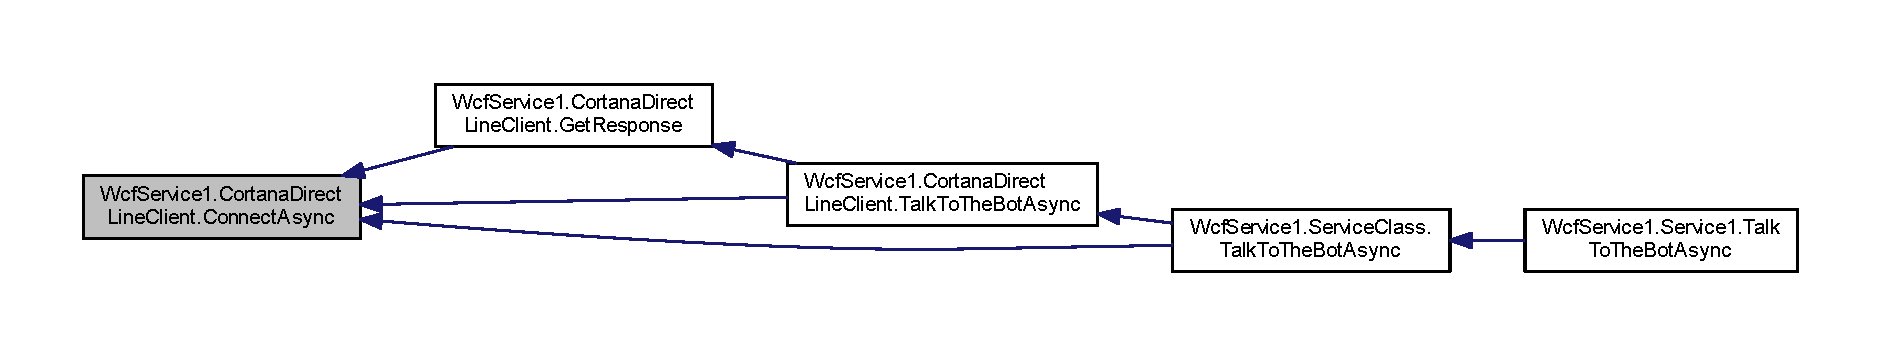
\includegraphics[width=350pt]{class_wcf_service1_1_1_cortana_direct_line_client_a71a4d8cff19707b3f6cb0c559b8104f7_icgraph}
\end{center}
\end{figure}


\index{Wcf\+Service1\+::\+Cortana\+Direct\+Line\+Client@{Wcf\+Service1\+::\+Cortana\+Direct\+Line\+Client}!Get\+Response@{Get\+Response}}
\index{Get\+Response@{Get\+Response}!Wcf\+Service1\+::\+Cortana\+Direct\+Line\+Client@{Wcf\+Service1\+::\+Cortana\+Direct\+Line\+Client}}
\subsubsection[{\texorpdfstring{Get\+Response()}{GetResponse()}}]{\setlength{\rightskip}{0pt plus 5cm}async Task$<$string$>$ Wcf\+Service1.\+Cortana\+Direct\+Line\+Client.\+Get\+Response (
\begin{DoxyParamCaption}
{}
\end{DoxyParamCaption}
)\hspace{0.3cm}{\ttfamily [private]}}\hypertarget{class_wcf_service1_1_1_cortana_direct_line_client_a0bc2576ae50d7eafd2092bb9cf7e6f7c}{}\label{class_wcf_service1_1_1_cortana_direct_line_client_a0bc2576ae50d7eafd2092bb9cf7e6f7c}


retrieves a response from the bot 

\begin{DoxyReturn}{Returns}

\end{DoxyReturn}


Here is the call graph for this function\+:\nopagebreak
\begin{figure}[H]
\begin{center}
\leavevmode
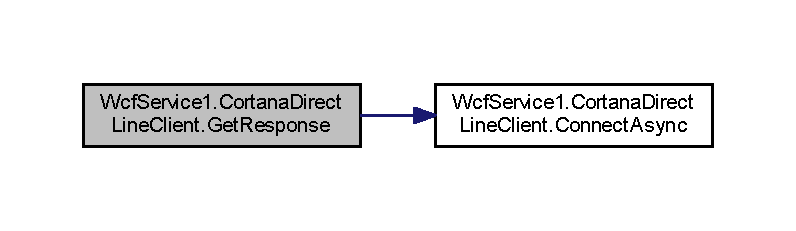
\includegraphics[width=350pt]{class_wcf_service1_1_1_cortana_direct_line_client_a0bc2576ae50d7eafd2092bb9cf7e6f7c_cgraph}
\end{center}
\end{figure}




Here is the caller graph for this function\+:\nopagebreak
\begin{figure}[H]
\begin{center}
\leavevmode
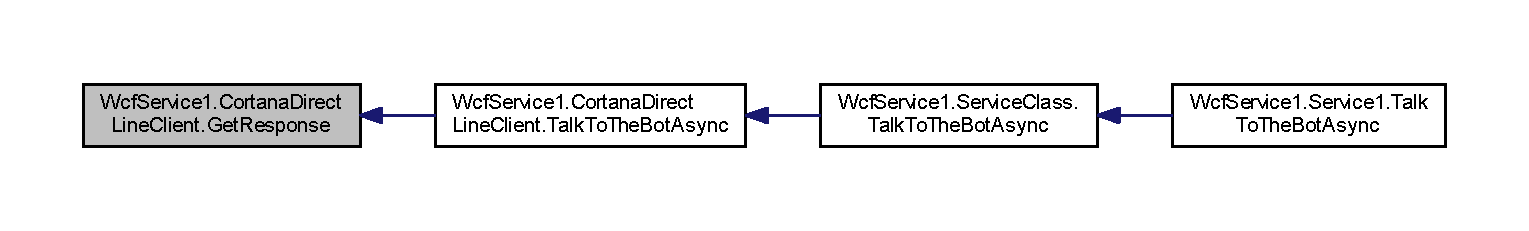
\includegraphics[width=350pt]{class_wcf_service1_1_1_cortana_direct_line_client_a0bc2576ae50d7eafd2092bb9cf7e6f7c_icgraph}
\end{center}
\end{figure}


\index{Wcf\+Service1\+::\+Cortana\+Direct\+Line\+Client@{Wcf\+Service1\+::\+Cortana\+Direct\+Line\+Client}!Talk\+To\+The\+Bot\+Async@{Talk\+To\+The\+Bot\+Async}}
\index{Talk\+To\+The\+Bot\+Async@{Talk\+To\+The\+Bot\+Async}!Wcf\+Service1\+::\+Cortana\+Direct\+Line\+Client@{Wcf\+Service1\+::\+Cortana\+Direct\+Line\+Client}}
\subsubsection[{\texorpdfstring{Talk\+To\+The\+Bot\+Async(string message)}{TalkToTheBotAsync(string message)}}]{\setlength{\rightskip}{0pt plus 5cm}async Task$<$string$>$ Wcf\+Service1.\+Cortana\+Direct\+Line\+Client.\+Talk\+To\+The\+Bot\+Async (
\begin{DoxyParamCaption}
\item[{string}]{message}
\end{DoxyParamCaption}
)}\hypertarget{class_wcf_service1_1_1_cortana_direct_line_client_ad9aee7d49dab0e3bb8806349b68716b3}{}\label{class_wcf_service1_1_1_cortana_direct_line_client_ad9aee7d49dab0e3bb8806349b68716b3}


sends a message to the bot and retrieves da response for it 


\begin{DoxyParams}{Parameters}
{\em message} & \\
\hline
\end{DoxyParams}
\begin{DoxyReturn}{Returns}

\end{DoxyReturn}


Here is the call graph for this function\+:\nopagebreak
\begin{figure}[H]
\begin{center}
\leavevmode
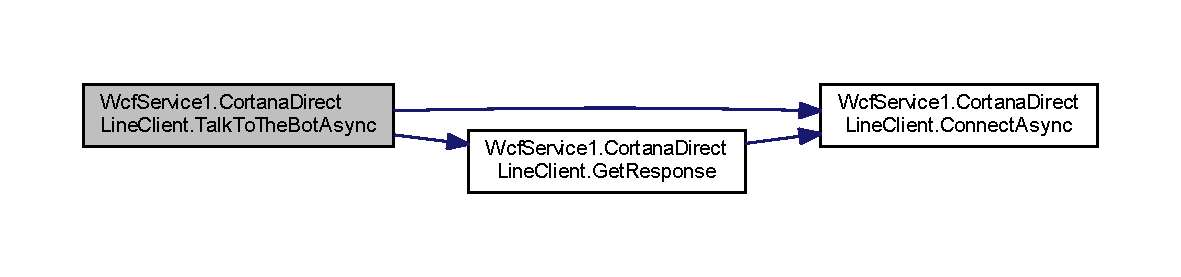
\includegraphics[width=350pt]{class_wcf_service1_1_1_cortana_direct_line_client_ad9aee7d49dab0e3bb8806349b68716b3_cgraph}
\end{center}
\end{figure}




Here is the caller graph for this function\+:\nopagebreak
\begin{figure}[H]
\begin{center}
\leavevmode
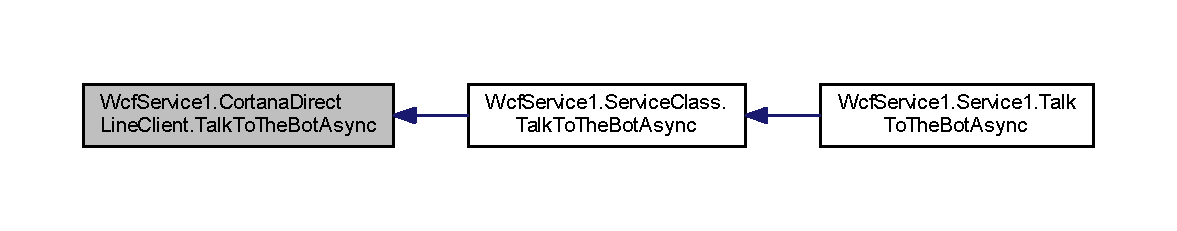
\includegraphics[width=350pt]{class_wcf_service1_1_1_cortana_direct_line_client_ad9aee7d49dab0e3bb8806349b68716b3_icgraph}
\end{center}
\end{figure}




\subsection{Member Data Documentation}
\index{Wcf\+Service1\+::\+Cortana\+Direct\+Line\+Client@{Wcf\+Service1\+::\+Cortana\+Direct\+Line\+Client}!\+\_\+conversation\+Id@{\+\_\+conversation\+Id}}
\index{\+\_\+conversation\+Id@{\+\_\+conversation\+Id}!Wcf\+Service1\+::\+Cortana\+Direct\+Line\+Client@{Wcf\+Service1\+::\+Cortana\+Direct\+Line\+Client}}
\subsubsection[{\texorpdfstring{\+\_\+conversation\+Id}{_conversationId}}]{\setlength{\rightskip}{0pt plus 5cm}string Wcf\+Service1.\+Cortana\+Direct\+Line\+Client.\+\_\+conversation\+Id\hspace{0.3cm}{\ttfamily [private]}}\hypertarget{class_wcf_service1_1_1_cortana_direct_line_client_a460c7a68d595773d131142651fa2b213}{}\label{class_wcf_service1_1_1_cortana_direct_line_client_a460c7a68d595773d131142651fa2b213}


client\textquotesingle{}s conversation id 

\index{Wcf\+Service1\+::\+Cortana\+Direct\+Line\+Client@{Wcf\+Service1\+::\+Cortana\+Direct\+Line\+Client}!\+\_\+direct\+Line@{\+\_\+direct\+Line}}
\index{\+\_\+direct\+Line@{\+\_\+direct\+Line}!Wcf\+Service1\+::\+Cortana\+Direct\+Line\+Client@{Wcf\+Service1\+::\+Cortana\+Direct\+Line\+Client}}
\subsubsection[{\texorpdfstring{\+\_\+direct\+Line}{_directLine}}]{\setlength{\rightskip}{0pt plus 5cm}Direct\+Line\+Client Wcf\+Service1.\+Cortana\+Direct\+Line\+Client.\+\_\+direct\+Line\hspace{0.3cm}{\ttfamily [private]}}\hypertarget{class_wcf_service1_1_1_cortana_direct_line_client_a2161a12a94efe732c80a2f31f7a91d8d}{}\label{class_wcf_service1_1_1_cortana_direct_line_client_a2161a12a94efe732c80a2f31f7a91d8d}


client 

\index{Wcf\+Service1\+::\+Cortana\+Direct\+Line\+Client@{Wcf\+Service1\+::\+Cortana\+Direct\+Line\+Client}!\+\_\+direct\+Line\+Secret@{\+\_\+direct\+Line\+Secret}}
\index{\+\_\+direct\+Line\+Secret@{\+\_\+direct\+Line\+Secret}!Wcf\+Service1\+::\+Cortana\+Direct\+Line\+Client@{Wcf\+Service1\+::\+Cortana\+Direct\+Line\+Client}}
\subsubsection[{\texorpdfstring{\+\_\+direct\+Line\+Secret}{_directLineSecret}}]{\setlength{\rightskip}{0pt plus 5cm}string Wcf\+Service1.\+Cortana\+Direct\+Line\+Client.\+\_\+direct\+Line\+Secret = Configuration\+Manager.\+App\+Settings\mbox{[}\char`\"{}Direct\+Line\+Secret\char`\"{}\mbox{]}\hspace{0.3cm}{\ttfamily [private]}}\hypertarget{class_wcf_service1_1_1_cortana_direct_line_client_a06b449cbb20e2a97dc873b306371b577}{}\label{class_wcf_service1_1_1_cortana_direct_line_client_a06b449cbb20e2a97dc873b306371b577}


the key to the bot\textquotesingle{}s Direct\+Line channel 

\index{Wcf\+Service1\+::\+Cortana\+Direct\+Line\+Client@{Wcf\+Service1\+::\+Cortana\+Direct\+Line\+Client}!bot\+Id@{bot\+Id}}
\index{bot\+Id@{bot\+Id}!Wcf\+Service1\+::\+Cortana\+Direct\+Line\+Client@{Wcf\+Service1\+::\+Cortana\+Direct\+Line\+Client}}
\subsubsection[{\texorpdfstring{bot\+Id}{botId}}]{\setlength{\rightskip}{0pt plus 5cm}string Wcf\+Service1.\+Cortana\+Direct\+Line\+Client.\+bot\+Id = Configuration\+Manager.\+App\+Settings\mbox{[}\char`\"{}Bot\+Id\char`\"{}\mbox{]}\hspace{0.3cm}{\ttfamily [private]}}\hypertarget{class_wcf_service1_1_1_cortana_direct_line_client_a92b26da0f83e644653c3cd4f8c248b1b}{}\label{class_wcf_service1_1_1_cortana_direct_line_client_a92b26da0f83e644653c3cd4f8c248b1b}


the bot\textquotesingle{}s microsoft id 

\index{Wcf\+Service1\+::\+Cortana\+Direct\+Line\+Client@{Wcf\+Service1\+::\+Cortana\+Direct\+Line\+Client}!username@{username}}
\index{username@{username}!Wcf\+Service1\+::\+Cortana\+Direct\+Line\+Client@{Wcf\+Service1\+::\+Cortana\+Direct\+Line\+Client}}
\subsubsection[{\texorpdfstring{username}{username}}]{\setlength{\rightskip}{0pt plus 5cm}readonly string Wcf\+Service1.\+Cortana\+Direct\+Line\+Client.\+username = Configuration\+Manager.\+App\+Settings\mbox{[}\char`\"{}user\+Name\char`\"{}\mbox{]}\hspace{0.3cm}{\ttfamily [private]}}\hypertarget{class_wcf_service1_1_1_cortana_direct_line_client_a5c02c54f3f2ed0d5c508092e516cb5d9}{}\label{class_wcf_service1_1_1_cortana_direct_line_client_a5c02c54f3f2ed0d5c508092e516cb5d9}


The documentation for this class was generated from the following file\+:\begin{DoxyCompactItemize}
\item 
C\+:/\+Users/user/source/repos/\+Hoermirzu/\+Listen\+To\+Me-\/master-\/89f0b49594deaade7bfad24dad062ff16eca36da/\+Wcf\+Service1/\hyperlink{_cortana_direct_line_client_8cs}{Cortana\+Direct\+Line\+Client.\+cs}\end{DoxyCompactItemize}

\hypertarget{class_wcf_service1_1_1_implementation___mock}{}\section{Wcf\+Service1.\+Implementation\+\_\+\+Mock Class Reference}
\label{class_wcf_service1_1_1_implementation___mock}\index{Wcf\+Service1.\+Implementation\+\_\+\+Mock@{Wcf\+Service1.\+Implementation\+\_\+\+Mock}}


Inheritance diagram for Wcf\+Service1.\+Implementation\+\_\+\+Mock\+:\nopagebreak
\begin{figure}[H]
\begin{center}
\leavevmode
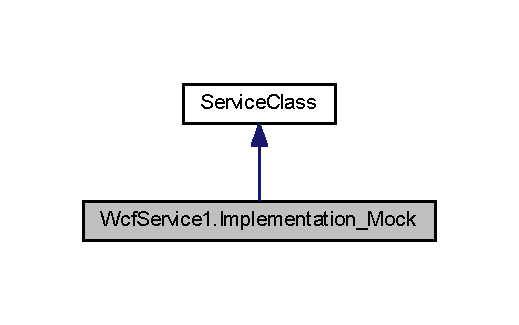
\includegraphics[width=249pt]{class_wcf_service1_1_1_implementation___mock__inherit__graph}
\end{center}
\end{figure}


Collaboration diagram for Wcf\+Service1.\+Implementation\+\_\+\+Mock\+:\nopagebreak
\begin{figure}[H]
\begin{center}
\leavevmode
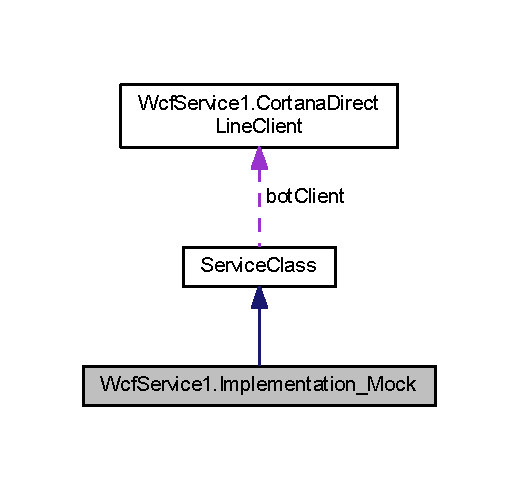
\includegraphics[width=249pt]{class_wcf_service1_1_1_implementation___mock__coll__graph}
\end{center}
\end{figure}
\subsection*{Public Member Functions}
\begin{DoxyCompactItemize}
\item 
Task \hyperlink{class_wcf_service1_1_1_implementation___mock_aeee2fcebb9cfd636b4ead332f500273c}{Connect\+Async} ()
\item 
override List$<$ Section $>$ \hyperlink{class_wcf_service1_1_1_implementation___mock_a3677cf44f7acac9549f1e58ce9191e4e}{Get\+All\+Elements} (string username, string password)
\item 
override string \hyperlink{class_wcf_service1_1_1_implementation___mock_a770d195f0883f20e2356381152a6ea00}{Get\+Form} (string username, string password)
\item 
override string \hyperlink{class_wcf_service1_1_1_implementation___mock_ad4676c509d48e01e7ed6e2962fc01b29}{Login} (string user\+Name, string password)
\item 
override bool \hyperlink{class_wcf_service1_1_1_implementation___mock_aacbbae5d5cd842b1c62cfab84168b287}{Upload\+Section} (Section section)
\end{DoxyCompactItemize}
\subsection*{Private Member Functions}
\begin{DoxyCompactItemize}
\item 
Section \hyperlink{class_wcf_service1_1_1_implementation___mock_a8cc683e1ef69f6d291c8b0381163d69b}{convert\+String\+To\+Section} (string section)
\begin{DoxyCompactList}\small\item\em processes the json string contained in the sections\+List into a Section from the Portable\+Class\+Library model \end{DoxyCompactList}\item 
string \hyperlink{class_wcf_service1_1_1_implementation___mock_a137882a409681590c57f58b259d1e6cb}{read\+File} (string path\+File)
\begin{DoxyCompactList}\small\item\em reads a text file (in this case json file) \end{DoxyCompactList}\end{DoxyCompactItemize}


\subsection{Member Function Documentation}
\index{Wcf\+Service1\+::\+Implementation\+\_\+\+Mock@{Wcf\+Service1\+::\+Implementation\+\_\+\+Mock}!Connect\+Async@{Connect\+Async}}
\index{Connect\+Async@{Connect\+Async}!Wcf\+Service1\+::\+Implementation\+\_\+\+Mock@{Wcf\+Service1\+::\+Implementation\+\_\+\+Mock}}
\subsubsection[{\texorpdfstring{Connect\+Async()}{ConnectAsync()}}]{\setlength{\rightskip}{0pt plus 5cm}Task Wcf\+Service1.\+Implementation\+\_\+\+Mock.\+Connect\+Async (
\begin{DoxyParamCaption}
{}
\end{DoxyParamCaption}
)}\hypertarget{class_wcf_service1_1_1_implementation___mock_aeee2fcebb9cfd636b4ead332f500273c}{}\label{class_wcf_service1_1_1_implementation___mock_aeee2fcebb9cfd636b4ead332f500273c}
\index{Wcf\+Service1\+::\+Implementation\+\_\+\+Mock@{Wcf\+Service1\+::\+Implementation\+\_\+\+Mock}!convert\+String\+To\+Section@{convert\+String\+To\+Section}}
\index{convert\+String\+To\+Section@{convert\+String\+To\+Section}!Wcf\+Service1\+::\+Implementation\+\_\+\+Mock@{Wcf\+Service1\+::\+Implementation\+\_\+\+Mock}}
\subsubsection[{\texorpdfstring{convert\+String\+To\+Section(string section)}{convertStringToSection(string section)}}]{\setlength{\rightskip}{0pt plus 5cm}Section Wcf\+Service1.\+Implementation\+\_\+\+Mock.\+convert\+String\+To\+Section (
\begin{DoxyParamCaption}
\item[{string}]{section}
\end{DoxyParamCaption}
)\hspace{0.3cm}{\ttfamily [private]}}\hypertarget{class_wcf_service1_1_1_implementation___mock_a8cc683e1ef69f6d291c8b0381163d69b}{}\label{class_wcf_service1_1_1_implementation___mock_a8cc683e1ef69f6d291c8b0381163d69b}


processes the json string contained in the sections\+List into a Section from the Portable\+Class\+Library model 


\begin{DoxyParams}{Parameters}
{\em section} & \\
\hline
\end{DoxyParams}
\begin{DoxyReturn}{Returns}

\end{DoxyReturn}


Here is the caller graph for this function\+:\nopagebreak
\begin{figure}[H]
\begin{center}
\leavevmode
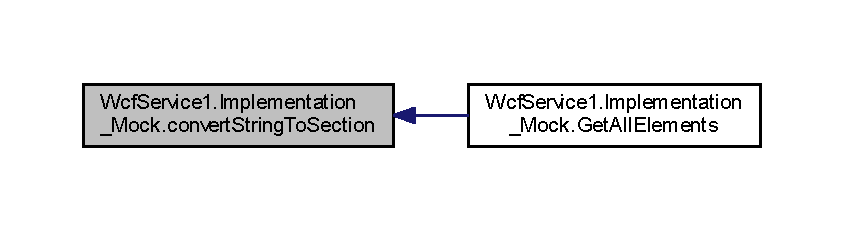
\includegraphics[width=350pt]{class_wcf_service1_1_1_implementation___mock_a8cc683e1ef69f6d291c8b0381163d69b_icgraph}
\end{center}
\end{figure}


\index{Wcf\+Service1\+::\+Implementation\+\_\+\+Mock@{Wcf\+Service1\+::\+Implementation\+\_\+\+Mock}!Get\+All\+Elements@{Get\+All\+Elements}}
\index{Get\+All\+Elements@{Get\+All\+Elements}!Wcf\+Service1\+::\+Implementation\+\_\+\+Mock@{Wcf\+Service1\+::\+Implementation\+\_\+\+Mock}}
\subsubsection[{\texorpdfstring{Get\+All\+Elements(string username, string password)}{GetAllElements(string username, string password)}}]{\setlength{\rightskip}{0pt plus 5cm}override List$<$Section$>$ Wcf\+Service1.\+Implementation\+\_\+\+Mock.\+Get\+All\+Elements (
\begin{DoxyParamCaption}
\item[{string}]{username, }
\item[{string}]{password}
\end{DoxyParamCaption}
)\hspace{0.3cm}{\ttfamily [virtual]}}\hypertarget{class_wcf_service1_1_1_implementation___mock_a3677cf44f7acac9549f1e58ce9191e4e}{}\label{class_wcf_service1_1_1_implementation___mock_a3677cf44f7acac9549f1e58ce9191e4e}


Implements \hyperlink{class_wcf_service1_1_1_service_class_ac0640daeb28fada4b6f80a2b66b0ec3e}{Wcf\+Service1.\+Service\+Class}.



Here is the call graph for this function\+:\nopagebreak
\begin{figure}[H]
\begin{center}
\leavevmode
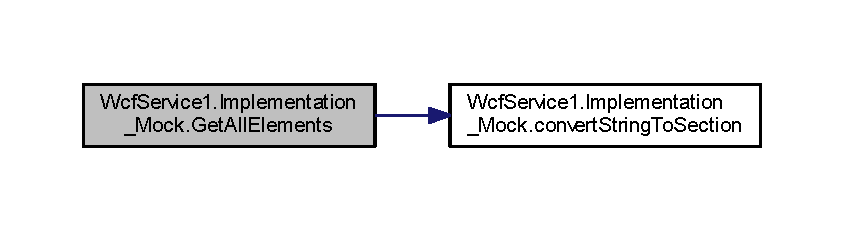
\includegraphics[width=350pt]{class_wcf_service1_1_1_implementation___mock_a3677cf44f7acac9549f1e58ce9191e4e_cgraph}
\end{center}
\end{figure}


\index{Wcf\+Service1\+::\+Implementation\+\_\+\+Mock@{Wcf\+Service1\+::\+Implementation\+\_\+\+Mock}!Get\+Form@{Get\+Form}}
\index{Get\+Form@{Get\+Form}!Wcf\+Service1\+::\+Implementation\+\_\+\+Mock@{Wcf\+Service1\+::\+Implementation\+\_\+\+Mock}}
\subsubsection[{\texorpdfstring{Get\+Form(string username, string password)}{GetForm(string username, string password)}}]{\setlength{\rightskip}{0pt plus 5cm}override string Wcf\+Service1.\+Implementation\+\_\+\+Mock.\+Get\+Form (
\begin{DoxyParamCaption}
\item[{string}]{username, }
\item[{string}]{password}
\end{DoxyParamCaption}
)\hspace{0.3cm}{\ttfamily [virtual]}}\hypertarget{class_wcf_service1_1_1_implementation___mock_a770d195f0883f20e2356381152a6ea00}{}\label{class_wcf_service1_1_1_implementation___mock_a770d195f0883f20e2356381152a6ea00}


Implements \hyperlink{class_wcf_service1_1_1_service_class_a791350c6bf7ba90f63f95e1b935dde3b}{Wcf\+Service1.\+Service\+Class}.



Here is the call graph for this function\+:\nopagebreak
\begin{figure}[H]
\begin{center}
\leavevmode
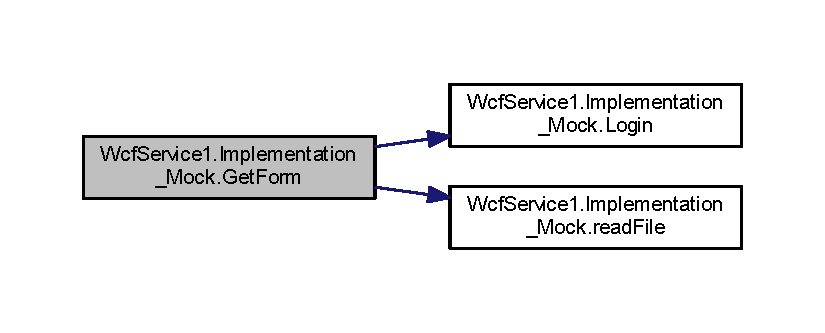
\includegraphics[width=350pt]{class_wcf_service1_1_1_implementation___mock_a770d195f0883f20e2356381152a6ea00_cgraph}
\end{center}
\end{figure}


\index{Wcf\+Service1\+::\+Implementation\+\_\+\+Mock@{Wcf\+Service1\+::\+Implementation\+\_\+\+Mock}!Login@{Login}}
\index{Login@{Login}!Wcf\+Service1\+::\+Implementation\+\_\+\+Mock@{Wcf\+Service1\+::\+Implementation\+\_\+\+Mock}}
\subsubsection[{\texorpdfstring{Login(string user\+Name, string password)}{Login(string userName, string password)}}]{\setlength{\rightskip}{0pt plus 5cm}override string Wcf\+Service1.\+Implementation\+\_\+\+Mock.\+Login (
\begin{DoxyParamCaption}
\item[{string}]{user\+Name, }
\item[{string}]{password}
\end{DoxyParamCaption}
)\hspace{0.3cm}{\ttfamily [virtual]}}\hypertarget{class_wcf_service1_1_1_implementation___mock_ad4676c509d48e01e7ed6e2962fc01b29}{}\label{class_wcf_service1_1_1_implementation___mock_ad4676c509d48e01e7ed6e2962fc01b29}


Implements \hyperlink{class_wcf_service1_1_1_service_class_a023c63c6a95132c7f2b9754c1bb41c80}{Wcf\+Service1.\+Service\+Class}.



Here is the caller graph for this function\+:\nopagebreak
\begin{figure}[H]
\begin{center}
\leavevmode
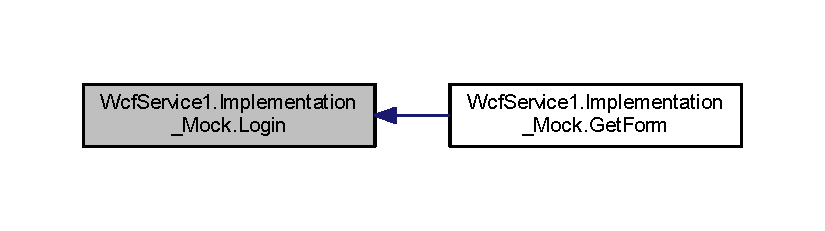
\includegraphics[width=350pt]{class_wcf_service1_1_1_implementation___mock_ad4676c509d48e01e7ed6e2962fc01b29_icgraph}
\end{center}
\end{figure}


\index{Wcf\+Service1\+::\+Implementation\+\_\+\+Mock@{Wcf\+Service1\+::\+Implementation\+\_\+\+Mock}!read\+File@{read\+File}}
\index{read\+File@{read\+File}!Wcf\+Service1\+::\+Implementation\+\_\+\+Mock@{Wcf\+Service1\+::\+Implementation\+\_\+\+Mock}}
\subsubsection[{\texorpdfstring{read\+File(string path\+File)}{readFile(string pathFile)}}]{\setlength{\rightskip}{0pt plus 5cm}string Wcf\+Service1.\+Implementation\+\_\+\+Mock.\+read\+File (
\begin{DoxyParamCaption}
\item[{string}]{path\+File}
\end{DoxyParamCaption}
)\hspace{0.3cm}{\ttfamily [private]}}\hypertarget{class_wcf_service1_1_1_implementation___mock_a137882a409681590c57f58b259d1e6cb}{}\label{class_wcf_service1_1_1_implementation___mock_a137882a409681590c57f58b259d1e6cb}


reads a text file (in this case json file) 


\begin{DoxyParams}{Parameters}
{\em path\+File} & \\
\hline
\end{DoxyParams}
\begin{DoxyReturn}{Returns}
the content of the file
\end{DoxyReturn}


Here is the caller graph for this function\+:\nopagebreak
\begin{figure}[H]
\begin{center}
\leavevmode
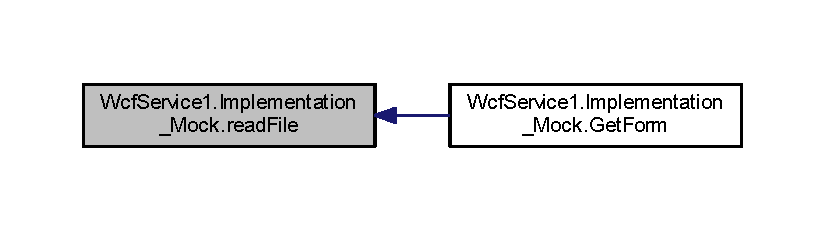
\includegraphics[width=350pt]{class_wcf_service1_1_1_implementation___mock_a137882a409681590c57f58b259d1e6cb_icgraph}
\end{center}
\end{figure}


\index{Wcf\+Service1\+::\+Implementation\+\_\+\+Mock@{Wcf\+Service1\+::\+Implementation\+\_\+\+Mock}!Upload\+Section@{Upload\+Section}}
\index{Upload\+Section@{Upload\+Section}!Wcf\+Service1\+::\+Implementation\+\_\+\+Mock@{Wcf\+Service1\+::\+Implementation\+\_\+\+Mock}}
\subsubsection[{\texorpdfstring{Upload\+Section(\+Section section)}{UploadSection(Section section)}}]{\setlength{\rightskip}{0pt plus 5cm}override bool Wcf\+Service1.\+Implementation\+\_\+\+Mock.\+Upload\+Section (
\begin{DoxyParamCaption}
\item[{Section}]{section}
\end{DoxyParamCaption}
)\hspace{0.3cm}{\ttfamily [virtual]}}\hypertarget{class_wcf_service1_1_1_implementation___mock_aacbbae5d5cd842b1c62cfab84168b287}{}\label{class_wcf_service1_1_1_implementation___mock_aacbbae5d5cd842b1c62cfab84168b287}


Implements \hyperlink{class_wcf_service1_1_1_service_class_add477e49eab8927cc943dfb751dc976a}{Wcf\+Service1.\+Service\+Class}.



The documentation for this class was generated from the following file\+:\begin{DoxyCompactItemize}
\item 
C\+:/\+Users/user/source/repos/\+Hoermirzu/\+Listen\+To\+Me-\/master-\/89f0b49594deaade7bfad24dad062ff16eca36da/\+Wcf\+Service1/\hyperlink{_implementation___mock_8cs}{Implementation\+\_\+\+Mock.\+cs}\end{DoxyCompactItemize}

\hypertarget{class_wcf_service1_1_1_implementation___real}{}\section{Wcf\+Service1.\+Implementation\+\_\+\+Real Class Reference}
\label{class_wcf_service1_1_1_implementation___real}\index{Wcf\+Service1.\+Implementation\+\_\+\+Real@{Wcf\+Service1.\+Implementation\+\_\+\+Real}}


Inheritance diagram for Wcf\+Service1.\+Implementation\+\_\+\+Real\+:\nopagebreak
\begin{figure}[H]
\begin{center}
\leavevmode
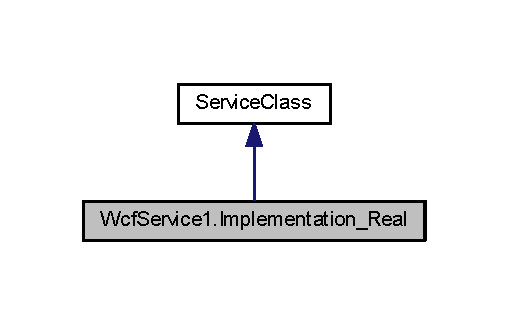
\includegraphics[width=244pt]{class_wcf_service1_1_1_implementation___real__inherit__graph}
\end{center}
\end{figure}


Collaboration diagram for Wcf\+Service1.\+Implementation\+\_\+\+Real\+:\nopagebreak
\begin{figure}[H]
\begin{center}
\leavevmode
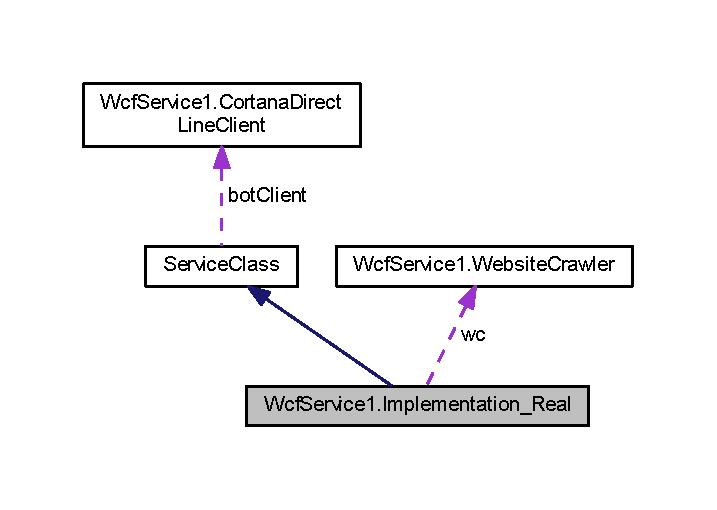
\includegraphics[width=344pt]{class_wcf_service1_1_1_implementation___real__coll__graph}
\end{center}
\end{figure}
\subsection*{Public Member Functions}
\begin{DoxyCompactItemize}
\item 
override List$<$ Section $>$ \hyperlink{class_wcf_service1_1_1_implementation___real_a6cedd1da2b421038727ed52afaf7197e}{Get\+All\+Elements} (string username, string password)
\item 
override string \hyperlink{class_wcf_service1_1_1_implementation___real_a82b0d0cc9a634454bfa583f55eb13dad}{Get\+Form} (string username, string password)
\item 
override string \hyperlink{class_wcf_service1_1_1_implementation___real_aec1081c3a83135e9f11ea182ca3e9321}{Login} (string user\+Name, string password)
\item 
override bool \hyperlink{class_wcf_service1_1_1_implementation___real_ac95892552f6beb92e0557abde468a5a1}{Upload\+Section} (Section section)
\end{DoxyCompactItemize}
\subsection*{Private Member Functions}
\begin{DoxyCompactItemize}
\item 
void \hyperlink{class_wcf_service1_1_1_implementation___real_a15223fee34324eadbaf60510013d78c0}{cut\+Leading\+Number\+From\+Heading} (Element element)
\item 
string \hyperlink{class_wcf_service1_1_1_implementation___real_a79882899922f4204592c464a2cb6a71d}{Clean\+String\+From\+H\+T\+ML} (string to\+Clean)
\begin{DoxyCompactList}\small\item\em cleans a text from Htlm decoded values. I found that Http\+Utility.\+Decode() is not working on this correctly, when there are two \& \textquotesingle{}s behind each other as in the patterns sometimes the caase reference\+: \href{http://weblogs.sqlteam.com/mladenp/archive/2008/10/21/Different-ways-how-to-escape-an-XML-string-in-C.aspx}{\tt http\+://weblogs.\+sqlteam.\+com/mladenp/archive/2008/10/21/\+Different-\/ways-\/how-\/to-\/escape-\/an-\/\+X\+M\+L-\/string-\/in-\/\+C.\+aspx} \end{DoxyCompactList}\item 
Html\+Node \hyperlink{class_wcf_service1_1_1_implementation___real_ac320b296695abc0db1ff6266f7d39dda}{select\+Child\+Node} (Html\+Node node)
\begin{DoxyCompactList}\small\item\em selects a specific child node from the dropdown list node \end{DoxyCompactList}\end{DoxyCompactItemize}
\subsection*{Private Attributes}
\begin{DoxyCompactItemize}
\item 
\hyperlink{class_wcf_service1_1_1_website_crawler}{Website\+Crawler} \hyperlink{class_wcf_service1_1_1_implementation___real_a670aed6bbd357da19134e8f8c3c907a9}{wc} = new \hyperlink{class_wcf_service1_1_1_website_crawler}{Website\+Crawler}()
\begin{DoxyCompactList}\small\item\em the headless browser used to connect to the form. \end{DoxyCompactList}\end{DoxyCompactItemize}


\subsection{Member Function Documentation}
\index{Wcf\+Service1\+::\+Implementation\+\_\+\+Real@{Wcf\+Service1\+::\+Implementation\+\_\+\+Real}!Clean\+String\+From\+H\+T\+ML@{Clean\+String\+From\+H\+T\+ML}}
\index{Clean\+String\+From\+H\+T\+ML@{Clean\+String\+From\+H\+T\+ML}!Wcf\+Service1\+::\+Implementation\+\_\+\+Real@{Wcf\+Service1\+::\+Implementation\+\_\+\+Real}}
\subsubsection[{\texorpdfstring{Clean\+String\+From\+H\+T\+M\+L(string to\+Clean)}{CleanStringFromHTML(string toClean)}}]{\setlength{\rightskip}{0pt plus 5cm}string Wcf\+Service1.\+Implementation\+\_\+\+Real.\+Clean\+String\+From\+H\+T\+ML (
\begin{DoxyParamCaption}
\item[{string}]{to\+Clean}
\end{DoxyParamCaption}
)\hspace{0.3cm}{\ttfamily [private]}}\hypertarget{class_wcf_service1_1_1_implementation___real_a79882899922f4204592c464a2cb6a71d}{}\label{class_wcf_service1_1_1_implementation___real_a79882899922f4204592c464a2cb6a71d}


cleans a text from Htlm decoded values. I found that Http\+Utility.\+Decode() is not working on this correctly, when there are two \& \textquotesingle{}s behind each other as in the patterns sometimes the caase reference\+: \href{http://weblogs.sqlteam.com/mladenp/archive/2008/10/21/Different-ways-how-to-escape-an-XML-string-in-C.aspx}{\tt http\+://weblogs.\+sqlteam.\+com/mladenp/archive/2008/10/21/\+Different-\/ways-\/how-\/to-\/escape-\/an-\/\+X\+M\+L-\/string-\/in-\/\+C.\+aspx} 


\begin{DoxyParams}{Parameters}
{\em to\+Clean} & \\
\hline
\end{DoxyParams}
\begin{DoxyReturn}{Returns}

\end{DoxyReturn}


Here is the caller graph for this function\+:\nopagebreak
\begin{figure}[H]
\begin{center}
\leavevmode
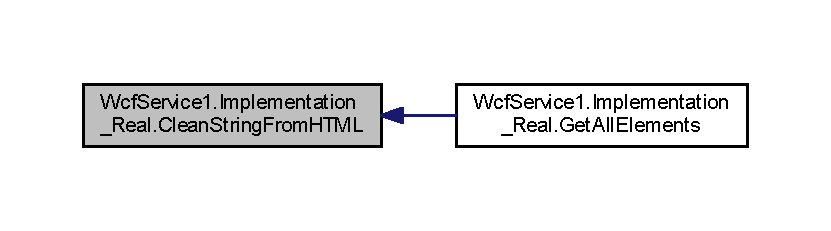
\includegraphics[width=350pt]{class_wcf_service1_1_1_implementation___real_a79882899922f4204592c464a2cb6a71d_icgraph}
\end{center}
\end{figure}


\index{Wcf\+Service1\+::\+Implementation\+\_\+\+Real@{Wcf\+Service1\+::\+Implementation\+\_\+\+Real}!cut\+Leading\+Number\+From\+Heading@{cut\+Leading\+Number\+From\+Heading}}
\index{cut\+Leading\+Number\+From\+Heading@{cut\+Leading\+Number\+From\+Heading}!Wcf\+Service1\+::\+Implementation\+\_\+\+Real@{Wcf\+Service1\+::\+Implementation\+\_\+\+Real}}
\subsubsection[{\texorpdfstring{cut\+Leading\+Number\+From\+Heading(\+Element element)}{cutLeadingNumberFromHeading(Element element)}}]{\setlength{\rightskip}{0pt plus 5cm}void Wcf\+Service1.\+Implementation\+\_\+\+Real.\+cut\+Leading\+Number\+From\+Heading (
\begin{DoxyParamCaption}
\item[{Element}]{element}
\end{DoxyParamCaption}
)\hspace{0.3cm}{\ttfamily [private]}}\hypertarget{class_wcf_service1_1_1_implementation___real_a15223fee34324eadbaf60510013d78c0}{}\label{class_wcf_service1_1_1_implementation___real_a15223fee34324eadbaf60510013d78c0}


Here is the caller graph for this function\+:\nopagebreak
\begin{figure}[H]
\begin{center}
\leavevmode
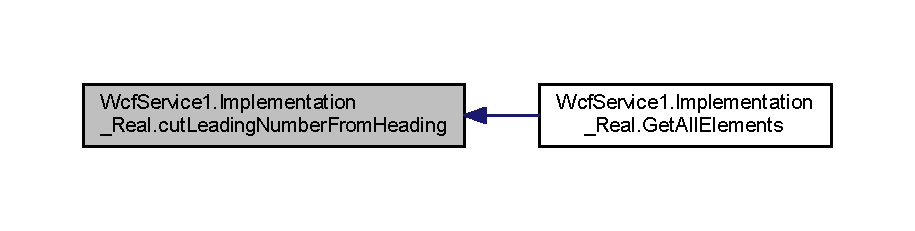
\includegraphics[width=350pt]{class_wcf_service1_1_1_implementation___real_a15223fee34324eadbaf60510013d78c0_icgraph}
\end{center}
\end{figure}


\index{Wcf\+Service1\+::\+Implementation\+\_\+\+Real@{Wcf\+Service1\+::\+Implementation\+\_\+\+Real}!Get\+All\+Elements@{Get\+All\+Elements}}
\index{Get\+All\+Elements@{Get\+All\+Elements}!Wcf\+Service1\+::\+Implementation\+\_\+\+Real@{Wcf\+Service1\+::\+Implementation\+\_\+\+Real}}
\subsubsection[{\texorpdfstring{Get\+All\+Elements(string username, string password)}{GetAllElements(string username, string password)}}]{\setlength{\rightskip}{0pt plus 5cm}override List$<$Section$>$ Wcf\+Service1.\+Implementation\+\_\+\+Real.\+Get\+All\+Elements (
\begin{DoxyParamCaption}
\item[{string}]{username, }
\item[{string}]{password}
\end{DoxyParamCaption}
)\hspace{0.3cm}{\ttfamily [virtual]}}\hypertarget{class_wcf_service1_1_1_implementation___real_a6cedd1da2b421038727ed52afaf7197e}{}\label{class_wcf_service1_1_1_implementation___real_a6cedd1da2b421038727ed52afaf7197e}
string.\+Is\+Null\+Or\+White\+Space(element.\+Text)\&\& 

Implements \hyperlink{class_wcf_service1_1_1_service_class_ac0640daeb28fada4b6f80a2b66b0ec3e}{Wcf\+Service1.\+Service\+Class}.



Here is the call graph for this function\+:\nopagebreak
\begin{figure}[H]
\begin{center}
\leavevmode
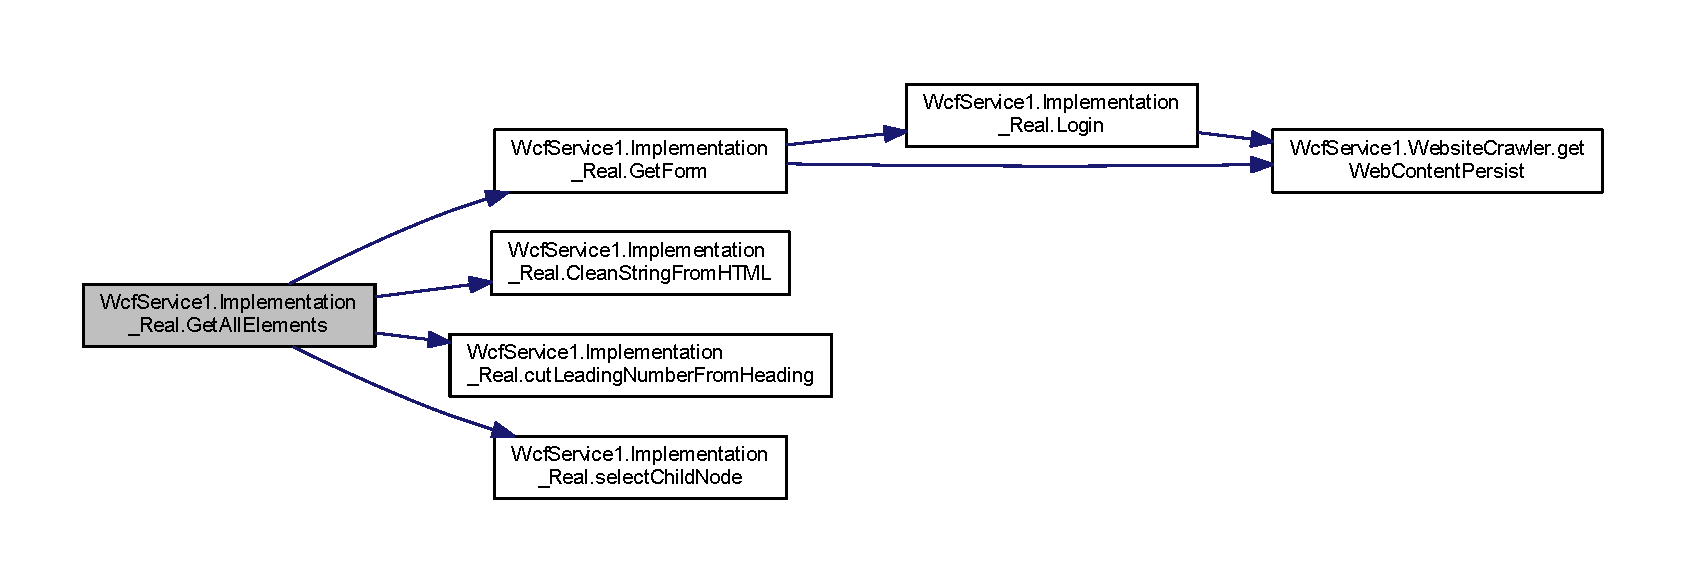
\includegraphics[width=350pt]{class_wcf_service1_1_1_implementation___real_a6cedd1da2b421038727ed52afaf7197e_cgraph}
\end{center}
\end{figure}


\index{Wcf\+Service1\+::\+Implementation\+\_\+\+Real@{Wcf\+Service1\+::\+Implementation\+\_\+\+Real}!Get\+Form@{Get\+Form}}
\index{Get\+Form@{Get\+Form}!Wcf\+Service1\+::\+Implementation\+\_\+\+Real@{Wcf\+Service1\+::\+Implementation\+\_\+\+Real}}
\subsubsection[{\texorpdfstring{Get\+Form(string username, string password)}{GetForm(string username, string password)}}]{\setlength{\rightskip}{0pt plus 5cm}override string Wcf\+Service1.\+Implementation\+\_\+\+Real.\+Get\+Form (
\begin{DoxyParamCaption}
\item[{string}]{username, }
\item[{string}]{password}
\end{DoxyParamCaption}
)\hspace{0.3cm}{\ttfamily [virtual]}}\hypertarget{class_wcf_service1_1_1_implementation___real_a82b0d0cc9a634454bfa583f55eb13dad}{}\label{class_wcf_service1_1_1_implementation___real_a82b0d0cc9a634454bfa583f55eb13dad}


Implements \hyperlink{class_wcf_service1_1_1_service_class_a791350c6bf7ba90f63f95e1b935dde3b}{Wcf\+Service1.\+Service\+Class}.



Here is the call graph for this function\+:\nopagebreak
\begin{figure}[H]
\begin{center}
\leavevmode
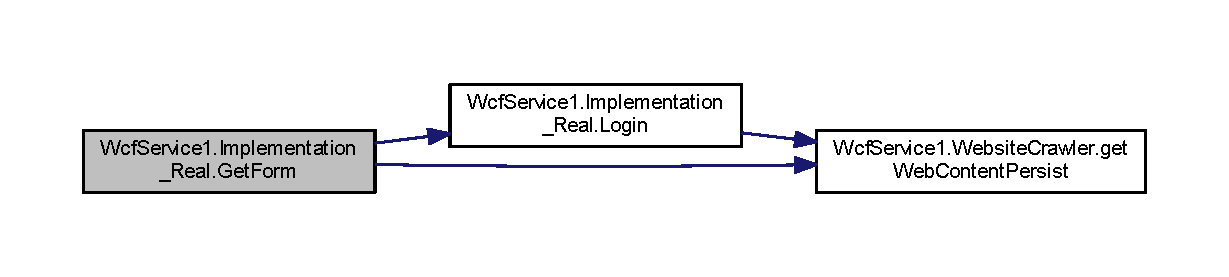
\includegraphics[width=350pt]{class_wcf_service1_1_1_implementation___real_a82b0d0cc9a634454bfa583f55eb13dad_cgraph}
\end{center}
\end{figure}




Here is the caller graph for this function\+:\nopagebreak
\begin{figure}[H]
\begin{center}
\leavevmode
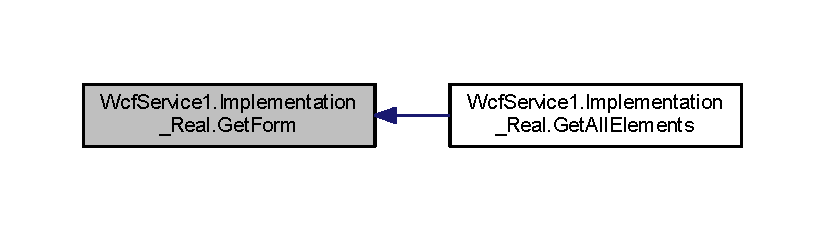
\includegraphics[width=350pt]{class_wcf_service1_1_1_implementation___real_a82b0d0cc9a634454bfa583f55eb13dad_icgraph}
\end{center}
\end{figure}


\index{Wcf\+Service1\+::\+Implementation\+\_\+\+Real@{Wcf\+Service1\+::\+Implementation\+\_\+\+Real}!Login@{Login}}
\index{Login@{Login}!Wcf\+Service1\+::\+Implementation\+\_\+\+Real@{Wcf\+Service1\+::\+Implementation\+\_\+\+Real}}
\subsubsection[{\texorpdfstring{Login(string user\+Name, string password)}{Login(string userName, string password)}}]{\setlength{\rightskip}{0pt plus 5cm}override string Wcf\+Service1.\+Implementation\+\_\+\+Real.\+Login (
\begin{DoxyParamCaption}
\item[{string}]{user\+Name, }
\item[{string}]{password}
\end{DoxyParamCaption}
)\hspace{0.3cm}{\ttfamily [virtual]}}\hypertarget{class_wcf_service1_1_1_implementation___real_aec1081c3a83135e9f11ea182ca3e9321}{}\label{class_wcf_service1_1_1_implementation___real_aec1081c3a83135e9f11ea182ca3e9321}


Implements \hyperlink{class_wcf_service1_1_1_service_class_a023c63c6a95132c7f2b9754c1bb41c80}{Wcf\+Service1.\+Service\+Class}.



Here is the call graph for this function\+:\nopagebreak
\begin{figure}[H]
\begin{center}
\leavevmode
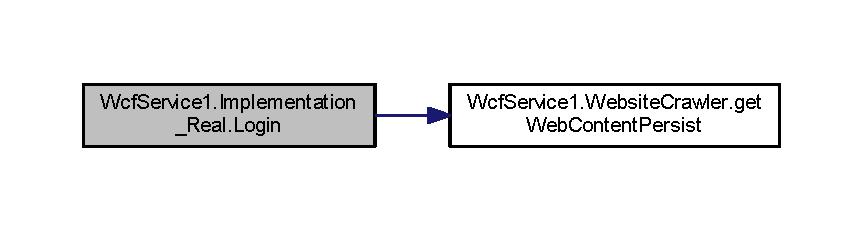
\includegraphics[width=350pt]{class_wcf_service1_1_1_implementation___real_aec1081c3a83135e9f11ea182ca3e9321_cgraph}
\end{center}
\end{figure}




Here is the caller graph for this function\+:\nopagebreak
\begin{figure}[H]
\begin{center}
\leavevmode
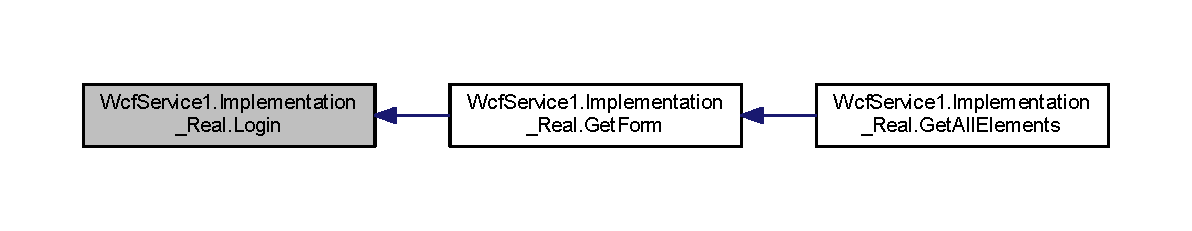
\includegraphics[width=350pt]{class_wcf_service1_1_1_implementation___real_aec1081c3a83135e9f11ea182ca3e9321_icgraph}
\end{center}
\end{figure}


\index{Wcf\+Service1\+::\+Implementation\+\_\+\+Real@{Wcf\+Service1\+::\+Implementation\+\_\+\+Real}!select\+Child\+Node@{select\+Child\+Node}}
\index{select\+Child\+Node@{select\+Child\+Node}!Wcf\+Service1\+::\+Implementation\+\_\+\+Real@{Wcf\+Service1\+::\+Implementation\+\_\+\+Real}}
\subsubsection[{\texorpdfstring{select\+Child\+Node(\+Html\+Node node)}{selectChildNode(HtmlNode node)}}]{\setlength{\rightskip}{0pt plus 5cm}Html\+Node Wcf\+Service1.\+Implementation\+\_\+\+Real.\+select\+Child\+Node (
\begin{DoxyParamCaption}
\item[{Html\+Node}]{node}
\end{DoxyParamCaption}
)\hspace{0.3cm}{\ttfamily [private]}}\hypertarget{class_wcf_service1_1_1_implementation___real_ac320b296695abc0db1ff6266f7d39dda}{}\label{class_wcf_service1_1_1_implementation___real_ac320b296695abc0db1ff6266f7d39dda}


selects a specific child node from the dropdown list node 


\begin{DoxyParams}{Parameters}
{\em node} & \\
\hline
\end{DoxyParams}
\begin{DoxyReturn}{Returns}

\end{DoxyReturn}


Here is the caller graph for this function\+:\nopagebreak
\begin{figure}[H]
\begin{center}
\leavevmode
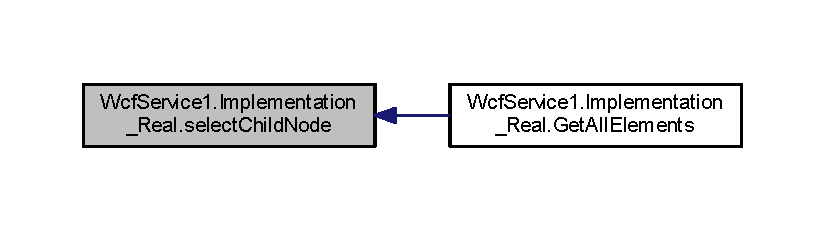
\includegraphics[width=350pt]{class_wcf_service1_1_1_implementation___real_ac320b296695abc0db1ff6266f7d39dda_icgraph}
\end{center}
\end{figure}


\index{Wcf\+Service1\+::\+Implementation\+\_\+\+Real@{Wcf\+Service1\+::\+Implementation\+\_\+\+Real}!Upload\+Section@{Upload\+Section}}
\index{Upload\+Section@{Upload\+Section}!Wcf\+Service1\+::\+Implementation\+\_\+\+Real@{Wcf\+Service1\+::\+Implementation\+\_\+\+Real}}
\subsubsection[{\texorpdfstring{Upload\+Section(\+Section section)}{UploadSection(Section section)}}]{\setlength{\rightskip}{0pt plus 5cm}override bool Wcf\+Service1.\+Implementation\+\_\+\+Real.\+Upload\+Section (
\begin{DoxyParamCaption}
\item[{Section}]{section}
\end{DoxyParamCaption}
)\hspace{0.3cm}{\ttfamily [virtual]}}\hypertarget{class_wcf_service1_1_1_implementation___real_ac95892552f6beb92e0557abde468a5a1}{}\label{class_wcf_service1_1_1_implementation___real_ac95892552f6beb92e0557abde468a5a1}


Implements \hyperlink{class_wcf_service1_1_1_service_class_add477e49eab8927cc943dfb751dc976a}{Wcf\+Service1.\+Service\+Class}.



\subsection{Member Data Documentation}
\index{Wcf\+Service1\+::\+Implementation\+\_\+\+Real@{Wcf\+Service1\+::\+Implementation\+\_\+\+Real}!wc@{wc}}
\index{wc@{wc}!Wcf\+Service1\+::\+Implementation\+\_\+\+Real@{Wcf\+Service1\+::\+Implementation\+\_\+\+Real}}
\subsubsection[{\texorpdfstring{wc}{wc}}]{\setlength{\rightskip}{0pt plus 5cm}{\bf Website\+Crawler} Wcf\+Service1.\+Implementation\+\_\+\+Real.\+wc = new {\bf Website\+Crawler}()\hspace{0.3cm}{\ttfamily [private]}}\hypertarget{class_wcf_service1_1_1_implementation___real_a670aed6bbd357da19134e8f8c3c907a9}{}\label{class_wcf_service1_1_1_implementation___real_a670aed6bbd357da19134e8f8c3c907a9}


the headless browser used to connect to the form. 



The documentation for this class was generated from the following file\+:\begin{DoxyCompactItemize}
\item 
C\+:/\+Users/user/source/repos/\+Hoermirzu/\+Listen\+To\+Me-\/master-\/89f0b49594deaade7bfad24dad062ff16eca36da/\+Wcf\+Service1/\hyperlink{_implementation___real_8cs}{Implementation\+\_\+\+Real.\+cs}\end{DoxyCompactItemize}

\hypertarget{class_wcf_service1_1_1_implementation_factory}{}\section{Wcf\+Service1.\+Implementation\+Factory Class Reference}
\label{class_wcf_service1_1_1_implementation_factory}\index{Wcf\+Service1.\+Implementation\+Factory@{Wcf\+Service1.\+Implementation\+Factory}}


reference\+: \href{http://www.c-sharpcorner.com/article/factory-method-design-pattern-in-c-sharp/}{\tt http\+://www.\+c-\/sharpcorner.\+com/article/factory-\/method-\/design-\/pattern-\/in-\/c-\/sharp/}  




Inheritance diagram for Wcf\+Service1.\+Implementation\+Factory\+:\nopagebreak
\begin{figure}[H]
\begin{center}
\leavevmode
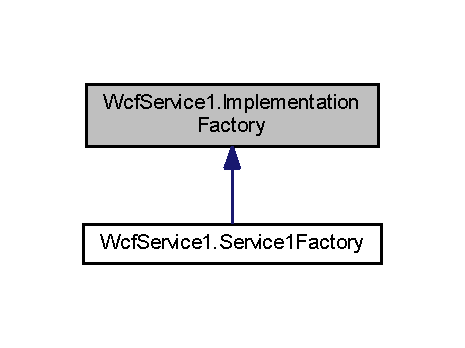
\includegraphics[width=223pt]{class_wcf_service1_1_1_implementation_factory__inherit__graph}
\end{center}
\end{figure}
\subsection*{Public Member Functions}
\begin{DoxyCompactItemize}
\item 
abstract \hyperlink{class_wcf_service1_1_1_service_class}{Service\+Class} \hyperlink{class_wcf_service1_1_1_implementation_factory_ae88b463f0c749ded38d5cbcf2c1dd7cb}{Get\+Implementation} ()
\end{DoxyCompactItemize}


\subsection{Detailed Description}
reference\+: \href{http://www.c-sharpcorner.com/article/factory-method-design-pattern-in-c-sharp/}{\tt http\+://www.\+c-\/sharpcorner.\+com/article/factory-\/method-\/design-\/pattern-\/in-\/c-\/sharp/} 



\subsection{Member Function Documentation}
\index{Wcf\+Service1\+::\+Implementation\+Factory@{Wcf\+Service1\+::\+Implementation\+Factory}!Get\+Implementation@{Get\+Implementation}}
\index{Get\+Implementation@{Get\+Implementation}!Wcf\+Service1\+::\+Implementation\+Factory@{Wcf\+Service1\+::\+Implementation\+Factory}}
\subsubsection[{\texorpdfstring{Get\+Implementation()}{GetImplementation()}}]{\setlength{\rightskip}{0pt plus 5cm}abstract {\bf Service\+Class} Wcf\+Service1.\+Implementation\+Factory.\+Get\+Implementation (
\begin{DoxyParamCaption}
{}
\end{DoxyParamCaption}
)\hspace{0.3cm}{\ttfamily [pure virtual]}}\hypertarget{class_wcf_service1_1_1_implementation_factory_ae88b463f0c749ded38d5cbcf2c1dd7cb}{}\label{class_wcf_service1_1_1_implementation_factory_ae88b463f0c749ded38d5cbcf2c1dd7cb}


Implemented in \hyperlink{class_wcf_service1_1_1_service1_factory_ae1204f90d6f8c4fcd4ad6b95cb6815b7}{Wcf\+Service1.\+Service1\+Factory}.



The documentation for this class was generated from the following file\+:\begin{DoxyCompactItemize}
\item 
C\+:/\+Users/user/source/repos/\+Hoermirzu/\+Listen\+To\+Me-\/master-\/89f0b49594deaade7bfad24dad062ff16eca36da/\+Wcf\+Service1/\hyperlink{_implementation_factory_8cs}{Implementation\+Factory.\+cs}\end{DoxyCompactItemize}

\hypertarget{interface_wcf_service1_1_1_i_service1}{}\section{Wcf\+Service1.\+I\+Service1 Interface Reference}
\label{interface_wcf_service1_1_1_i_service1}\index{Wcf\+Service1.\+I\+Service1@{Wcf\+Service1.\+I\+Service1}}


Inheritance diagram for Wcf\+Service1.\+I\+Service1\+:\nopagebreak
\begin{figure}[H]
\begin{center}
\leavevmode
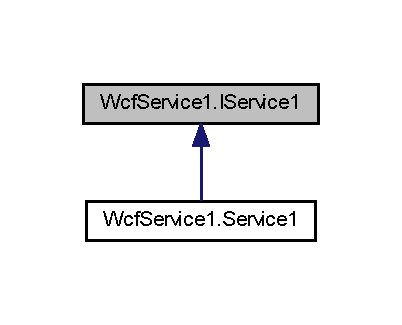
\includegraphics[width=193pt]{interface_wcf_service1_1_1_i_service1__inherit__graph}
\end{center}
\end{figure}
\subsection*{Public Member Functions}
\begin{DoxyCompactItemize}
\item 
string \hyperlink{interface_wcf_service1_1_1_i_service1_a22c297ac3e406ff48776942e47e6ba65}{Login} (string username, string password)
\item 
string \hyperlink{interface_wcf_service1_1_1_i_service1_ab0b52fb983ee4488ad7de5f03597d186}{Get\+Form} (string \+\_\+username, string \+\_\+password)
\item 
List$<$ string $>$ \hyperlink{interface_wcf_service1_1_1_i_service1_a81d8f9d0c98959c0db9856ef015ef71c}{Get\+Inputs} (string username, string password, string domain)
\item 
List$<$ string $>$ \hyperlink{interface_wcf_service1_1_1_i_service1_a62b4a23525791f79b35325acdc9c08c1}{Get\+Headings} (string username, string password, string domain)
\item 
List$<$ Section $>$ \hyperlink{interface_wcf_service1_1_1_i_service1_aa3f75be37b97eb1f0b0630cfabc2c51c}{Get\+All\+Elements} (string username, string password)
\item 
string \hyperlink{interface_wcf_service1_1_1_i_service1_a19ff6b5fd0d71880ef89413442e3eabe}{Read\+Jason\+From\+File} (string filename)
\item 
string \hyperlink{interface_wcf_service1_1_1_i_service1_a1baba4ded4ba686dc43912639339e1a0}{Get\+C\+S\+V\+Dropdown\+String} (string list\+\_\+id)
\item 
string \hyperlink{interface_wcf_service1_1_1_i_service1_aa4b0e92420addad7422e113b7b7161e2}{Serialize\+To\+Json} (string username, string password)
\item 
bool \hyperlink{interface_wcf_service1_1_1_i_service1_a40f5fb59f7eb2c10dc216bceb4fc366c}{Upload\+Section} (Section section)
\item 
Task$<$ string $>$ \hyperlink{interface_wcf_service1_1_1_i_service1_a1d49b0b16f20bd13e61cc1bb80aa7832}{Talk\+To\+The\+Bot\+Async} (string message)
\end{DoxyCompactItemize}


\subsection{Member Function Documentation}
\index{Wcf\+Service1\+::\+I\+Service1@{Wcf\+Service1\+::\+I\+Service1}!Get\+All\+Elements@{Get\+All\+Elements}}
\index{Get\+All\+Elements@{Get\+All\+Elements}!Wcf\+Service1\+::\+I\+Service1@{Wcf\+Service1\+::\+I\+Service1}}
\subsubsection[{\texorpdfstring{Get\+All\+Elements(string username, string password)}{GetAllElements(string username, string password)}}]{\setlength{\rightskip}{0pt plus 5cm}List$<$Section$>$ Wcf\+Service1.\+I\+Service1.\+Get\+All\+Elements (
\begin{DoxyParamCaption}
\item[{string}]{username, }
\item[{string}]{password}
\end{DoxyParamCaption}
)}\hypertarget{interface_wcf_service1_1_1_i_service1_aa3f75be37b97eb1f0b0630cfabc2c51c}{}\label{interface_wcf_service1_1_1_i_service1_aa3f75be37b97eb1f0b0630cfabc2c51c}


Implemented in \hyperlink{class_wcf_service1_1_1_service1_ab19a2f842aca61072732f113e7278ba6}{Wcf\+Service1.\+Service1}.

\index{Wcf\+Service1\+::\+I\+Service1@{Wcf\+Service1\+::\+I\+Service1}!Get\+C\+S\+V\+Dropdown\+String@{Get\+C\+S\+V\+Dropdown\+String}}
\index{Get\+C\+S\+V\+Dropdown\+String@{Get\+C\+S\+V\+Dropdown\+String}!Wcf\+Service1\+::\+I\+Service1@{Wcf\+Service1\+::\+I\+Service1}}
\subsubsection[{\texorpdfstring{Get\+C\+S\+V\+Dropdown\+String(string list\+\_\+id)}{GetCSVDropdownString(string list_id)}}]{\setlength{\rightskip}{0pt plus 5cm}string Wcf\+Service1.\+I\+Service1.\+Get\+C\+S\+V\+Dropdown\+String (
\begin{DoxyParamCaption}
\item[{string}]{list\+\_\+id}
\end{DoxyParamCaption}
)}\hypertarget{interface_wcf_service1_1_1_i_service1_a1baba4ded4ba686dc43912639339e1a0}{}\label{interface_wcf_service1_1_1_i_service1_a1baba4ded4ba686dc43912639339e1a0}


Implemented in \hyperlink{class_wcf_service1_1_1_service1_a3c0423e72454f64650ca89e43aa30955}{Wcf\+Service1.\+Service1}.

\index{Wcf\+Service1\+::\+I\+Service1@{Wcf\+Service1\+::\+I\+Service1}!Get\+Form@{Get\+Form}}
\index{Get\+Form@{Get\+Form}!Wcf\+Service1\+::\+I\+Service1@{Wcf\+Service1\+::\+I\+Service1}}
\subsubsection[{\texorpdfstring{Get\+Form(string \+\_\+username, string \+\_\+password)}{GetForm(string _username, string _password)}}]{\setlength{\rightskip}{0pt plus 5cm}string Wcf\+Service1.\+I\+Service1.\+Get\+Form (
\begin{DoxyParamCaption}
\item[{string}]{\+\_\+username, }
\item[{string}]{\+\_\+password}
\end{DoxyParamCaption}
)}\hypertarget{interface_wcf_service1_1_1_i_service1_ab0b52fb983ee4488ad7de5f03597d186}{}\label{interface_wcf_service1_1_1_i_service1_ab0b52fb983ee4488ad7de5f03597d186}


Implemented in \hyperlink{class_wcf_service1_1_1_service1_a13eccecdb2a4a36fbbbd96f2ff07f880}{Wcf\+Service1.\+Service1}.

\index{Wcf\+Service1\+::\+I\+Service1@{Wcf\+Service1\+::\+I\+Service1}!Get\+Headings@{Get\+Headings}}
\index{Get\+Headings@{Get\+Headings}!Wcf\+Service1\+::\+I\+Service1@{Wcf\+Service1\+::\+I\+Service1}}
\subsubsection[{\texorpdfstring{Get\+Headings(string username, string password, string domain)}{GetHeadings(string username, string password, string domain)}}]{\setlength{\rightskip}{0pt plus 5cm}List$<$string$>$ Wcf\+Service1.\+I\+Service1.\+Get\+Headings (
\begin{DoxyParamCaption}
\item[{string}]{username, }
\item[{string}]{password, }
\item[{string}]{domain}
\end{DoxyParamCaption}
)}\hypertarget{interface_wcf_service1_1_1_i_service1_a62b4a23525791f79b35325acdc9c08c1}{}\label{interface_wcf_service1_1_1_i_service1_a62b4a23525791f79b35325acdc9c08c1}


Implemented in \hyperlink{class_wcf_service1_1_1_service1_a9a93a18651e7fd879d8166bd70abdbfe}{Wcf\+Service1.\+Service1}.

\index{Wcf\+Service1\+::\+I\+Service1@{Wcf\+Service1\+::\+I\+Service1}!Get\+Inputs@{Get\+Inputs}}
\index{Get\+Inputs@{Get\+Inputs}!Wcf\+Service1\+::\+I\+Service1@{Wcf\+Service1\+::\+I\+Service1}}
\subsubsection[{\texorpdfstring{Get\+Inputs(string username, string password, string domain)}{GetInputs(string username, string password, string domain)}}]{\setlength{\rightskip}{0pt plus 5cm}List$<$string$>$ Wcf\+Service1.\+I\+Service1.\+Get\+Inputs (
\begin{DoxyParamCaption}
\item[{string}]{username, }
\item[{string}]{password, }
\item[{string}]{domain}
\end{DoxyParamCaption}
)}\hypertarget{interface_wcf_service1_1_1_i_service1_a81d8f9d0c98959c0db9856ef015ef71c}{}\label{interface_wcf_service1_1_1_i_service1_a81d8f9d0c98959c0db9856ef015ef71c}


Implemented in \hyperlink{class_wcf_service1_1_1_service1_ad9115f054786f723b3bcb4f3f62457ba}{Wcf\+Service1.\+Service1}.

\index{Wcf\+Service1\+::\+I\+Service1@{Wcf\+Service1\+::\+I\+Service1}!Login@{Login}}
\index{Login@{Login}!Wcf\+Service1\+::\+I\+Service1@{Wcf\+Service1\+::\+I\+Service1}}
\subsubsection[{\texorpdfstring{Login(string username, string password)}{Login(string username, string password)}}]{\setlength{\rightskip}{0pt plus 5cm}string Wcf\+Service1.\+I\+Service1.\+Login (
\begin{DoxyParamCaption}
\item[{string}]{username, }
\item[{string}]{password}
\end{DoxyParamCaption}
)}\hypertarget{interface_wcf_service1_1_1_i_service1_a22c297ac3e406ff48776942e47e6ba65}{}\label{interface_wcf_service1_1_1_i_service1_a22c297ac3e406ff48776942e47e6ba65}


Implemented in \hyperlink{class_wcf_service1_1_1_service1_a451391230a00d5f6ea6aafd54aad1a12}{Wcf\+Service1.\+Service1}.

\index{Wcf\+Service1\+::\+I\+Service1@{Wcf\+Service1\+::\+I\+Service1}!Read\+Jason\+From\+File@{Read\+Jason\+From\+File}}
\index{Read\+Jason\+From\+File@{Read\+Jason\+From\+File}!Wcf\+Service1\+::\+I\+Service1@{Wcf\+Service1\+::\+I\+Service1}}
\subsubsection[{\texorpdfstring{Read\+Jason\+From\+File(string filename)}{ReadJasonFromFile(string filename)}}]{\setlength{\rightskip}{0pt plus 5cm}string Wcf\+Service1.\+I\+Service1.\+Read\+Jason\+From\+File (
\begin{DoxyParamCaption}
\item[{string}]{filename}
\end{DoxyParamCaption}
)}\hypertarget{interface_wcf_service1_1_1_i_service1_a19ff6b5fd0d71880ef89413442e3eabe}{}\label{interface_wcf_service1_1_1_i_service1_a19ff6b5fd0d71880ef89413442e3eabe}


Implemented in \hyperlink{class_wcf_service1_1_1_service1_a1efce216795958b0c4e3f176665027fe}{Wcf\+Service1.\+Service1}.

\index{Wcf\+Service1\+::\+I\+Service1@{Wcf\+Service1\+::\+I\+Service1}!Serialize\+To\+Json@{Serialize\+To\+Json}}
\index{Serialize\+To\+Json@{Serialize\+To\+Json}!Wcf\+Service1\+::\+I\+Service1@{Wcf\+Service1\+::\+I\+Service1}}
\subsubsection[{\texorpdfstring{Serialize\+To\+Json(string username, string password)}{SerializeToJson(string username, string password)}}]{\setlength{\rightskip}{0pt plus 5cm}string Wcf\+Service1.\+I\+Service1.\+Serialize\+To\+Json (
\begin{DoxyParamCaption}
\item[{string}]{username, }
\item[{string}]{password}
\end{DoxyParamCaption}
)}\hypertarget{interface_wcf_service1_1_1_i_service1_aa4b0e92420addad7422e113b7b7161e2}{}\label{interface_wcf_service1_1_1_i_service1_aa4b0e92420addad7422e113b7b7161e2}


Implemented in \hyperlink{class_wcf_service1_1_1_service1_abc900a9de8f8aa5a126f1eef3353b154}{Wcf\+Service1.\+Service1}.

\index{Wcf\+Service1\+::\+I\+Service1@{Wcf\+Service1\+::\+I\+Service1}!Talk\+To\+The\+Bot\+Async@{Talk\+To\+The\+Bot\+Async}}
\index{Talk\+To\+The\+Bot\+Async@{Talk\+To\+The\+Bot\+Async}!Wcf\+Service1\+::\+I\+Service1@{Wcf\+Service1\+::\+I\+Service1}}
\subsubsection[{\texorpdfstring{Talk\+To\+The\+Bot\+Async(string message)}{TalkToTheBotAsync(string message)}}]{\setlength{\rightskip}{0pt plus 5cm}Task$<$string$>$ Wcf\+Service1.\+I\+Service1.\+Talk\+To\+The\+Bot\+Async (
\begin{DoxyParamCaption}
\item[{string}]{message}
\end{DoxyParamCaption}
)}\hypertarget{interface_wcf_service1_1_1_i_service1_a1d49b0b16f20bd13e61cc1bb80aa7832}{}\label{interface_wcf_service1_1_1_i_service1_a1d49b0b16f20bd13e61cc1bb80aa7832}


Implemented in \hyperlink{class_wcf_service1_1_1_service1_a3073c327f0dae7f2a6324341bbefcaf8}{Wcf\+Service1.\+Service1}.

\index{Wcf\+Service1\+::\+I\+Service1@{Wcf\+Service1\+::\+I\+Service1}!Upload\+Section@{Upload\+Section}}
\index{Upload\+Section@{Upload\+Section}!Wcf\+Service1\+::\+I\+Service1@{Wcf\+Service1\+::\+I\+Service1}}
\subsubsection[{\texorpdfstring{Upload\+Section(\+Section section)}{UploadSection(Section section)}}]{\setlength{\rightskip}{0pt plus 5cm}bool Wcf\+Service1.\+I\+Service1.\+Upload\+Section (
\begin{DoxyParamCaption}
\item[{Section}]{section}
\end{DoxyParamCaption}
)}\hypertarget{interface_wcf_service1_1_1_i_service1_a40f5fb59f7eb2c10dc216bceb4fc366c}{}\label{interface_wcf_service1_1_1_i_service1_a40f5fb59f7eb2c10dc216bceb4fc366c}


Implemented in \hyperlink{class_wcf_service1_1_1_service1_a4ba31cd1a202c84fac4d03461d8f4361}{Wcf\+Service1.\+Service1}.



The documentation for this interface was generated from the following file\+:\begin{DoxyCompactItemize}
\item 
C\+:/\+Users/user/source/repos/\+Hoermirzu/\+Listen\+To\+Me-\/master-\/89f0b49594deaade7bfad24dad062ff16eca36da/\+Wcf\+Service1/\hyperlink{_i_service1_8cs}{I\+Service1.\+cs}\end{DoxyCompactItemize}

\hypertarget{class_wcf_service1_1_1_service1}{}\section{Wcf\+Service1.\+Service1 Class Reference}
\label{class_wcf_service1_1_1_service1}\index{Wcf\+Service1.\+Service1@{Wcf\+Service1.\+Service1}}


the class implements the webservice parsing the form. ther is a debug and no-\/debug mode. If Debug is true, the form is build from a json text fine. If not it\textquotesingle{}s delivered fróm a Selenium Browser \hyperlink{class_wcf_service1_1_1_website_crawler}{Website\+Crawler}  




Inheritance diagram for Wcf\+Service1.\+Service1\+:\nopagebreak
\begin{figure}[H]
\begin{center}
\leavevmode
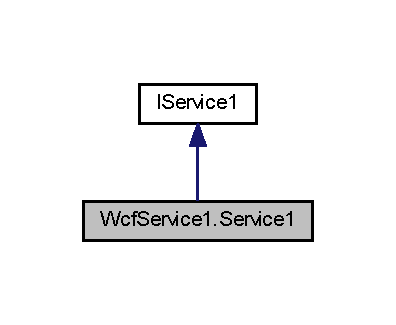
\includegraphics[width=190pt]{class_wcf_service1_1_1_service1__inherit__graph}
\end{center}
\end{figure}


Collaboration diagram for Wcf\+Service1.\+Service1\+:\nopagebreak
\begin{figure}[H]
\begin{center}
\leavevmode
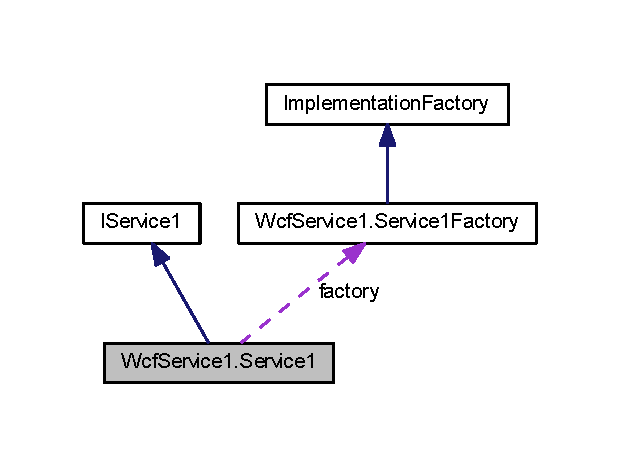
\includegraphics[width=298pt]{class_wcf_service1_1_1_service1__coll__graph}
\end{center}
\end{figure}
\subsection*{Public Member Functions}
\begin{DoxyCompactItemize}
\item 
string \hyperlink{class_wcf_service1_1_1_service1_a451391230a00d5f6ea6aafd54aad1a12}{Login} (string \+\_\+user\+Name, string \+\_\+password)
\begin{DoxyCompactList}\small\item\em real login to the web form \end{DoxyCompactList}\item 
string \hyperlink{class_wcf_service1_1_1_service1_a13eccecdb2a4a36fbbbd96f2ff07f880}{Get\+Form} (string \+\_\+username, string \+\_\+password)
\begin{DoxyCompactList}\small\item\em is telling the headless browser to navigate to a specific domain in order to login and view the form \end{DoxyCompactList}\item 
List$<$ string $>$ \hyperlink{class_wcf_service1_1_1_service1_ad9115f054786f723b3bcb4f3f62457ba}{Get\+Inputs} (string username, string password, string domain)
\begin{DoxyCompactList}\small\item\em returns a list of all labels on the web form. Those can then be translated into text\+Boxes by the App \end{DoxyCompactList}\item 
List$<$ string $>$ \hyperlink{class_wcf_service1_1_1_service1_a9a93a18651e7fd879d8166bd70abdbfe}{Get\+Headings} (string username, string password, string domain)
\begin{DoxyCompactList}\small\item\em Is returning headings slightly modified, cuts the number from the heading e.\+g \end{DoxyCompactList}\item 
List$<$ Section $>$ \hyperlink{class_wcf_service1_1_1_service1_ab19a2f842aca61072732f113e7278ba6}{Get\+All\+Elements} (string username, string password)
\begin{DoxyCompactList}\small\item\em parses the website form and returns a json string simulating radio buttons, check-\/boxec, input fields, headings, dopdown lists, date pickers and labels. This is specialized for these control types and other types will not be recognized this is not working correctly. In the inputs and headings region old values are kept don\textquotesingle{}t use this in debug mude, returns only partial output \end{DoxyCompactList}\item 
string \hyperlink{class_wcf_service1_1_1_service1_abc900a9de8f8aa5a126f1eef3353b154}{Serialize\+To\+Json} (string username, string password)
\begin{DoxyCompactList}\small\item\em serializes a Dictionary to a json string with indented formatting not needed with current factory pattern \end{DoxyCompactList}\item 
string \hyperlink{class_wcf_service1_1_1_service1_a1efce216795958b0c4e3f176665027fe}{Read\+Jason\+From\+File} (string filename)
\begin{DoxyCompactList}\small\item\em reads the json sections from a file. This is used in debugging if the web form is not available \end{DoxyCompactList}\item 
string \hyperlink{class_wcf_service1_1_1_service1_a3c0423e72454f64650ca89e43aa30955}{Get\+C\+S\+V\+Dropdown\+String} (string list\+\_\+id)
\item 
Task$<$ string $>$ \hyperlink{class_wcf_service1_1_1_service1_a3073c327f0dae7f2a6324341bbefcaf8}{Talk\+To\+The\+Bot\+Async} (string message)
\item 
bool \hyperlink{class_wcf_service1_1_1_service1_a4ba31cd1a202c84fac4d03461d8f4361}{Upload\+Section} (Section section)
\end{DoxyCompactItemize}
\subsection*{Private Member Functions}
\begin{DoxyCompactItemize}
\item 
string \hyperlink{class_wcf_service1_1_1_service1_a499bdb13585860a3ac6042e511b267ef}{convert\+H\+T\+M\+L\+Doc\+To\+X\+M\+L\+Doc} (Html\+Document doc)
\begin{DoxyCompactList}\small\item\em could help at converting the html to xml. xml was originally used in the formstore. \end{DoxyCompactList}\end{DoxyCompactItemize}
\subsection*{Private Attributes}
\begin{DoxyCompactItemize}
\item 
\hyperlink{class_wcf_service1_1_1_service1_factory}{Service1\+Factory} \hyperlink{class_wcf_service1_1_1_service1_a7ff9458393176c80aa7d4365896de3b0}{factory} = new \hyperlink{class_wcf_service1_1_1_service1_factory}{Service1\+Factory}(true)
\begin{DoxyCompactList}\small\item\em Factory returning the Mock Document(param true) or the real Document(param false) \end{DoxyCompactList}\end{DoxyCompactItemize}


\subsection{Detailed Description}
the class implements the webservice parsing the form. ther is a debug and no-\/debug mode. If Debug is true, the form is build from a json text fine. If not it\textquotesingle{}s delivered fróm a Selenium Browser \hyperlink{class_wcf_service1_1_1_website_crawler}{Website\+Crawler} 



\subsection{Member Function Documentation}
\index{Wcf\+Service1\+::\+Service1@{Wcf\+Service1\+::\+Service1}!convert\+H\+T\+M\+L\+Doc\+To\+X\+M\+L\+Doc@{convert\+H\+T\+M\+L\+Doc\+To\+X\+M\+L\+Doc}}
\index{convert\+H\+T\+M\+L\+Doc\+To\+X\+M\+L\+Doc@{convert\+H\+T\+M\+L\+Doc\+To\+X\+M\+L\+Doc}!Wcf\+Service1\+::\+Service1@{Wcf\+Service1\+::\+Service1}}
\subsubsection[{\texorpdfstring{convert\+H\+T\+M\+L\+Doc\+To\+X\+M\+L\+Doc(\+Html\+Document doc)}{convertHTMLDocToXMLDoc(HtmlDocument doc)}}]{\setlength{\rightskip}{0pt plus 5cm}string Wcf\+Service1.\+Service1.\+convert\+H\+T\+M\+L\+Doc\+To\+X\+M\+L\+Doc (
\begin{DoxyParamCaption}
\item[{Html\+Document}]{doc}
\end{DoxyParamCaption}
)\hspace{0.3cm}{\ttfamily [private]}}\hypertarget{class_wcf_service1_1_1_service1_a499bdb13585860a3ac6042e511b267ef}{}\label{class_wcf_service1_1_1_service1_a499bdb13585860a3ac6042e511b267ef}


could help at converting the html to xml. xml was originally used in the formstore. 


\begin{DoxyParams}{Parameters}
{\em doc} & the html document to be converted\\
\hline
\end{DoxyParams}
\begin{DoxyReturn}{Returns}

\end{DoxyReturn}
\index{Wcf\+Service1\+::\+Service1@{Wcf\+Service1\+::\+Service1}!Get\+All\+Elements@{Get\+All\+Elements}}
\index{Get\+All\+Elements@{Get\+All\+Elements}!Wcf\+Service1\+::\+Service1@{Wcf\+Service1\+::\+Service1}}
\subsubsection[{\texorpdfstring{Get\+All\+Elements(string username, string password)}{GetAllElements(string username, string password)}}]{\setlength{\rightskip}{0pt plus 5cm}List$<$Section$>$ Wcf\+Service1.\+Service1.\+Get\+All\+Elements (
\begin{DoxyParamCaption}
\item[{string}]{username, }
\item[{string}]{password}
\end{DoxyParamCaption}
)}\hypertarget{class_wcf_service1_1_1_service1_ab19a2f842aca61072732f113e7278ba6}{}\label{class_wcf_service1_1_1_service1_ab19a2f842aca61072732f113e7278ba6}


parses the website form and returns a json string simulating radio buttons, check-\/boxec, input fields, headings, dopdown lists, date pickers and labels. This is specialized for these control types and other types will not be recognized this is not working correctly. In the inputs and headings region old values are kept don\textquotesingle{}t use this in debug mude, returns only partial output 


\begin{DoxyParams}{Parameters}
{\em username} & \\
\hline
{\em password} & \\
\hline
{\em is\+Debug} & \\
\hline
\end{DoxyParams}
\begin{DoxyReturn}{Returns}
returns Json string containing structure for a Section
\end{DoxyReturn}


Implements \hyperlink{interface_wcf_service1_1_1_i_service1_aa3f75be37b97eb1f0b0630cfabc2c51c}{Wcf\+Service1.\+I\+Service1}.



Here is the call graph for this function\+:\nopagebreak
\begin{figure}[H]
\begin{center}
\leavevmode
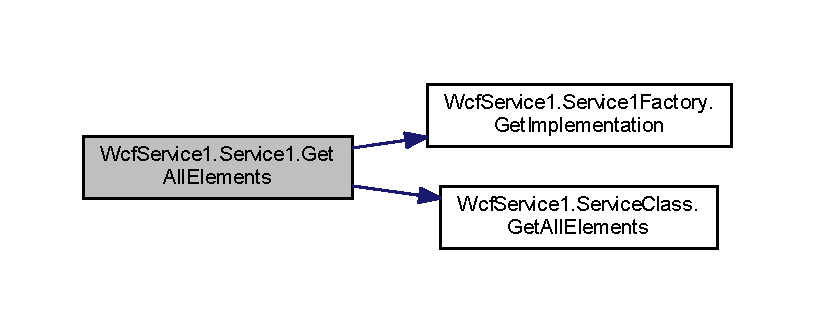
\includegraphics[width=350pt]{class_wcf_service1_1_1_service1_ab19a2f842aca61072732f113e7278ba6_cgraph}
\end{center}
\end{figure}




Here is the caller graph for this function\+:\nopagebreak
\begin{figure}[H]
\begin{center}
\leavevmode
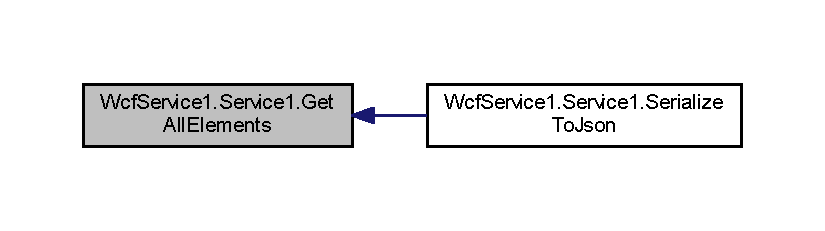
\includegraphics[width=350pt]{class_wcf_service1_1_1_service1_ab19a2f842aca61072732f113e7278ba6_icgraph}
\end{center}
\end{figure}


\index{Wcf\+Service1\+::\+Service1@{Wcf\+Service1\+::\+Service1}!Get\+C\+S\+V\+Dropdown\+String@{Get\+C\+S\+V\+Dropdown\+String}}
\index{Get\+C\+S\+V\+Dropdown\+String@{Get\+C\+S\+V\+Dropdown\+String}!Wcf\+Service1\+::\+Service1@{Wcf\+Service1\+::\+Service1}}
\subsubsection[{\texorpdfstring{Get\+C\+S\+V\+Dropdown\+String(string list\+\_\+id)}{GetCSVDropdownString(string list_id)}}]{\setlength{\rightskip}{0pt plus 5cm}string Wcf\+Service1.\+Service1.\+Get\+C\+S\+V\+Dropdown\+String (
\begin{DoxyParamCaption}
\item[{string}]{list\+\_\+id}
\end{DoxyParamCaption}
)}\hypertarget{class_wcf_service1_1_1_service1_a3c0423e72454f64650ca89e43aa30955}{}\label{class_wcf_service1_1_1_service1_a3c0423e72454f64650ca89e43aa30955}


Implements \hyperlink{interface_wcf_service1_1_1_i_service1_a1baba4ded4ba686dc43912639339e1a0}{Wcf\+Service1.\+I\+Service1}.



Here is the call graph for this function\+:\nopagebreak
\begin{figure}[H]
\begin{center}
\leavevmode
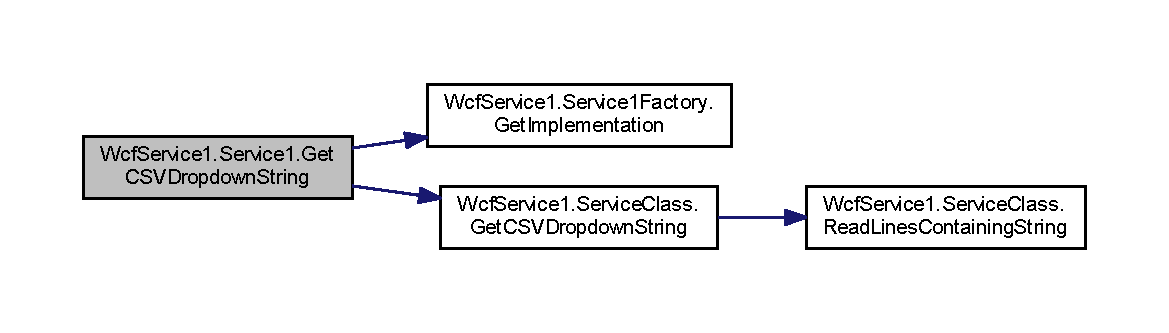
\includegraphics[width=350pt]{class_wcf_service1_1_1_service1_a3c0423e72454f64650ca89e43aa30955_cgraph}
\end{center}
\end{figure}


\index{Wcf\+Service1\+::\+Service1@{Wcf\+Service1\+::\+Service1}!Get\+Form@{Get\+Form}}
\index{Get\+Form@{Get\+Form}!Wcf\+Service1\+::\+Service1@{Wcf\+Service1\+::\+Service1}}
\subsubsection[{\texorpdfstring{Get\+Form(string \+\_\+username, string \+\_\+password)}{GetForm(string _username, string _password)}}]{\setlength{\rightskip}{0pt plus 5cm}string Wcf\+Service1.\+Service1.\+Get\+Form (
\begin{DoxyParamCaption}
\item[{string}]{\+\_\+username, }
\item[{string}]{\+\_\+password}
\end{DoxyParamCaption}
)}\hypertarget{class_wcf_service1_1_1_service1_a13eccecdb2a4a36fbbbd96f2ff07f880}{}\label{class_wcf_service1_1_1_service1_a13eccecdb2a4a36fbbbd96f2ff07f880}


is telling the headless browser to navigate to a specific domain in order to login and view the form 


\begin{DoxyParams}{Parameters}
{\em \+\_\+username} & \\
\hline
{\em \+\_\+password} & \\
\hline
\end{DoxyParams}
\begin{DoxyReturn}{Returns}

\end{DoxyReturn}


Implements \hyperlink{interface_wcf_service1_1_1_i_service1_ab0b52fb983ee4488ad7de5f03597d186}{Wcf\+Service1.\+I\+Service1}.



Here is the call graph for this function\+:\nopagebreak
\begin{figure}[H]
\begin{center}
\leavevmode
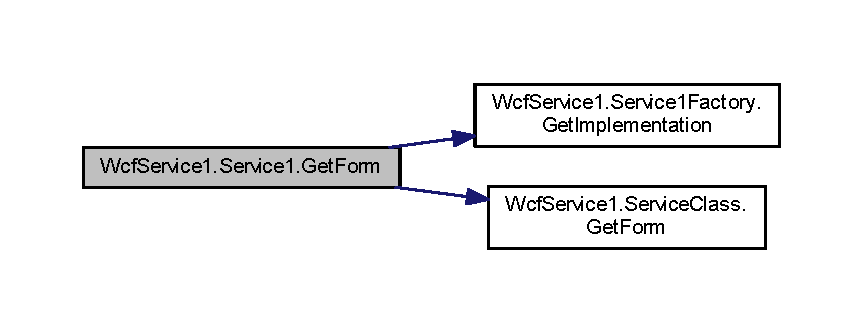
\includegraphics[width=350pt]{class_wcf_service1_1_1_service1_a13eccecdb2a4a36fbbbd96f2ff07f880_cgraph}
\end{center}
\end{figure}


\index{Wcf\+Service1\+::\+Service1@{Wcf\+Service1\+::\+Service1}!Get\+Headings@{Get\+Headings}}
\index{Get\+Headings@{Get\+Headings}!Wcf\+Service1\+::\+Service1@{Wcf\+Service1\+::\+Service1}}
\subsubsection[{\texorpdfstring{Get\+Headings(string username, string password, string domain)}{GetHeadings(string username, string password, string domain)}}]{\setlength{\rightskip}{0pt plus 5cm}List$<$string$>$ Wcf\+Service1.\+Service1.\+Get\+Headings (
\begin{DoxyParamCaption}
\item[{string}]{username, }
\item[{string}]{password, }
\item[{string}]{domain}
\end{DoxyParamCaption}
)}\hypertarget{class_wcf_service1_1_1_service1_a9a93a18651e7fd879d8166bd70abdbfe}{}\label{class_wcf_service1_1_1_service1_a9a93a18651e7fd879d8166bd70abdbfe}


Is returning headings slightly modified, cuts the number from the heading e.\+g 


\begin{DoxyParams}{Parameters}
{\em username} & \\
\hline
{\em password} & \\
\hline
{\em domain} & \\
\hline
\end{DoxyParams}
\begin{DoxyReturn}{Returns}

\end{DoxyReturn}


Implements \hyperlink{interface_wcf_service1_1_1_i_service1_a62b4a23525791f79b35325acdc9c08c1}{Wcf\+Service1.\+I\+Service1}.



Here is the call graph for this function\+:\nopagebreak
\begin{figure}[H]
\begin{center}
\leavevmode
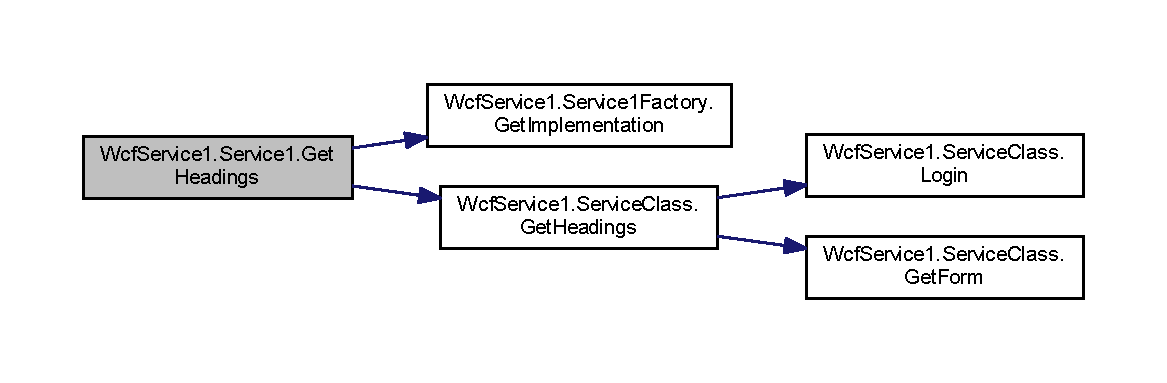
\includegraphics[width=350pt]{class_wcf_service1_1_1_service1_a9a93a18651e7fd879d8166bd70abdbfe_cgraph}
\end{center}
\end{figure}


\index{Wcf\+Service1\+::\+Service1@{Wcf\+Service1\+::\+Service1}!Get\+Inputs@{Get\+Inputs}}
\index{Get\+Inputs@{Get\+Inputs}!Wcf\+Service1\+::\+Service1@{Wcf\+Service1\+::\+Service1}}
\subsubsection[{\texorpdfstring{Get\+Inputs(string username, string password, string domain)}{GetInputs(string username, string password, string domain)}}]{\setlength{\rightskip}{0pt plus 5cm}List$<$string$>$ Wcf\+Service1.\+Service1.\+Get\+Inputs (
\begin{DoxyParamCaption}
\item[{string}]{username, }
\item[{string}]{password, }
\item[{string}]{domain}
\end{DoxyParamCaption}
)}\hypertarget{class_wcf_service1_1_1_service1_ad9115f054786f723b3bcb4f3f62457ba}{}\label{class_wcf_service1_1_1_service1_ad9115f054786f723b3bcb4f3f62457ba}


returns a list of all labels on the web form. Those can then be translated into text\+Boxes by the App 


\begin{DoxyParams}{Parameters}
{\em username} & \\
\hline
{\em password} & \\
\hline
{\em domain} & \\
\hline
\end{DoxyParams}
\begin{DoxyReturn}{Returns}

\end{DoxyReturn}


Implements \hyperlink{interface_wcf_service1_1_1_i_service1_a81d8f9d0c98959c0db9856ef015ef71c}{Wcf\+Service1.\+I\+Service1}.



Here is the call graph for this function\+:\nopagebreak
\begin{figure}[H]
\begin{center}
\leavevmode
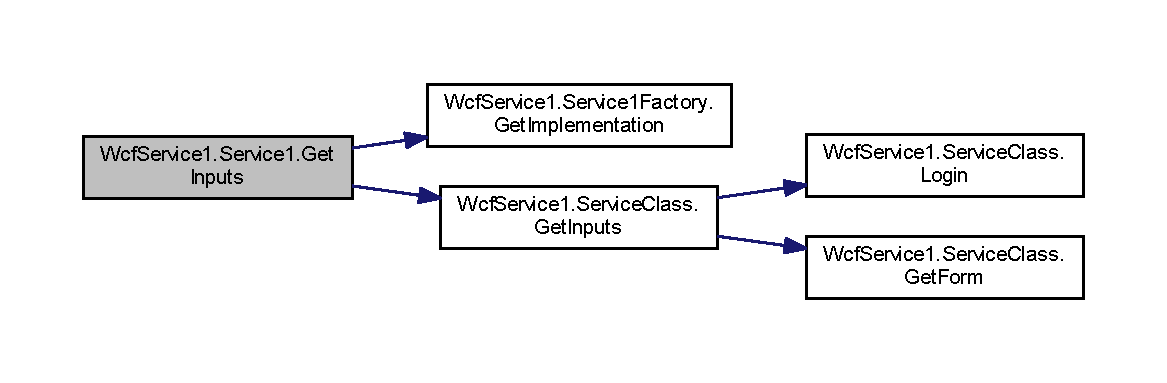
\includegraphics[width=350pt]{class_wcf_service1_1_1_service1_ad9115f054786f723b3bcb4f3f62457ba_cgraph}
\end{center}
\end{figure}


\index{Wcf\+Service1\+::\+Service1@{Wcf\+Service1\+::\+Service1}!Login@{Login}}
\index{Login@{Login}!Wcf\+Service1\+::\+Service1@{Wcf\+Service1\+::\+Service1}}
\subsubsection[{\texorpdfstring{Login(string \+\_\+user\+Name, string \+\_\+password)}{Login(string _userName, string _password)}}]{\setlength{\rightskip}{0pt plus 5cm}string Wcf\+Service1.\+Service1.\+Login (
\begin{DoxyParamCaption}
\item[{string}]{\+\_\+user\+Name, }
\item[{string}]{\+\_\+password}
\end{DoxyParamCaption}
)}\hypertarget{class_wcf_service1_1_1_service1_a451391230a00d5f6ea6aafd54aad1a12}{}\label{class_wcf_service1_1_1_service1_a451391230a00d5f6ea6aafd54aad1a12}


real login to the web form 


\begin{DoxyParams}{Parameters}
{\em \+\_\+user\+Name} & \\
\hline
{\em \+\_\+password} & \\
\hline
\end{DoxyParams}
\begin{DoxyReturn}{Returns}

\end{DoxyReturn}


Implements \hyperlink{interface_wcf_service1_1_1_i_service1_a22c297ac3e406ff48776942e47e6ba65}{Wcf\+Service1.\+I\+Service1}.



Here is the call graph for this function\+:\nopagebreak
\begin{figure}[H]
\begin{center}
\leavevmode
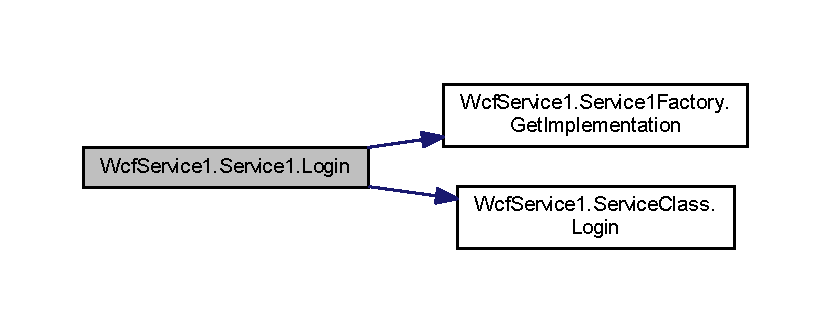
\includegraphics[width=350pt]{class_wcf_service1_1_1_service1_a451391230a00d5f6ea6aafd54aad1a12_cgraph}
\end{center}
\end{figure}


\index{Wcf\+Service1\+::\+Service1@{Wcf\+Service1\+::\+Service1}!Read\+Jason\+From\+File@{Read\+Jason\+From\+File}}
\index{Read\+Jason\+From\+File@{Read\+Jason\+From\+File}!Wcf\+Service1\+::\+Service1@{Wcf\+Service1\+::\+Service1}}
\subsubsection[{\texorpdfstring{Read\+Jason\+From\+File(string filename)}{ReadJasonFromFile(string filename)}}]{\setlength{\rightskip}{0pt plus 5cm}string Wcf\+Service1.\+Service1.\+Read\+Jason\+From\+File (
\begin{DoxyParamCaption}
\item[{string}]{filename}
\end{DoxyParamCaption}
)}\hypertarget{class_wcf_service1_1_1_service1_a1efce216795958b0c4e3f176665027fe}{}\label{class_wcf_service1_1_1_service1_a1efce216795958b0c4e3f176665027fe}


reads the json sections from a file. This is used in debugging if the web form is not available 

\begin{DoxyReturn}{Returns}

\end{DoxyReturn}


Implements \hyperlink{interface_wcf_service1_1_1_i_service1_a19ff6b5fd0d71880ef89413442e3eabe}{Wcf\+Service1.\+I\+Service1}.



Here is the call graph for this function\+:\nopagebreak
\begin{figure}[H]
\begin{center}
\leavevmode
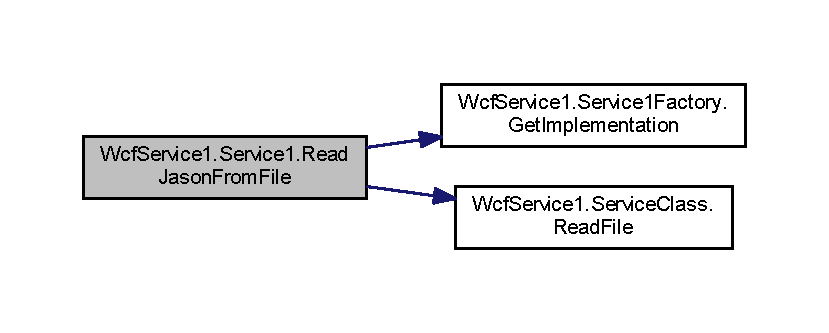
\includegraphics[width=350pt]{class_wcf_service1_1_1_service1_a1efce216795958b0c4e3f176665027fe_cgraph}
\end{center}
\end{figure}


\index{Wcf\+Service1\+::\+Service1@{Wcf\+Service1\+::\+Service1}!Serialize\+To\+Json@{Serialize\+To\+Json}}
\index{Serialize\+To\+Json@{Serialize\+To\+Json}!Wcf\+Service1\+::\+Service1@{Wcf\+Service1\+::\+Service1}}
\subsubsection[{\texorpdfstring{Serialize\+To\+Json(string username, string password)}{SerializeToJson(string username, string password)}}]{\setlength{\rightskip}{0pt plus 5cm}string Wcf\+Service1.\+Service1.\+Serialize\+To\+Json (
\begin{DoxyParamCaption}
\item[{string}]{username, }
\item[{string}]{password}
\end{DoxyParamCaption}
)}\hypertarget{class_wcf_service1_1_1_service1_abc900a9de8f8aa5a126f1eef3353b154}{}\label{class_wcf_service1_1_1_service1_abc900a9de8f8aa5a126f1eef3353b154}


serializes a Dictionary to a json string with indented formatting not needed with current factory pattern 


\begin{DoxyParams}{Parameters}
{\em json\+Dictionary} & the\\
\hline
\end{DoxyParams}
\begin{DoxyReturn}{Returns}

\end{DoxyReturn}


Implements \hyperlink{interface_wcf_service1_1_1_i_service1_aa4b0e92420addad7422e113b7b7161e2}{Wcf\+Service1.\+I\+Service1}.



Here is the call graph for this function\+:\nopagebreak
\begin{figure}[H]
\begin{center}
\leavevmode
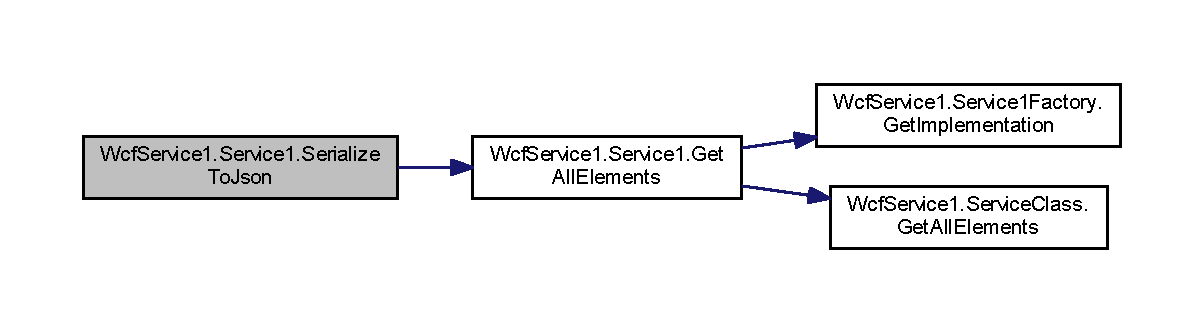
\includegraphics[width=350pt]{class_wcf_service1_1_1_service1_abc900a9de8f8aa5a126f1eef3353b154_cgraph}
\end{center}
\end{figure}


\index{Wcf\+Service1\+::\+Service1@{Wcf\+Service1\+::\+Service1}!Talk\+To\+The\+Bot\+Async@{Talk\+To\+The\+Bot\+Async}}
\index{Talk\+To\+The\+Bot\+Async@{Talk\+To\+The\+Bot\+Async}!Wcf\+Service1\+::\+Service1@{Wcf\+Service1\+::\+Service1}}
\subsubsection[{\texorpdfstring{Talk\+To\+The\+Bot\+Async(string message)}{TalkToTheBotAsync(string message)}}]{\setlength{\rightskip}{0pt plus 5cm}Task$<$string$>$ Wcf\+Service1.\+Service1.\+Talk\+To\+The\+Bot\+Async (
\begin{DoxyParamCaption}
\item[{string}]{message}
\end{DoxyParamCaption}
)}\hypertarget{class_wcf_service1_1_1_service1_a3073c327f0dae7f2a6324341bbefcaf8}{}\label{class_wcf_service1_1_1_service1_a3073c327f0dae7f2a6324341bbefcaf8}


Implements \hyperlink{interface_wcf_service1_1_1_i_service1_a1d49b0b16f20bd13e61cc1bb80aa7832}{Wcf\+Service1.\+I\+Service1}.



Here is the call graph for this function\+:\nopagebreak
\begin{figure}[H]
\begin{center}
\leavevmode
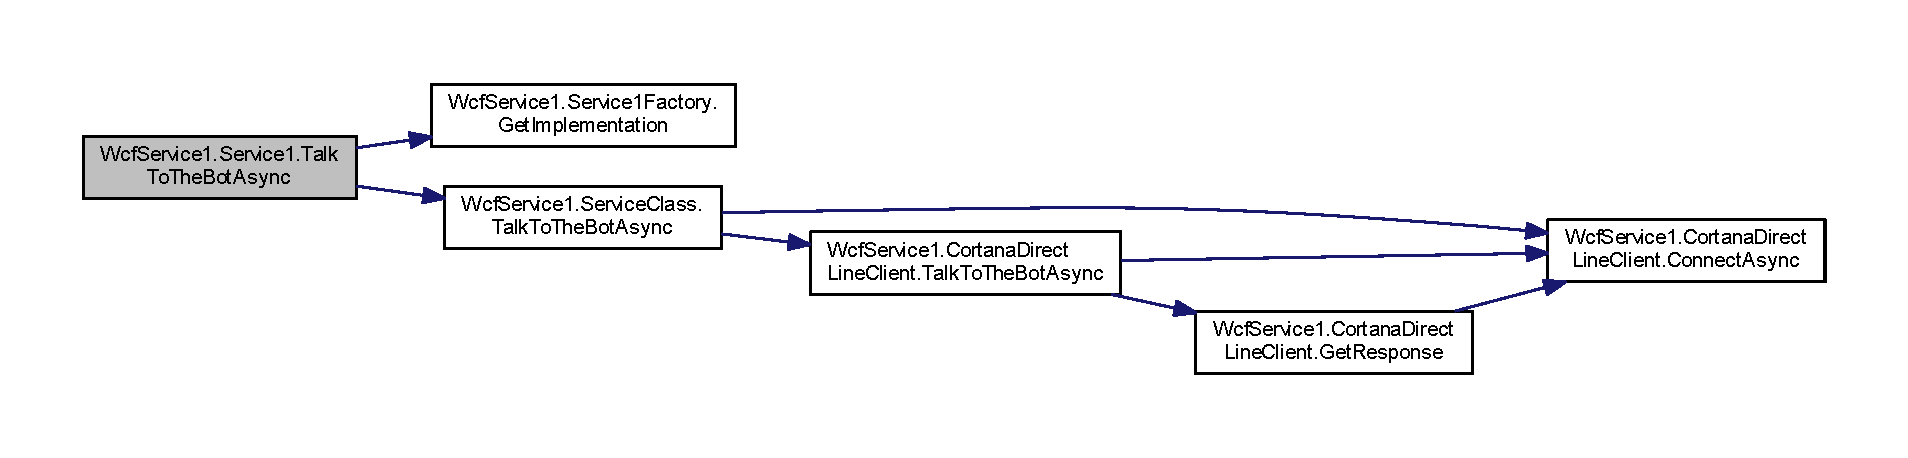
\includegraphics[width=350pt]{class_wcf_service1_1_1_service1_a3073c327f0dae7f2a6324341bbefcaf8_cgraph}
\end{center}
\end{figure}


\index{Wcf\+Service1\+::\+Service1@{Wcf\+Service1\+::\+Service1}!Upload\+Section@{Upload\+Section}}
\index{Upload\+Section@{Upload\+Section}!Wcf\+Service1\+::\+Service1@{Wcf\+Service1\+::\+Service1}}
\subsubsection[{\texorpdfstring{Upload\+Section(\+Section section)}{UploadSection(Section section)}}]{\setlength{\rightskip}{0pt plus 5cm}bool Wcf\+Service1.\+Service1.\+Upload\+Section (
\begin{DoxyParamCaption}
\item[{Section}]{section}
\end{DoxyParamCaption}
)}\hypertarget{class_wcf_service1_1_1_service1_a4ba31cd1a202c84fac4d03461d8f4361}{}\label{class_wcf_service1_1_1_service1_a4ba31cd1a202c84fac4d03461d8f4361}


Implements \hyperlink{interface_wcf_service1_1_1_i_service1_a40f5fb59f7eb2c10dc216bceb4fc366c}{Wcf\+Service1.\+I\+Service1}.



Here is the call graph for this function\+:\nopagebreak
\begin{figure}[H]
\begin{center}
\leavevmode
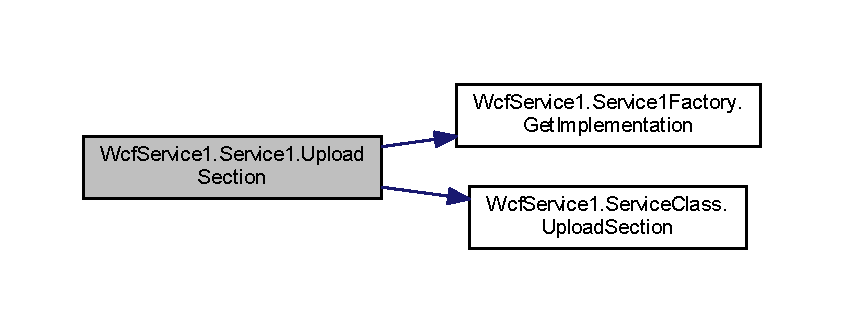
\includegraphics[width=350pt]{class_wcf_service1_1_1_service1_a4ba31cd1a202c84fac4d03461d8f4361_cgraph}
\end{center}
\end{figure}




\subsection{Member Data Documentation}
\index{Wcf\+Service1\+::\+Service1@{Wcf\+Service1\+::\+Service1}!factory@{factory}}
\index{factory@{factory}!Wcf\+Service1\+::\+Service1@{Wcf\+Service1\+::\+Service1}}
\subsubsection[{\texorpdfstring{factory}{factory}}]{\setlength{\rightskip}{0pt plus 5cm}{\bf Service1\+Factory} Wcf\+Service1.\+Service1.\+factory = new {\bf Service1\+Factory}(true)\hspace{0.3cm}{\ttfamily [private]}}\hypertarget{class_wcf_service1_1_1_service1_a7ff9458393176c80aa7d4365896de3b0}{}\label{class_wcf_service1_1_1_service1_a7ff9458393176c80aa7d4365896de3b0}


Factory returning the Mock Document(param true) or the real Document(param false) 



The documentation for this class was generated from the following file\+:\begin{DoxyCompactItemize}
\item 
C\+:/\+Users/user/source/repos/\+Hoermirzu/\+Listen\+To\+Me-\/master-\/89f0b49594deaade7bfad24dad062ff16eca36da/\+Wcf\+Service1/\hyperlink{_service1_8svc_8cs}{Service1.\+svc.\+cs}\end{DoxyCompactItemize}

\hypertarget{class_wcf_service1_1_1_service1_factory}{}\section{Wcf\+Service1.\+Service1\+Factory Class Reference}
\label{class_wcf_service1_1_1_service1_factory}\index{Wcf\+Service1.\+Service1\+Factory@{Wcf\+Service1.\+Service1\+Factory}}


Inheritance diagram for Wcf\+Service1.\+Service1\+Factory\+:\nopagebreak
\begin{figure}[H]
\begin{center}
\leavevmode
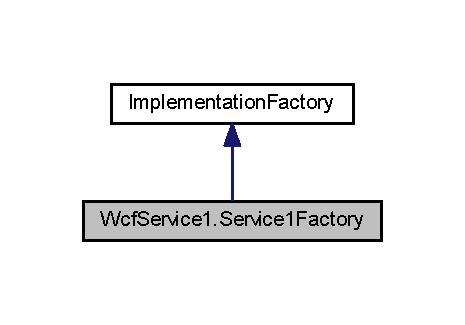
\includegraphics[width=223pt]{class_wcf_service1_1_1_service1_factory__inherit__graph}
\end{center}
\end{figure}


Collaboration diagram for Wcf\+Service1.\+Service1\+Factory\+:\nopagebreak
\begin{figure}[H]
\begin{center}
\leavevmode
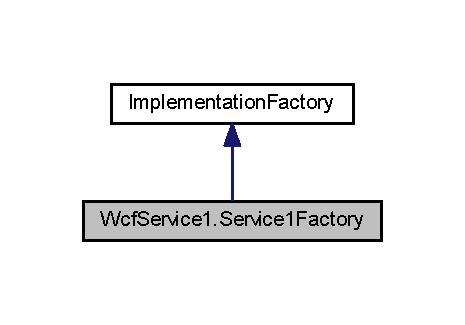
\includegraphics[width=223pt]{class_wcf_service1_1_1_service1_factory__coll__graph}
\end{center}
\end{figure}
\subsection*{Public Member Functions}
\begin{DoxyCompactItemize}
\item 
\hyperlink{class_wcf_service1_1_1_service1_factory_a7e56959270e8bda3cd348e86cd8e370d}{Service1\+Factory} ()
\item 
\hyperlink{class_wcf_service1_1_1_service1_factory_a3d585ca9f17bb7a01a96f82bcbf80bd4}{Service1\+Factory} (bool v)
\item 
override \hyperlink{class_wcf_service1_1_1_service_class}{Service\+Class} \hyperlink{class_wcf_service1_1_1_service1_factory_ae1204f90d6f8c4fcd4ad6b95cb6815b7}{Get\+Implementation} ()
\item 
Boolean \hyperlink{class_wcf_service1_1_1_service1_factory_ab93c8e9c9e2a60cfbeb00f3c67e4e364}{Get\+Mode} ()
\end{DoxyCompactItemize}
\subsection*{Private Attributes}
\begin{DoxyCompactItemize}
\item 
Boolean \hyperlink{class_wcf_service1_1_1_service1_factory_acc8fbf60ae4102452ad90ca06b8ffc45}{is\+Mock}
\end{DoxyCompactItemize}


\subsection{Constructor \& Destructor Documentation}
\index{Wcf\+Service1\+::\+Service1\+Factory@{Wcf\+Service1\+::\+Service1\+Factory}!Service1\+Factory@{Service1\+Factory}}
\index{Service1\+Factory@{Service1\+Factory}!Wcf\+Service1\+::\+Service1\+Factory@{Wcf\+Service1\+::\+Service1\+Factory}}
\subsubsection[{\texorpdfstring{Service1\+Factory()}{Service1Factory()}}]{\setlength{\rightskip}{0pt plus 5cm}Wcf\+Service1.\+Service1\+Factory.\+Service1\+Factory (
\begin{DoxyParamCaption}
{}
\end{DoxyParamCaption}
)}\hypertarget{class_wcf_service1_1_1_service1_factory_a7e56959270e8bda3cd348e86cd8e370d}{}\label{class_wcf_service1_1_1_service1_factory_a7e56959270e8bda3cd348e86cd8e370d}
\index{Wcf\+Service1\+::\+Service1\+Factory@{Wcf\+Service1\+::\+Service1\+Factory}!Service1\+Factory@{Service1\+Factory}}
\index{Service1\+Factory@{Service1\+Factory}!Wcf\+Service1\+::\+Service1\+Factory@{Wcf\+Service1\+::\+Service1\+Factory}}
\subsubsection[{\texorpdfstring{Service1\+Factory(bool v)}{Service1Factory(bool v)}}]{\setlength{\rightskip}{0pt plus 5cm}Wcf\+Service1.\+Service1\+Factory.\+Service1\+Factory (
\begin{DoxyParamCaption}
\item[{bool}]{v}
\end{DoxyParamCaption}
)}\hypertarget{class_wcf_service1_1_1_service1_factory_a3d585ca9f17bb7a01a96f82bcbf80bd4}{}\label{class_wcf_service1_1_1_service1_factory_a3d585ca9f17bb7a01a96f82bcbf80bd4}


\subsection{Member Function Documentation}
\index{Wcf\+Service1\+::\+Service1\+Factory@{Wcf\+Service1\+::\+Service1\+Factory}!Get\+Implementation@{Get\+Implementation}}
\index{Get\+Implementation@{Get\+Implementation}!Wcf\+Service1\+::\+Service1\+Factory@{Wcf\+Service1\+::\+Service1\+Factory}}
\subsubsection[{\texorpdfstring{Get\+Implementation()}{GetImplementation()}}]{\setlength{\rightskip}{0pt plus 5cm}override {\bf Service\+Class} Wcf\+Service1.\+Service1\+Factory.\+Get\+Implementation (
\begin{DoxyParamCaption}
{}
\end{DoxyParamCaption}
)\hspace{0.3cm}{\ttfamily [virtual]}}\hypertarget{class_wcf_service1_1_1_service1_factory_ae1204f90d6f8c4fcd4ad6b95cb6815b7}{}\label{class_wcf_service1_1_1_service1_factory_ae1204f90d6f8c4fcd4ad6b95cb6815b7}


Implements \hyperlink{class_wcf_service1_1_1_implementation_factory_ae88b463f0c749ded38d5cbcf2c1dd7cb}{Wcf\+Service1.\+Implementation\+Factory}.



Here is the caller graph for this function\+:\nopagebreak
\begin{figure}[H]
\begin{center}
\leavevmode
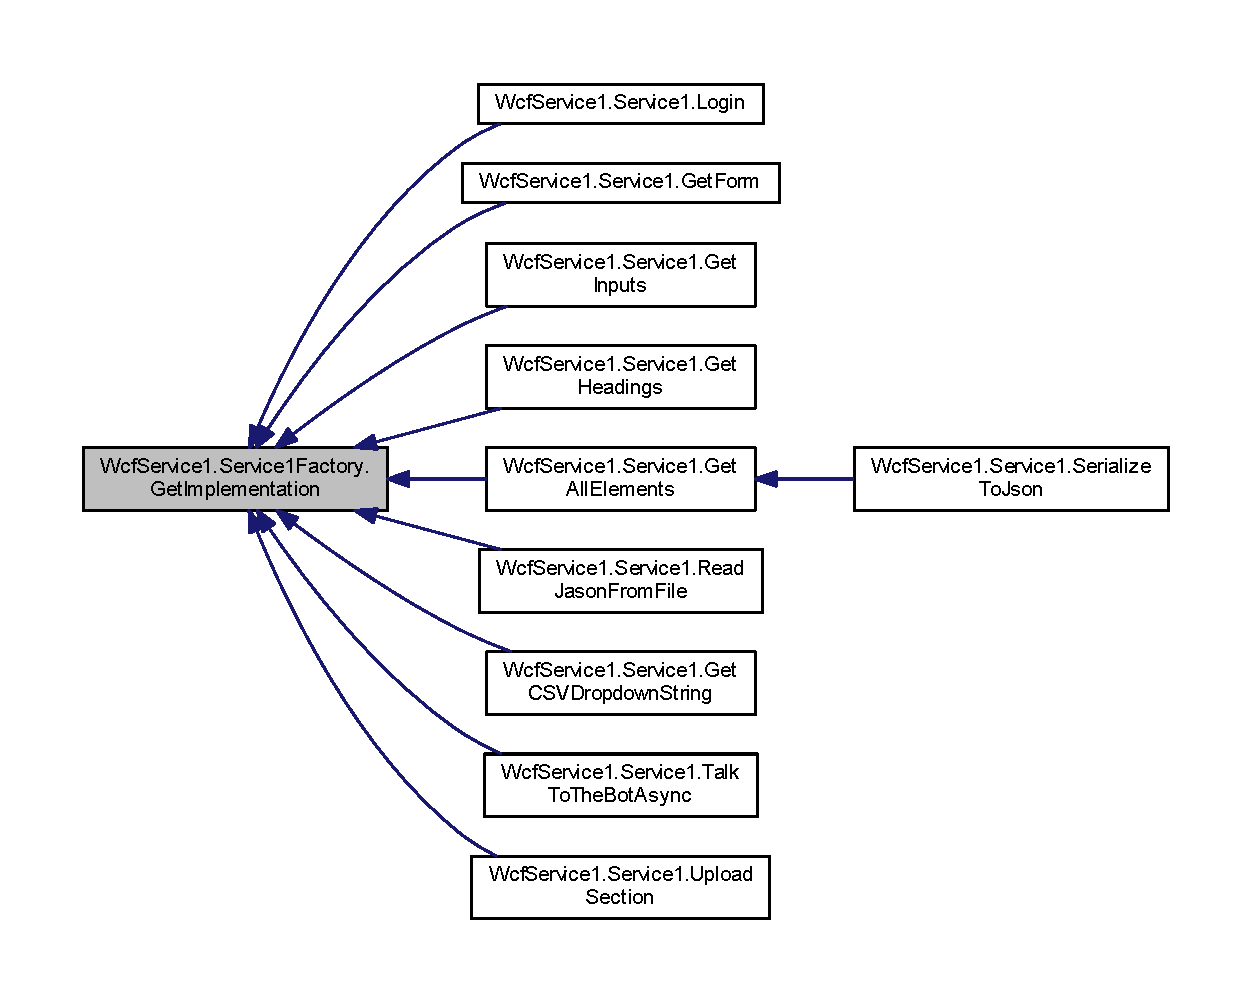
\includegraphics[width=350pt]{class_wcf_service1_1_1_service1_factory_ae1204f90d6f8c4fcd4ad6b95cb6815b7_icgraph}
\end{center}
\end{figure}


\index{Wcf\+Service1\+::\+Service1\+Factory@{Wcf\+Service1\+::\+Service1\+Factory}!Get\+Mode@{Get\+Mode}}
\index{Get\+Mode@{Get\+Mode}!Wcf\+Service1\+::\+Service1\+Factory@{Wcf\+Service1\+::\+Service1\+Factory}}
\subsubsection[{\texorpdfstring{Get\+Mode()}{GetMode()}}]{\setlength{\rightskip}{0pt plus 5cm}Boolean Wcf\+Service1.\+Service1\+Factory.\+Get\+Mode (
\begin{DoxyParamCaption}
{}
\end{DoxyParamCaption}
)}\hypertarget{class_wcf_service1_1_1_service1_factory_ab93c8e9c9e2a60cfbeb00f3c67e4e364}{}\label{class_wcf_service1_1_1_service1_factory_ab93c8e9c9e2a60cfbeb00f3c67e4e364}


\subsection{Member Data Documentation}
\index{Wcf\+Service1\+::\+Service1\+Factory@{Wcf\+Service1\+::\+Service1\+Factory}!is\+Mock@{is\+Mock}}
\index{is\+Mock@{is\+Mock}!Wcf\+Service1\+::\+Service1\+Factory@{Wcf\+Service1\+::\+Service1\+Factory}}
\subsubsection[{\texorpdfstring{is\+Mock}{isMock}}]{\setlength{\rightskip}{0pt plus 5cm}Boolean Wcf\+Service1.\+Service1\+Factory.\+is\+Mock\hspace{0.3cm}{\ttfamily [private]}}\hypertarget{class_wcf_service1_1_1_service1_factory_acc8fbf60ae4102452ad90ca06b8ffc45}{}\label{class_wcf_service1_1_1_service1_factory_acc8fbf60ae4102452ad90ca06b8ffc45}


The documentation for this class was generated from the following file\+:\begin{DoxyCompactItemize}
\item 
C\+:/\+Users/user/source/repos/\+Hoermirzu/\+Listen\+To\+Me-\/master-\/89f0b49594deaade7bfad24dad062ff16eca36da/\+Wcf\+Service1/\hyperlink{_implementation_factory_8cs}{Implementation\+Factory.\+cs}\end{DoxyCompactItemize}

\hypertarget{class_wcf_service1_1_1_service_class}{}\section{Wcf\+Service1.\+Service\+Class Class Reference}
\label{class_wcf_service1_1_1_service_class}\index{Wcf\+Service1.\+Service\+Class@{Wcf\+Service1.\+Service\+Class}}


contains operations of the service1client for parsing the html-\/webform All operations containing a \char`\"{}1\char`\"{} are Dummy-\/\+Operations that only run on files simulating the webform  




Inheritance diagram for Wcf\+Service1.\+Service\+Class\+:\nopagebreak
\begin{figure}[H]
\begin{center}
\leavevmode
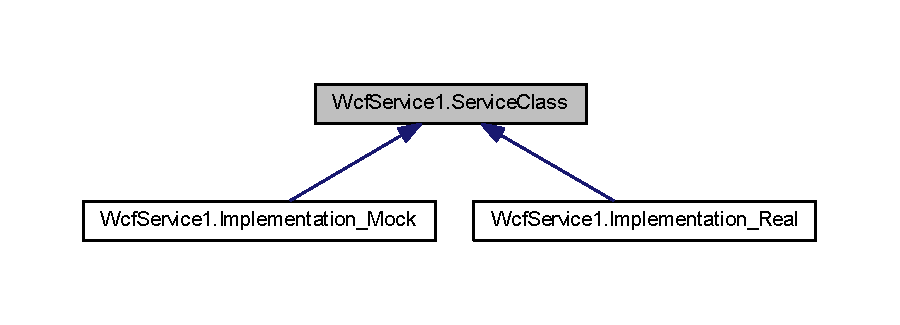
\includegraphics[width=350pt]{class_wcf_service1_1_1_service_class__inherit__graph}
\end{center}
\end{figure}


Collaboration diagram for Wcf\+Service1.\+Service\+Class\+:\nopagebreak
\begin{figure}[H]
\begin{center}
\leavevmode
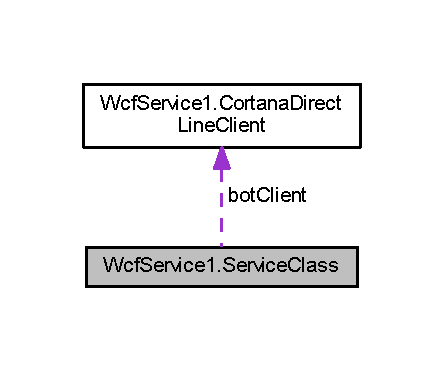
\includegraphics[width=213pt]{class_wcf_service1_1_1_service_class__coll__graph}
\end{center}
\end{figure}
\subsection*{Public Member Functions}
\begin{DoxyCompactItemize}
\item 
abstract bool \hyperlink{class_wcf_service1_1_1_service_class_add477e49eab8927cc943dfb751dc976a}{Upload\+Section} (Section section)
\item 
abstract string \hyperlink{class_wcf_service1_1_1_service_class_a023c63c6a95132c7f2b9754c1bb41c80}{Login} (string user\+Name, string password)
\item 
abstract string \hyperlink{class_wcf_service1_1_1_service_class_a791350c6bf7ba90f63f95e1b935dde3b}{Get\+Form} (string username, string password)
\item 
abstract List$<$ Section $>$ \hyperlink{class_wcf_service1_1_1_service_class_ac0640daeb28fada4b6f80a2b66b0ec3e}{Get\+All\+Elements} (string username, string password)
\item 
async Task$<$ string $>$ \hyperlink{class_wcf_service1_1_1_service_class_a9c82b9884f5da75aad18624ff0f74115}{Talk\+To\+The\+Bot\+Async} (string message)
\item 
List$<$ string $>$ \hyperlink{class_wcf_service1_1_1_service_class_a4ad3ab638087f1c0deaeafcd5de0592c}{Get\+Headings} (string username, string password, string domain)
\item 
List$<$ string $>$ \hyperlink{class_wcf_service1_1_1_service_class_af7c843fb65336f76c29c1ce7633d3f18}{Get\+Inputs} (string username, string password, string domain)
\begin{DoxyCompactList}\small\item\em returns a list of all labels on the web form. Those can then be translated into text\+Boxes by the App \end{DoxyCompactList}\item 
string \hyperlink{class_wcf_service1_1_1_service_class_a3911ec2648b29d1ed247ee852920ca62}{Read\+File} (string filename)
\item 
string \hyperlink{class_wcf_service1_1_1_service_class_abc1e643d4f507b20ddb1c477e0ec3307}{Get\+C\+S\+V\+Dropdown\+String} (string list\+\_\+id)
\end{DoxyCompactItemize}
\subsection*{Private Member Functions}
\begin{DoxyCompactItemize}
\item 
string \hyperlink{class_wcf_service1_1_1_service_class_ab88a7ee56c72aac3229b737273fbca20}{Read\+Lines\+Containing\+String} (string list\+\_\+id, File\+Info file)
\begin{DoxyCompactList}\small\item\em retrieves the dropdown menu lines for a specific drobdown menu \end{DoxyCompactList}\end{DoxyCompactItemize}
\subsection*{Private Attributes}
\begin{DoxyCompactItemize}
\item 
\hyperlink{class_wcf_service1_1_1_cortana_direct_line_client}{Cortana\+Direct\+Line\+Client} \hyperlink{class_wcf_service1_1_1_service_class_a9bd8bdea6c82d92334badcb56a75d0a8}{bot\+Client} = new \hyperlink{class_wcf_service1_1_1_cortana_direct_line_client}{Cortana\+Direct\+Line\+Client}()
\begin{DoxyCompactList}\small\item\em connects to the bot using Direct\+Line \end{DoxyCompactList}\end{DoxyCompactItemize}


\subsection{Detailed Description}
contains operations of the service1client for parsing the html-\/webform All operations containing a \char`\"{}1\char`\"{} are Dummy-\/\+Operations that only run on files simulating the webform 



\subsection{Member Function Documentation}
\index{Wcf\+Service1\+::\+Service\+Class@{Wcf\+Service1\+::\+Service\+Class}!Get\+All\+Elements@{Get\+All\+Elements}}
\index{Get\+All\+Elements@{Get\+All\+Elements}!Wcf\+Service1\+::\+Service\+Class@{Wcf\+Service1\+::\+Service\+Class}}
\subsubsection[{\texorpdfstring{Get\+All\+Elements(string username, string password)}{GetAllElements(string username, string password)}}]{\setlength{\rightskip}{0pt plus 5cm}abstract List$<$Section$>$ Wcf\+Service1.\+Service\+Class.\+Get\+All\+Elements (
\begin{DoxyParamCaption}
\item[{string}]{username, }
\item[{string}]{password}
\end{DoxyParamCaption}
)\hspace{0.3cm}{\ttfamily [pure virtual]}}\hypertarget{class_wcf_service1_1_1_service_class_ac0640daeb28fada4b6f80a2b66b0ec3e}{}\label{class_wcf_service1_1_1_service_class_ac0640daeb28fada4b6f80a2b66b0ec3e}


Implemented in \hyperlink{class_wcf_service1_1_1_implementation___mock_a3677cf44f7acac9549f1e58ce9191e4e}{Wcf\+Service1.\+Implementation\+\_\+\+Mock}, and \hyperlink{class_wcf_service1_1_1_implementation___real_a6cedd1da2b421038727ed52afaf7197e}{Wcf\+Service1.\+Implementation\+\_\+\+Real}.



Here is the caller graph for this function\+:\nopagebreak
\begin{figure}[H]
\begin{center}
\leavevmode
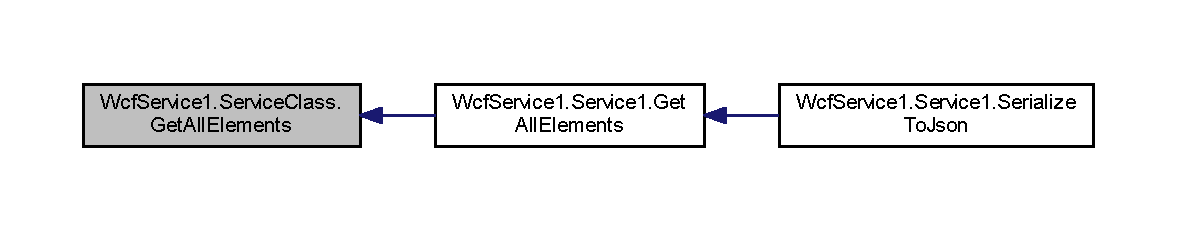
\includegraphics[width=350pt]{class_wcf_service1_1_1_service_class_ac0640daeb28fada4b6f80a2b66b0ec3e_icgraph}
\end{center}
\end{figure}


\index{Wcf\+Service1\+::\+Service\+Class@{Wcf\+Service1\+::\+Service\+Class}!Get\+C\+S\+V\+Dropdown\+String@{Get\+C\+S\+V\+Dropdown\+String}}
\index{Get\+C\+S\+V\+Dropdown\+String@{Get\+C\+S\+V\+Dropdown\+String}!Wcf\+Service1\+::\+Service\+Class@{Wcf\+Service1\+::\+Service\+Class}}
\subsubsection[{\texorpdfstring{Get\+C\+S\+V\+Dropdown\+String(string list\+\_\+id)}{GetCSVDropdownString(string list_id)}}]{\setlength{\rightskip}{0pt plus 5cm}string Wcf\+Service1.\+Service\+Class.\+Get\+C\+S\+V\+Dropdown\+String (
\begin{DoxyParamCaption}
\item[{string}]{list\+\_\+id}
\end{DoxyParamCaption}
)}\hypertarget{class_wcf_service1_1_1_service_class_abc1e643d4f507b20ddb1c477e0ec3307}{}\label{class_wcf_service1_1_1_service_class_abc1e643d4f507b20ddb1c477e0ec3307}


Here is the call graph for this function\+:\nopagebreak
\begin{figure}[H]
\begin{center}
\leavevmode
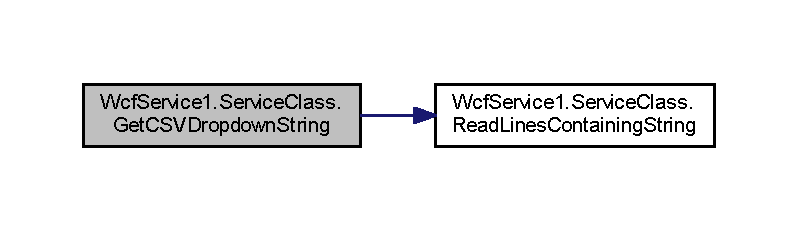
\includegraphics[width=350pt]{class_wcf_service1_1_1_service_class_abc1e643d4f507b20ddb1c477e0ec3307_cgraph}
\end{center}
\end{figure}




Here is the caller graph for this function\+:\nopagebreak
\begin{figure}[H]
\begin{center}
\leavevmode
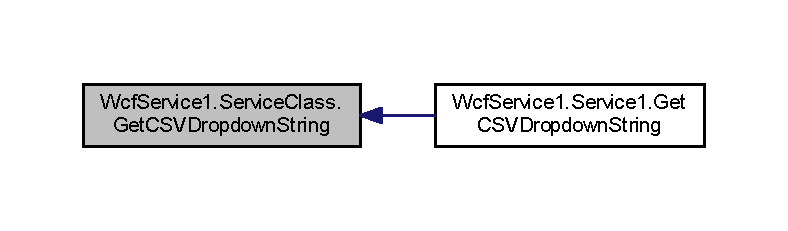
\includegraphics[width=350pt]{class_wcf_service1_1_1_service_class_abc1e643d4f507b20ddb1c477e0ec3307_icgraph}
\end{center}
\end{figure}


\index{Wcf\+Service1\+::\+Service\+Class@{Wcf\+Service1\+::\+Service\+Class}!Get\+Form@{Get\+Form}}
\index{Get\+Form@{Get\+Form}!Wcf\+Service1\+::\+Service\+Class@{Wcf\+Service1\+::\+Service\+Class}}
\subsubsection[{\texorpdfstring{Get\+Form(string username, string password)}{GetForm(string username, string password)}}]{\setlength{\rightskip}{0pt plus 5cm}abstract string Wcf\+Service1.\+Service\+Class.\+Get\+Form (
\begin{DoxyParamCaption}
\item[{string}]{username, }
\item[{string}]{password}
\end{DoxyParamCaption}
)\hspace{0.3cm}{\ttfamily [pure virtual]}}\hypertarget{class_wcf_service1_1_1_service_class_a791350c6bf7ba90f63f95e1b935dde3b}{}\label{class_wcf_service1_1_1_service_class_a791350c6bf7ba90f63f95e1b935dde3b}


Implemented in \hyperlink{class_wcf_service1_1_1_implementation___real_a82b0d0cc9a634454bfa583f55eb13dad}{Wcf\+Service1.\+Implementation\+\_\+\+Real}, and \hyperlink{class_wcf_service1_1_1_implementation___mock_a770d195f0883f20e2356381152a6ea00}{Wcf\+Service1.\+Implementation\+\_\+\+Mock}.



Here is the caller graph for this function\+:\nopagebreak
\begin{figure}[H]
\begin{center}
\leavevmode
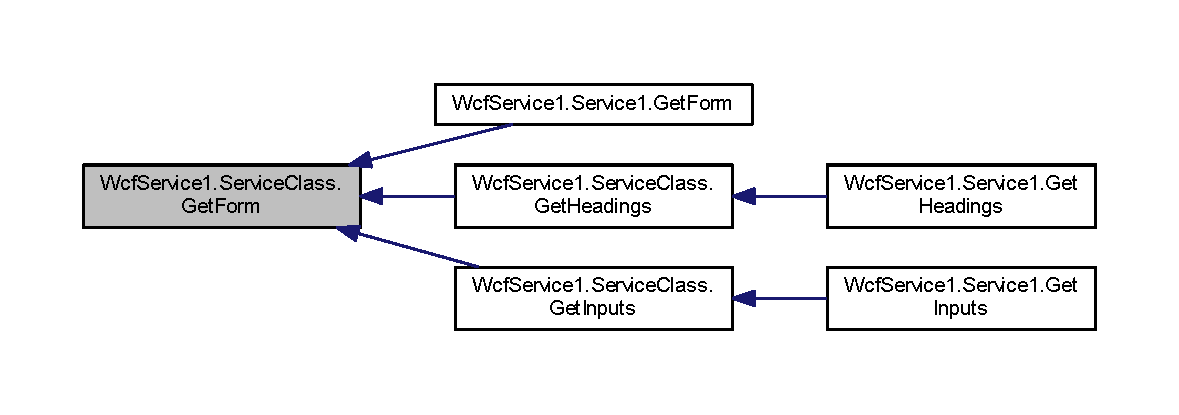
\includegraphics[width=350pt]{class_wcf_service1_1_1_service_class_a791350c6bf7ba90f63f95e1b935dde3b_icgraph}
\end{center}
\end{figure}


\index{Wcf\+Service1\+::\+Service\+Class@{Wcf\+Service1\+::\+Service\+Class}!Get\+Headings@{Get\+Headings}}
\index{Get\+Headings@{Get\+Headings}!Wcf\+Service1\+::\+Service\+Class@{Wcf\+Service1\+::\+Service\+Class}}
\subsubsection[{\texorpdfstring{Get\+Headings(string username, string password, string domain)}{GetHeadings(string username, string password, string domain)}}]{\setlength{\rightskip}{0pt plus 5cm}List$<$string$>$ Wcf\+Service1.\+Service\+Class.\+Get\+Headings (
\begin{DoxyParamCaption}
\item[{string}]{username, }
\item[{string}]{password, }
\item[{string}]{domain}
\end{DoxyParamCaption}
)}\hypertarget{class_wcf_service1_1_1_service_class_a4ad3ab638087f1c0deaeafcd5de0592c}{}\label{class_wcf_service1_1_1_service_class_a4ad3ab638087f1c0deaeafcd5de0592c}


Here is the call graph for this function\+:\nopagebreak
\begin{figure}[H]
\begin{center}
\leavevmode
\includegraphics[width=350pt]{class_wcf_service1_1_1_service_class_a4ad3ab638087f1c0deaeafcd5de0592c_cgraph}
\end{center}
\end{figure}




Here is the caller graph for this function\+:\nopagebreak
\begin{figure}[H]
\begin{center}
\leavevmode
\includegraphics[width=350pt]{class_wcf_service1_1_1_service_class_a4ad3ab638087f1c0deaeafcd5de0592c_icgraph}
\end{center}
\end{figure}


\index{Wcf\+Service1\+::\+Service\+Class@{Wcf\+Service1\+::\+Service\+Class}!Get\+Inputs@{Get\+Inputs}}
\index{Get\+Inputs@{Get\+Inputs}!Wcf\+Service1\+::\+Service\+Class@{Wcf\+Service1\+::\+Service\+Class}}
\subsubsection[{\texorpdfstring{Get\+Inputs(string username, string password, string domain)}{GetInputs(string username, string password, string domain)}}]{\setlength{\rightskip}{0pt plus 5cm}List$<$string$>$ Wcf\+Service1.\+Service\+Class.\+Get\+Inputs (
\begin{DoxyParamCaption}
\item[{string}]{username, }
\item[{string}]{password, }
\item[{string}]{domain}
\end{DoxyParamCaption}
)}\hypertarget{class_wcf_service1_1_1_service_class_af7c843fb65336f76c29c1ce7633d3f18}{}\label{class_wcf_service1_1_1_service_class_af7c843fb65336f76c29c1ce7633d3f18}


returns a list of all labels on the web form. Those can then be translated into text\+Boxes by the App 


\begin{DoxyParams}{Parameters}
{\em username} & \\
\hline
{\em password} & \\
\hline
{\em domain} & \\
\hline
\end{DoxyParams}
\begin{DoxyReturn}{Returns}

\end{DoxyReturn}


Here is the call graph for this function\+:\nopagebreak
\begin{figure}[H]
\begin{center}
\leavevmode
\includegraphics[width=350pt]{class_wcf_service1_1_1_service_class_af7c843fb65336f76c29c1ce7633d3f18_cgraph}
\end{center}
\end{figure}




Here is the caller graph for this function\+:\nopagebreak
\begin{figure}[H]
\begin{center}
\leavevmode
\includegraphics[width=350pt]{class_wcf_service1_1_1_service_class_af7c843fb65336f76c29c1ce7633d3f18_icgraph}
\end{center}
\end{figure}


\index{Wcf\+Service1\+::\+Service\+Class@{Wcf\+Service1\+::\+Service\+Class}!Login@{Login}}
\index{Login@{Login}!Wcf\+Service1\+::\+Service\+Class@{Wcf\+Service1\+::\+Service\+Class}}
\subsubsection[{\texorpdfstring{Login(string user\+Name, string password)}{Login(string userName, string password)}}]{\setlength{\rightskip}{0pt plus 5cm}abstract string Wcf\+Service1.\+Service\+Class.\+Login (
\begin{DoxyParamCaption}
\item[{string}]{user\+Name, }
\item[{string}]{password}
\end{DoxyParamCaption}
)\hspace{0.3cm}{\ttfamily [pure virtual]}}\hypertarget{class_wcf_service1_1_1_service_class_a023c63c6a95132c7f2b9754c1bb41c80}{}\label{class_wcf_service1_1_1_service_class_a023c63c6a95132c7f2b9754c1bb41c80}


Implemented in \hyperlink{class_wcf_service1_1_1_implementation___real_aec1081c3a83135e9f11ea182ca3e9321}{Wcf\+Service1.\+Implementation\+\_\+\+Real}, and \hyperlink{class_wcf_service1_1_1_implementation___mock_ad4676c509d48e01e7ed6e2962fc01b29}{Wcf\+Service1.\+Implementation\+\_\+\+Mock}.



Here is the caller graph for this function\+:\nopagebreak
\begin{figure}[H]
\begin{center}
\leavevmode
\includegraphics[width=350pt]{class_wcf_service1_1_1_service_class_a023c63c6a95132c7f2b9754c1bb41c80_icgraph}
\end{center}
\end{figure}


\index{Wcf\+Service1\+::\+Service\+Class@{Wcf\+Service1\+::\+Service\+Class}!Read\+File@{Read\+File}}
\index{Read\+File@{Read\+File}!Wcf\+Service1\+::\+Service\+Class@{Wcf\+Service1\+::\+Service\+Class}}
\subsubsection[{\texorpdfstring{Read\+File(string filename)}{ReadFile(string filename)}}]{\setlength{\rightskip}{0pt plus 5cm}string Wcf\+Service1.\+Service\+Class.\+Read\+File (
\begin{DoxyParamCaption}
\item[{string}]{filename}
\end{DoxyParamCaption}
)}\hypertarget{class_wcf_service1_1_1_service_class_a3911ec2648b29d1ed247ee852920ca62}{}\label{class_wcf_service1_1_1_service_class_a3911ec2648b29d1ed247ee852920ca62}


Here is the caller graph for this function\+:\nopagebreak
\begin{figure}[H]
\begin{center}
\leavevmode
\includegraphics[width=350pt]{class_wcf_service1_1_1_service_class_a3911ec2648b29d1ed247ee852920ca62_icgraph}
\end{center}
\end{figure}


\index{Wcf\+Service1\+::\+Service\+Class@{Wcf\+Service1\+::\+Service\+Class}!Read\+Lines\+Containing\+String@{Read\+Lines\+Containing\+String}}
\index{Read\+Lines\+Containing\+String@{Read\+Lines\+Containing\+String}!Wcf\+Service1\+::\+Service\+Class@{Wcf\+Service1\+::\+Service\+Class}}
\subsubsection[{\texorpdfstring{Read\+Lines\+Containing\+String(string list\+\_\+id, File\+Info file)}{ReadLinesContainingString(string list_id, FileInfo file)}}]{\setlength{\rightskip}{0pt plus 5cm}string Wcf\+Service1.\+Service\+Class.\+Read\+Lines\+Containing\+String (
\begin{DoxyParamCaption}
\item[{string}]{list\+\_\+id, }
\item[{File\+Info}]{file}
\end{DoxyParamCaption}
)\hspace{0.3cm}{\ttfamily [private]}}\hypertarget{class_wcf_service1_1_1_service_class_ab88a7ee56c72aac3229b737273fbca20}{}\label{class_wcf_service1_1_1_service_class_ab88a7ee56c72aac3229b737273fbca20}


retrieves the dropdown menu lines for a specific drobdown menu 


\begin{DoxyParams}{Parameters}
{\em list\+\_\+id} & \\
\hline
{\em file} & \\
\hline
\end{DoxyParams}
\begin{DoxyReturn}{Returns}

\end{DoxyReturn}


Here is the caller graph for this function\+:\nopagebreak
\begin{figure}[H]
\begin{center}
\leavevmode
\includegraphics[width=350pt]{class_wcf_service1_1_1_service_class_ab88a7ee56c72aac3229b737273fbca20_icgraph}
\end{center}
\end{figure}


\index{Wcf\+Service1\+::\+Service\+Class@{Wcf\+Service1\+::\+Service\+Class}!Talk\+To\+The\+Bot\+Async@{Talk\+To\+The\+Bot\+Async}}
\index{Talk\+To\+The\+Bot\+Async@{Talk\+To\+The\+Bot\+Async}!Wcf\+Service1\+::\+Service\+Class@{Wcf\+Service1\+::\+Service\+Class}}
\subsubsection[{\texorpdfstring{Talk\+To\+The\+Bot\+Async(string message)}{TalkToTheBotAsync(string message)}}]{\setlength{\rightskip}{0pt plus 5cm}async Task$<$string$>$ Wcf\+Service1.\+Service\+Class.\+Talk\+To\+The\+Bot\+Async (
\begin{DoxyParamCaption}
\item[{string}]{message}
\end{DoxyParamCaption}
)}\hypertarget{class_wcf_service1_1_1_service_class_a9c82b9884f5da75aad18624ff0f74115}{}\label{class_wcf_service1_1_1_service_class_a9c82b9884f5da75aad18624ff0f74115}


Here is the call graph for this function\+:\nopagebreak
\begin{figure}[H]
\begin{center}
\leavevmode
\includegraphics[width=350pt]{class_wcf_service1_1_1_service_class_a9c82b9884f5da75aad18624ff0f74115_cgraph}
\end{center}
\end{figure}




Here is the caller graph for this function\+:\nopagebreak
\begin{figure}[H]
\begin{center}
\leavevmode
\includegraphics[width=350pt]{class_wcf_service1_1_1_service_class_a9c82b9884f5da75aad18624ff0f74115_icgraph}
\end{center}
\end{figure}


\index{Wcf\+Service1\+::\+Service\+Class@{Wcf\+Service1\+::\+Service\+Class}!Upload\+Section@{Upload\+Section}}
\index{Upload\+Section@{Upload\+Section}!Wcf\+Service1\+::\+Service\+Class@{Wcf\+Service1\+::\+Service\+Class}}
\subsubsection[{\texorpdfstring{Upload\+Section(\+Section section)}{UploadSection(Section section)}}]{\setlength{\rightskip}{0pt plus 5cm}abstract bool Wcf\+Service1.\+Service\+Class.\+Upload\+Section (
\begin{DoxyParamCaption}
\item[{Section}]{section}
\end{DoxyParamCaption}
)\hspace{0.3cm}{\ttfamily [pure virtual]}}\hypertarget{class_wcf_service1_1_1_service_class_add477e49eab8927cc943dfb751dc976a}{}\label{class_wcf_service1_1_1_service_class_add477e49eab8927cc943dfb751dc976a}


Implemented in \hyperlink{class_wcf_service1_1_1_implementation___real_ac95892552f6beb92e0557abde468a5a1}{Wcf\+Service1.\+Implementation\+\_\+\+Real}, and \hyperlink{class_wcf_service1_1_1_implementation___mock_aacbbae5d5cd842b1c62cfab84168b287}{Wcf\+Service1.\+Implementation\+\_\+\+Mock}.



Here is the caller graph for this function\+:\nopagebreak
\begin{figure}[H]
\begin{center}
\leavevmode
\includegraphics[width=350pt]{class_wcf_service1_1_1_service_class_add477e49eab8927cc943dfb751dc976a_icgraph}
\end{center}
\end{figure}




\subsection{Member Data Documentation}
\index{Wcf\+Service1\+::\+Service\+Class@{Wcf\+Service1\+::\+Service\+Class}!bot\+Client@{bot\+Client}}
\index{bot\+Client@{bot\+Client}!Wcf\+Service1\+::\+Service\+Class@{Wcf\+Service1\+::\+Service\+Class}}
\subsubsection[{\texorpdfstring{bot\+Client}{botClient}}]{\setlength{\rightskip}{0pt plus 5cm}{\bf Cortana\+Direct\+Line\+Client} Wcf\+Service1.\+Service\+Class.\+bot\+Client = new {\bf Cortana\+Direct\+Line\+Client}()\hspace{0.3cm}{\ttfamily [private]}}\hypertarget{class_wcf_service1_1_1_service_class_a9bd8bdea6c82d92334badcb56a75d0a8}{}\label{class_wcf_service1_1_1_service_class_a9bd8bdea6c82d92334badcb56a75d0a8}


connects to the bot using Direct\+Line 



The documentation for this class was generated from the following file\+:\begin{DoxyCompactItemize}
\item 
C\+:/\+Users/user/source/repos/\+Hoermirzu/\+Listen\+To\+Me-\/master-\/89f0b49594deaade7bfad24dad062ff16eca36da/\+Wcf\+Service1/\hyperlink{_service_class_8cs}{Service\+Class.\+cs}\end{DoxyCompactItemize}

\hypertarget{class_wcf_service1_1_1_website_crawler}{}\section{Wcf\+Service1.\+Website\+Crawler Class Reference}
\label{class_wcf_service1_1_1_website_crawler}\index{Wcf\+Service1.\+Website\+Crawler@{Wcf\+Service1.\+Website\+Crawler}}


this class is opening a connection to the web form. I provides methods for retreiving the H\+T\+M\+L-\/\+Code behind a spechific form.  


\subsection*{Public Member Functions}
\begin{DoxyCompactItemize}
\item 
string \hyperlink{class_wcf_service1_1_1_website_crawler_afb8f0be0431c8622a8071d8ee088601e}{get\+Web\+Content\+Persist} (string url, string finished\+Condition=null)
\item 
string \hyperlink{class_wcf_service1_1_1_website_crawler_a53d529051737c346206af942b7c06763}{get\+Web\+Content} (string url, string finished\+Condition=null, List$<$ Cookie $>$ cookies=null)
\begin{DoxyCompactList}\small\item\em same thing with cookies, but it doesn\textquotesingle{}t work todo debug \end{DoxyCompactList}\end{DoxyCompactItemize}
\subsection*{Static Private Attributes}
\begin{DoxyCompactItemize}
\item 
static Phantom\+J\+S\+Driver \hyperlink{class_wcf_service1_1_1_website_crawler_a19b2a7a21595cee4f8a9317add3bc0b0}{persisting\+Phantom\+Driver} = new Phantom\+J\+S\+Driver()
\end{DoxyCompactItemize}


\subsection{Detailed Description}
this class is opening a connection to the web form. I provides methods for retreiving the H\+T\+M\+L-\/\+Code behind a spechific form. 



\subsection{Member Function Documentation}
\index{Wcf\+Service1\+::\+Website\+Crawler@{Wcf\+Service1\+::\+Website\+Crawler}!get\+Web\+Content@{get\+Web\+Content}}
\index{get\+Web\+Content@{get\+Web\+Content}!Wcf\+Service1\+::\+Website\+Crawler@{Wcf\+Service1\+::\+Website\+Crawler}}
\subsubsection[{\texorpdfstring{get\+Web\+Content(string url, string finished\+Condition=null, List$<$ Cookie $>$ cookies=null)}{getWebContent(string url, string finishedCondition=null, List< Cookie > cookies=null)}}]{\setlength{\rightskip}{0pt plus 5cm}string Wcf\+Service1.\+Website\+Crawler.\+get\+Web\+Content (
\begin{DoxyParamCaption}
\item[{string}]{url, }
\item[{string}]{finished\+Condition = {\ttfamily null}, }
\item[{List$<$ Cookie $>$}]{cookies = {\ttfamily null}}
\end{DoxyParamCaption}
)}\hypertarget{class_wcf_service1_1_1_website_crawler_a53d529051737c346206af942b7c06763}{}\label{class_wcf_service1_1_1_website_crawler_a53d529051737c346206af942b7c06763}


same thing with cookies, but it doesn\textquotesingle{}t work todo debug 


\begin{DoxyParams}{Parameters}
{\em url} & \\
\hline
{\em finished\+Condition} & \\
\hline
{\em cookies} & \\
\hline
\end{DoxyParams}
\begin{DoxyReturn}{Returns}

\end{DoxyReturn}
\index{Wcf\+Service1\+::\+Website\+Crawler@{Wcf\+Service1\+::\+Website\+Crawler}!get\+Web\+Content\+Persist@{get\+Web\+Content\+Persist}}
\index{get\+Web\+Content\+Persist@{get\+Web\+Content\+Persist}!Wcf\+Service1\+::\+Website\+Crawler@{Wcf\+Service1\+::\+Website\+Crawler}}
\subsubsection[{\texorpdfstring{get\+Web\+Content\+Persist(string url, string finished\+Condition=null)}{getWebContentPersist(string url, string finishedCondition=null)}}]{\setlength{\rightskip}{0pt plus 5cm}string Wcf\+Service1.\+Website\+Crawler.\+get\+Web\+Content\+Persist (
\begin{DoxyParamCaption}
\item[{string}]{url, }
\item[{string}]{finished\+Condition = {\ttfamily null}}
\end{DoxyParamCaption}
)}\hypertarget{class_wcf_service1_1_1_website_crawler_afb8f0be0431c8622a8071d8ee088601e}{}\label{class_wcf_service1_1_1_website_crawler_afb8f0be0431c8622a8071d8ee088601e}


Here is the caller graph for this function\+:\nopagebreak
\begin{figure}[H]
\begin{center}
\leavevmode
\includegraphics[width=350pt]{class_wcf_service1_1_1_website_crawler_afb8f0be0431c8622a8071d8ee088601e_icgraph}
\end{center}
\end{figure}




\subsection{Member Data Documentation}
\index{Wcf\+Service1\+::\+Website\+Crawler@{Wcf\+Service1\+::\+Website\+Crawler}!persisting\+Phantom\+Driver@{persisting\+Phantom\+Driver}}
\index{persisting\+Phantom\+Driver@{persisting\+Phantom\+Driver}!Wcf\+Service1\+::\+Website\+Crawler@{Wcf\+Service1\+::\+Website\+Crawler}}
\subsubsection[{\texorpdfstring{persisting\+Phantom\+Driver}{persistingPhantomDriver}}]{\setlength{\rightskip}{0pt plus 5cm}Phantom\+J\+S\+Driver Wcf\+Service1.\+Website\+Crawler.\+persisting\+Phantom\+Driver = new Phantom\+J\+S\+Driver()\hspace{0.3cm}{\ttfamily [static]}, {\ttfamily [private]}}\hypertarget{class_wcf_service1_1_1_website_crawler_a19b2a7a21595cee4f8a9317add3bc0b0}{}\label{class_wcf_service1_1_1_website_crawler_a19b2a7a21595cee4f8a9317add3bc0b0}


The documentation for this class was generated from the following file\+:\begin{DoxyCompactItemize}
\item 
C\+:/\+Users/user/source/repos/\+Hoermirzu/\+Listen\+To\+Me-\/master-\/89f0b49594deaade7bfad24dad062ff16eca36da/\+Wcf\+Service1/\hyperlink{_website_crawler_8cs}{Website\+Crawler.\+cs}\end{DoxyCompactItemize}

\chapter{File Documentation}
\hypertarget{_alexa_8cs}{}\section{C\+:/\+Users/user/source/repos/\+Hoermirzu/\+Listen\+To\+Me-\/master-\/89f0b49594deaade7bfad24dad062ff16eca36da/\+Wcf\+Service1/\+Alexa.cs File Reference}
\label{_alexa_8cs}\index{C\+:/\+Users/user/source/repos/\+Hoermirzu/\+Listen\+To\+Me-\/master-\/89f0b49594deaade7bfad24dad062ff16eca36da/\+Wcf\+Service1/\+Alexa.\+cs@{C\+:/\+Users/user/source/repos/\+Hoermirzu/\+Listen\+To\+Me-\/master-\/89f0b49594deaade7bfad24dad062ff16eca36da/\+Wcf\+Service1/\+Alexa.\+cs}}
\subsection*{Classes}
\begin{DoxyCompactItemize}
\item 
class \hyperlink{class_wcf_service1_1_1_alexa}{Wcf\+Service1.\+Alexa}
\begin{DoxyCompactList}\small\item\em provides code for connecting to an \hyperlink{class_wcf_service1_1_1_alexa}{Alexa} skill. Not tested. reference\+: \href{https://www.robinosborne.co.uk/2016/12/19/connecting-alexa-to-a-botframework-chatbot/}{\tt https\+://www.\+robinosborne.\+co.\+uk/2016/12/19/connecting-\/alexa-\/to-\/a-\/botframework-\/chatbot/} \end{DoxyCompactList}\end{DoxyCompactItemize}
\subsection*{Namespaces}
\begin{DoxyCompactItemize}
\item 
namespace \hyperlink{namespace_wcf_service1}{Wcf\+Service1}
\end{DoxyCompactItemize}

\hypertarget{_cortana_direct_line_client_8cs}{}\section{C\+:/\+Users/user/source/repos/\+Hoermirzu/\+Listen\+To\+Me-\/master-\/89f0b49594deaade7bfad24dad062ff16eca36da/\+Wcf\+Service1/\+Cortana\+Direct\+Line\+Client.cs File Reference}
\label{_cortana_direct_line_client_8cs}\index{C\+:/\+Users/user/source/repos/\+Hoermirzu/\+Listen\+To\+Me-\/master-\/89f0b49594deaade7bfad24dad062ff16eca36da/\+Wcf\+Service1/\+Cortana\+Direct\+Line\+Client.\+cs@{C\+:/\+Users/user/source/repos/\+Hoermirzu/\+Listen\+To\+Me-\/master-\/89f0b49594deaade7bfad24dad062ff16eca36da/\+Wcf\+Service1/\+Cortana\+Direct\+Line\+Client.\+cs}}
\subsection*{Classes}
\begin{DoxyCompactItemize}
\item 
class \hyperlink{class_wcf_service1_1_1_cortana_direct_line_client}{Wcf\+Service1.\+Cortana\+Direct\+Line\+Client}
\begin{DoxyCompactList}\small\item\em creates Direct\+Line connection to the bot \end{DoxyCompactList}\end{DoxyCompactItemize}
\subsection*{Namespaces}
\begin{DoxyCompactItemize}
\item 
namespace \hyperlink{namespace_wcf_service1}{Wcf\+Service1}
\end{DoxyCompactItemize}

\hypertarget{_implementation___mock_8cs}{}\section{C\+:/\+Users/user/source/repos/\+Hoermirzu/\+Listen\+To\+Me-\/master-\/89f0b49594deaade7bfad24dad062ff16eca36da/\+Wcf\+Service1/\+Implementation\+\_\+\+Mock.cs File Reference}
\label{_implementation___mock_8cs}\index{C\+:/\+Users/user/source/repos/\+Hoermirzu/\+Listen\+To\+Me-\/master-\/89f0b49594deaade7bfad24dad062ff16eca36da/\+Wcf\+Service1/\+Implementation\+\_\+\+Mock.\+cs@{C\+:/\+Users/user/source/repos/\+Hoermirzu/\+Listen\+To\+Me-\/master-\/89f0b49594deaade7bfad24dad062ff16eca36da/\+Wcf\+Service1/\+Implementation\+\_\+\+Mock.\+cs}}
\subsection*{Classes}
\begin{DoxyCompactItemize}
\item 
class \hyperlink{class_wcf_service1_1_1_implementation___mock}{Wcf\+Service1.\+Implementation\+\_\+\+Mock}
\end{DoxyCompactItemize}
\subsection*{Namespaces}
\begin{DoxyCompactItemize}
\item 
namespace \hyperlink{namespace_wcf_service1}{Wcf\+Service1}
\end{DoxyCompactItemize}

\hypertarget{_implementation___real_8cs}{}\section{C\+:/\+Users/user/source/repos/\+Hoermirzu/\+Listen\+To\+Me-\/master-\/89f0b49594deaade7bfad24dad062ff16eca36da/\+Wcf\+Service1/\+Implementation\+\_\+\+Real.cs File Reference}
\label{_implementation___real_8cs}\index{C\+:/\+Users/user/source/repos/\+Hoermirzu/\+Listen\+To\+Me-\/master-\/89f0b49594deaade7bfad24dad062ff16eca36da/\+Wcf\+Service1/\+Implementation\+\_\+\+Real.\+cs@{C\+:/\+Users/user/source/repos/\+Hoermirzu/\+Listen\+To\+Me-\/master-\/89f0b49594deaade7bfad24dad062ff16eca36da/\+Wcf\+Service1/\+Implementation\+\_\+\+Real.\+cs}}
\subsection*{Classes}
\begin{DoxyCompactItemize}
\item 
class \hyperlink{class_wcf_service1_1_1_implementation___real}{Wcf\+Service1.\+Implementation\+\_\+\+Real}
\begin{DoxyCompactList}\small\item\em polls the online form Formularbaukasten in intervals via its property \hyperlink{class_wcf_service1_1_1_website_crawler}{Website\+Crawler}. Once the \hyperlink{class_wcf_service1_1_1_website_crawler}{Website\+Crawler} notices, that a specific attribute is present in the html code of that form, it assumes that the javascript functions in the form have finished their work. Then, this class has methods for retrieving all controls on that page via X\+P\+A\+T\+H-\/ filter and binding them to Portable Librara Classes\textquotesingle{} Section and Element. \end{DoxyCompactList}\end{DoxyCompactItemize}
\subsection*{Namespaces}
\begin{DoxyCompactItemize}
\item 
namespace \hyperlink{namespace_wcf_service1}{Wcf\+Service1}
\end{DoxyCompactItemize}

\hypertarget{_implementation_factory_8cs}{}\section{C\+:/\+Users/user/source/repos/\+Hoermirzu/\+Listen\+To\+Me-\/master-\/89f0b49594deaade7bfad24dad062ff16eca36da/\+Wcf\+Service1/\+Implementation\+Factory.cs File Reference}
\label{_implementation_factory_8cs}\index{C\+:/\+Users/user/source/repos/\+Hoermirzu/\+Listen\+To\+Me-\/master-\/89f0b49594deaade7bfad24dad062ff16eca36da/\+Wcf\+Service1/\+Implementation\+Factory.\+cs@{C\+:/\+Users/user/source/repos/\+Hoermirzu/\+Listen\+To\+Me-\/master-\/89f0b49594deaade7bfad24dad062ff16eca36da/\+Wcf\+Service1/\+Implementation\+Factory.\+cs}}
\subsection*{Classes}
\begin{DoxyCompactItemize}
\item 
class \hyperlink{class_wcf_service1_1_1_implementation_factory}{Wcf\+Service1.\+Implementation\+Factory}
\begin{DoxyCompactList}\small\item\em reference\+: \href{http://www.c-sharpcorner.com/article/factory-method-design-pattern-in-c-sharp/}{\tt http\+://www.\+c-\/sharpcorner.\+com/article/factory-\/method-\/design-\/pattern-\/in-\/c-\/sharp/} \end{DoxyCompactList}\item 
class \hyperlink{class_wcf_service1_1_1_service1_factory}{Wcf\+Service1.\+Service1\+Factory}
\end{DoxyCompactItemize}
\subsection*{Namespaces}
\begin{DoxyCompactItemize}
\item 
namespace \hyperlink{namespace_wcf_service1}{Wcf\+Service1}
\end{DoxyCompactItemize}

\hypertarget{_i_service1_8cs}{}\section{C\+:/\+Users/user/source/repos/\+Hoermirzu/\+Listen\+To\+Me-\/master-\/89f0b49594deaade7bfad24dad062ff16eca36da/\+Wcf\+Service1/\+I\+Service1.cs File Reference}
\label{_i_service1_8cs}\index{C\+:/\+Users/user/source/repos/\+Hoermirzu/\+Listen\+To\+Me-\/master-\/89f0b49594deaade7bfad24dad062ff16eca36da/\+Wcf\+Service1/\+I\+Service1.\+cs@{C\+:/\+Users/user/source/repos/\+Hoermirzu/\+Listen\+To\+Me-\/master-\/89f0b49594deaade7bfad24dad062ff16eca36da/\+Wcf\+Service1/\+I\+Service1.\+cs}}
\subsection*{Classes}
\begin{DoxyCompactItemize}
\item 
interface \hyperlink{interface_wcf_service1_1_1_i_service1}{Wcf\+Service1.\+I\+Service1}
\end{DoxyCompactItemize}
\subsection*{Namespaces}
\begin{DoxyCompactItemize}
\item 
namespace \hyperlink{namespace_wcf_service1}{Wcf\+Service1}
\end{DoxyCompactItemize}

\hypertarget{_r_e_a_d_m_e_8txt}{}\section{C\+:/\+Users/user/source/repos/\+Hoermirzu/\+Listen\+To\+Me-\/master-\/89f0b49594deaade7bfad24dad062ff16eca36da/\+Wcf\+Service1/\+R\+E\+A\+D\+ME.txt File Reference}
\label{_r_e_a_d_m_e_8txt}\index{C\+:/\+Users/user/source/repos/\+Hoermirzu/\+Listen\+To\+Me-\/master-\/89f0b49594deaade7bfad24dad062ff16eca36da/\+Wcf\+Service1/\+R\+E\+A\+D\+M\+E.\+txt@{C\+:/\+Users/user/source/repos/\+Hoermirzu/\+Listen\+To\+Me-\/master-\/89f0b49594deaade7bfad24dad062ff16eca36da/\+Wcf\+Service1/\+R\+E\+A\+D\+M\+E.\+txt}}

\hypertarget{_service1_8svc_8cs}{}\section{C\+:/\+Users/user/source/repos/\+Hoermirzu/\+Listen\+To\+Me-\/master-\/89f0b49594deaade7bfad24dad062ff16eca36da/\+Wcf\+Service1/\+Service1.svc.\+cs File Reference}
\label{_service1_8svc_8cs}\index{C\+:/\+Users/user/source/repos/\+Hoermirzu/\+Listen\+To\+Me-\/master-\/89f0b49594deaade7bfad24dad062ff16eca36da/\+Wcf\+Service1/\+Service1.\+svc.\+cs@{C\+:/\+Users/user/source/repos/\+Hoermirzu/\+Listen\+To\+Me-\/master-\/89f0b49594deaade7bfad24dad062ff16eca36da/\+Wcf\+Service1/\+Service1.\+svc.\+cs}}
\subsection*{Classes}
\begin{DoxyCompactItemize}
\item 
class \hyperlink{class_wcf_service1_1_1_service1}{Wcf\+Service1.\+Service1}
\begin{DoxyCompactList}\small\item\em the class implements the webservice parsing the form. ther is a debug and no-\/debug mode. If Debug is true, the form is build from a json text fine. If not it\textquotesingle{}s delivered fróm a Selenium Browser \hyperlink{class_wcf_service1_1_1_website_crawler}{Website\+Crawler} \end{DoxyCompactList}\end{DoxyCompactItemize}
\subsection*{Namespaces}
\begin{DoxyCompactItemize}
\item 
namespace \hyperlink{namespace_wcf_service1}{Wcf\+Service1}
\end{DoxyCompactItemize}

\hypertarget{_service_class_8cs}{}\section{C\+:/\+Users/user/source/repos/\+Hoermirzu/\+Listen\+To\+Me-\/master-\/89f0b49594deaade7bfad24dad062ff16eca36da/\+Wcf\+Service1/\+Service\+Class.cs File Reference}
\label{_service_class_8cs}\index{C\+:/\+Users/user/source/repos/\+Hoermirzu/\+Listen\+To\+Me-\/master-\/89f0b49594deaade7bfad24dad062ff16eca36da/\+Wcf\+Service1/\+Service\+Class.\+cs@{C\+:/\+Users/user/source/repos/\+Hoermirzu/\+Listen\+To\+Me-\/master-\/89f0b49594deaade7bfad24dad062ff16eca36da/\+Wcf\+Service1/\+Service\+Class.\+cs}}
\subsection*{Classes}
\begin{DoxyCompactItemize}
\item 
class \hyperlink{class_wcf_service1_1_1_service_class}{Wcf\+Service1.\+Service\+Class}
\begin{DoxyCompactList}\small\item\em contains operations of the \hyperlink{class_wcf_service1_1_1_service1}{Service1} client for parsing the html-\/webform. The methods that are abstract in this class have diffrent implementations in the child classes \hyperlink{class_wcf_service1_1_1_implementation___real}{Implementation\+\_\+\+Real} and \hyperlink{class_wcf_service1_1_1_implementation___mock}{Implementation\+\_\+\+Mock}. All other functions are the same for these two modi and thus implemented here. \end{DoxyCompactList}\end{DoxyCompactItemize}
\subsection*{Namespaces}
\begin{DoxyCompactItemize}
\item 
namespace \hyperlink{namespace_wcf_service1}{Wcf\+Service1}
\end{DoxyCompactItemize}

\hypertarget{_website_crawler_8cs}{}\section{C\+:/\+Users/user/source/repos/\+Hoermirzu/\+Listen\+To\+Me-\/master-\/89f0b49594deaade7bfad24dad062ff16eca36da/\+Wcf\+Service1/\+Website\+Crawler.cs File Reference}
\label{_website_crawler_8cs}\index{C\+:/\+Users/user/source/repos/\+Hoermirzu/\+Listen\+To\+Me-\/master-\/89f0b49594deaade7bfad24dad062ff16eca36da/\+Wcf\+Service1/\+Website\+Crawler.\+cs@{C\+:/\+Users/user/source/repos/\+Hoermirzu/\+Listen\+To\+Me-\/master-\/89f0b49594deaade7bfad24dad062ff16eca36da/\+Wcf\+Service1/\+Website\+Crawler.\+cs}}
\subsection*{Classes}
\begin{DoxyCompactItemize}
\item 
class \hyperlink{class_wcf_service1_1_1_website_crawler}{Wcf\+Service1.\+Website\+Crawler}
\begin{DoxyCompactList}\small\item\em this class is opening a connection to the web form. I provides methods for retreiving the H\+T\+M\+L-\/\+Code behind a spechific form. \end{DoxyCompactList}\end{DoxyCompactItemize}
\subsection*{Namespaces}
\begin{DoxyCompactItemize}
\item 
namespace \hyperlink{namespace_wcf_service1}{Wcf\+Service1}
\end{DoxyCompactItemize}

%--- End generated contents ---

% Index
\backmatter
\newpage
\phantomsection
\clearemptydoublepage
\addcontentsline{toc}{chapter}{Index}
\printindex

\end{document}
